% Options for packages loaded elsewhere
\PassOptionsToPackage{unicode}{hyperref}
\PassOptionsToPackage{hyphens}{url}
%
\documentclass[
]{book}
\usepackage{amsmath,amssymb}
\usepackage{iftex}
\ifPDFTeX
  \usepackage[T1]{fontenc}
  \usepackage[utf8]{inputenc}
  \usepackage{textcomp} % provide euro and other symbols
\else % if luatex or xetex
  \usepackage{unicode-math} % this also loads fontspec
  \defaultfontfeatures{Scale=MatchLowercase}
  \defaultfontfeatures[\rmfamily]{Ligatures=TeX,Scale=1}
\fi
\usepackage{lmodern}
\ifPDFTeX\else
  % xetex/luatex font selection
\fi
% Use upquote if available, for straight quotes in verbatim environments
\IfFileExists{upquote.sty}{\usepackage{upquote}}{}
\IfFileExists{microtype.sty}{% use microtype if available
  \usepackage[]{microtype}
  \UseMicrotypeSet[protrusion]{basicmath} % disable protrusion for tt fonts
}{}
\makeatletter
\@ifundefined{KOMAClassName}{% if non-KOMA class
  \IfFileExists{parskip.sty}{%
    \usepackage{parskip}
  }{% else
    \setlength{\parindent}{0pt}
    \setlength{\parskip}{6pt plus 2pt minus 1pt}}
}{% if KOMA class
  \KOMAoptions{parskip=half}}
\makeatother
\usepackage{xcolor}
\usepackage{color}
\usepackage{fancyvrb}
\newcommand{\VerbBar}{|}
\newcommand{\VERB}{\Verb[commandchars=\\\{\}]}
\DefineVerbatimEnvironment{Highlighting}{Verbatim}{commandchars=\\\{\}}
% Add ',fontsize=\small' for more characters per line
\usepackage{framed}
\definecolor{shadecolor}{RGB}{248,248,248}
\newenvironment{Shaded}{\begin{snugshade}}{\end{snugshade}}
\newcommand{\AlertTok}[1]{\textcolor[rgb]{0.94,0.16,0.16}{#1}}
\newcommand{\AnnotationTok}[1]{\textcolor[rgb]{0.56,0.35,0.01}{\textbf{\textit{#1}}}}
\newcommand{\AttributeTok}[1]{\textcolor[rgb]{0.13,0.29,0.53}{#1}}
\newcommand{\BaseNTok}[1]{\textcolor[rgb]{0.00,0.00,0.81}{#1}}
\newcommand{\BuiltInTok}[1]{#1}
\newcommand{\CharTok}[1]{\textcolor[rgb]{0.31,0.60,0.02}{#1}}
\newcommand{\CommentTok}[1]{\textcolor[rgb]{0.56,0.35,0.01}{\textit{#1}}}
\newcommand{\CommentVarTok}[1]{\textcolor[rgb]{0.56,0.35,0.01}{\textbf{\textit{#1}}}}
\newcommand{\ConstantTok}[1]{\textcolor[rgb]{0.56,0.35,0.01}{#1}}
\newcommand{\ControlFlowTok}[1]{\textcolor[rgb]{0.13,0.29,0.53}{\textbf{#1}}}
\newcommand{\DataTypeTok}[1]{\textcolor[rgb]{0.13,0.29,0.53}{#1}}
\newcommand{\DecValTok}[1]{\textcolor[rgb]{0.00,0.00,0.81}{#1}}
\newcommand{\DocumentationTok}[1]{\textcolor[rgb]{0.56,0.35,0.01}{\textbf{\textit{#1}}}}
\newcommand{\ErrorTok}[1]{\textcolor[rgb]{0.64,0.00,0.00}{\textbf{#1}}}
\newcommand{\ExtensionTok}[1]{#1}
\newcommand{\FloatTok}[1]{\textcolor[rgb]{0.00,0.00,0.81}{#1}}
\newcommand{\FunctionTok}[1]{\textcolor[rgb]{0.13,0.29,0.53}{\textbf{#1}}}
\newcommand{\ImportTok}[1]{#1}
\newcommand{\InformationTok}[1]{\textcolor[rgb]{0.56,0.35,0.01}{\textbf{\textit{#1}}}}
\newcommand{\KeywordTok}[1]{\textcolor[rgb]{0.13,0.29,0.53}{\textbf{#1}}}
\newcommand{\NormalTok}[1]{#1}
\newcommand{\OperatorTok}[1]{\textcolor[rgb]{0.81,0.36,0.00}{\textbf{#1}}}
\newcommand{\OtherTok}[1]{\textcolor[rgb]{0.56,0.35,0.01}{#1}}
\newcommand{\PreprocessorTok}[1]{\textcolor[rgb]{0.56,0.35,0.01}{\textit{#1}}}
\newcommand{\RegionMarkerTok}[1]{#1}
\newcommand{\SpecialCharTok}[1]{\textcolor[rgb]{0.81,0.36,0.00}{\textbf{#1}}}
\newcommand{\SpecialStringTok}[1]{\textcolor[rgb]{0.31,0.60,0.02}{#1}}
\newcommand{\StringTok}[1]{\textcolor[rgb]{0.31,0.60,0.02}{#1}}
\newcommand{\VariableTok}[1]{\textcolor[rgb]{0.00,0.00,0.00}{#1}}
\newcommand{\VerbatimStringTok}[1]{\textcolor[rgb]{0.31,0.60,0.02}{#1}}
\newcommand{\WarningTok}[1]{\textcolor[rgb]{0.56,0.35,0.01}{\textbf{\textit{#1}}}}
\usepackage{longtable,booktabs,array}
\usepackage{calc} % for calculating minipage widths
% Correct order of tables after \paragraph or \subparagraph
\usepackage{etoolbox}
\makeatletter
\patchcmd\longtable{\par}{\if@noskipsec\mbox{}\fi\par}{}{}
\makeatother
% Allow footnotes in longtable head/foot
\IfFileExists{footnotehyper.sty}{\usepackage{footnotehyper}}{\usepackage{footnote}}
\makesavenoteenv{longtable}
\usepackage{graphicx}
\makeatletter
\def\maxwidth{\ifdim\Gin@nat@width>\linewidth\linewidth\else\Gin@nat@width\fi}
\def\maxheight{\ifdim\Gin@nat@height>\textheight\textheight\else\Gin@nat@height\fi}
\makeatother
% Scale images if necessary, so that they will not overflow the page
% margins by default, and it is still possible to overwrite the defaults
% using explicit options in \includegraphics[width, height, ...]{}
\setkeys{Gin}{width=\maxwidth,height=\maxheight,keepaspectratio}
% Set default figure placement to htbp
\makeatletter
\def\fps@figure{htbp}
\makeatother
\setlength{\emergencystretch}{3em} % prevent overfull lines
\providecommand{\tightlist}{%
  \setlength{\itemsep}{0pt}\setlength{\parskip}{0pt}}
\setcounter{secnumdepth}{5}
\usepackage{booktabs}
\usepackage{booktabs}
\usepackage{longtable}
\usepackage{array}
\usepackage{multirow}
\usepackage{wrapfig}
\usepackage{float}
\usepackage{colortbl}
\usepackage{pdflscape}
\usepackage{tabu}
\usepackage{threeparttable}
\usepackage{threeparttablex}
\usepackage[normalem]{ulem}
\usepackage{makecell}
\usepackage{xcolor}
\usepackage{caption}
\ifLuaTeX
  \usepackage{selnolig}  % disable illegal ligatures
\fi
\usepackage[]{natbib}
\bibliographystyle{plainnat}
\IfFileExists{bookmark.sty}{\usepackage{bookmark}}{\usepackage{hyperref}}
\IfFileExists{xurl.sty}{\usepackage{xurl}}{} % add URL line breaks if available
\urlstyle{same}
\hypersetup{
  pdftitle={Viabilidad Poblacional},
  hidelinks,
  pdfcreator={LaTeX via pandoc}}

\title{Viabilidad Poblacional}
\author{}
\date{\vspace{-2.5em}2023-07-06}

\usepackage{amsthm}
\newtheorem{theorem}{Theorem}[chapter]
\newtheorem{lemma}{Lemma}[chapter]
\newtheorem{corollary}{Corollary}[chapter]
\newtheorem{proposition}{Proposition}[chapter]
\newtheorem{conjecture}{Conjecture}[chapter]
\theoremstyle{definition}
\newtheorem{definition}{Definition}[chapter]
\theoremstyle{definition}
\newtheorem{example}{Example}[chapter]
\theoremstyle{definition}
\newtheorem{exercise}{Exercise}[chapter]
\theoremstyle{definition}
\newtheorem{hypothesis}{Hypothesis}[chapter]
\theoremstyle{remark}
\newtheorem*{remark}{Remark}
\newtheorem*{solution}{Solution}
\begin{document}
\maketitle

{
\setcounter{tocdepth}{1}
\tableofcontents
}
\hypertarget{sec-vii-andean-orchid-conference-cusco-peruxfa-24-26-noviembre-2023}{%
\chapter{VII Andean Orchid Conference, Cusco, Perú, 24-26 Noviembre 2023}\label{sec-vii-andean-orchid-conference-cusco-peruxfa-24-26-noviembre-2023}}

Lugar: Universidad Nacional de San Antonio Abad del Cusco, Perú Fecha
del taller: 24-26 Noviembre 2023

\hypertarget{impartido-por}{%
\section{\texorpdfstring{\emph{Impartido por}:}{Impartido por:}}\label{impartido-por}}

\emph{Dr.~Raymond L. Tremblay:}

Universidad de Puerto Rico Presidente de Analítica Fundación, Inc

e-mail:

\begin{itemize}
\item
  \href{mailto:raymond.tremblay@upr.edu}{\nolinkurl{raymond.tremblay@upr.edu}}
\item
  \href{mailto:tremblayanaliticafun@gmail.com}{\nolinkurl{tremblayanaliticafun@gmail.com}}
\end{itemize}

\emph{Dra. Nhora Helena Ospina-Calderón}:

Pontificia Universidad Javeriana Seccional Cali Profesora-investigadora

e-mail:

\begin{itemize}
\tightlist
\item
  \href{mailto:nhospina@javerianacali.edu.co}{\nolinkurl{nhospina@javerianacali.edu.co}}
\end{itemize}

\hypertarget{duraciuxf3n-del-taller}{%
\section{Duración del taller:}\label{duraciuxf3n-del-taller}}

Tres días con 26 horas totales de Taller-teórico practico con una
experiencia de recolección de datos en el campo (8 horas) y dos días de
taller--teórico practico y análisis datos (14 horas). Instrucción en
español.

\hypertarget{certificaciuxf3n-a-nombre-de-la}{%
\section{Certificación A nombre de la}\label{certificaciuxf3n-a-nombre-de-la}}

\begin{itemize}
\item
  Universidad Nacional San Antonio Abad del Cusco (UNSAAC)
\item
  ANALITICA Fundación Inc.~(Puerto Rico)
\end{itemize}

\hypertarget{costo-del-taller-estudiantes}{%
\section{Costo del taller Estudiantes:}\label{costo-del-taller-estudiantes}}

S/. xxx.00 nuevos soles (\$ 100.00 dol.) locales.

Profesionales: S/. xxx.00 nuevos soles (\$200.00 dol.) Estudiantes
internacional y profesionales

\hypertarget{cupo-25-personas}{%
\section{Cupo: 25 personas}\label{cupo-25-personas}}

\hypertarget{introducciuxf3n}{%
\section{Introducción}\label{introducciuxf3n}}

Este taller teórico-práctico se ofrece a los estudiantes interesados en
orquídeas y a las personas interesadas en la conservación de plantas.
Los métodos se enfocarán en el uso de las matrices de Lefkovitch para
construir modelos de historia de vida que sirven a su vez para evaluar
si una población de una especie es estable, está creciendo o se está
reduciendo. Para evaluar el crecimiento de las poblaciones se utiliza el
método de marcar y recapturar (monitorear) individuos en el campo, dicho
método se aplicará para hacer Matrices de Proyección de Poblaciones
(MPP). Se dará énfasis en el manejo para el almacenamiento y
sistematización de datos. Los datos recolectados en el campo serán
utilizados para construir una base de datos que almacene las evidencias
recogidas en el campo y funcione como insumo para calcular las matrices
de transiciones. Posterior a la construcción de matrices de transición
se analizará las tasas de crecimiento (crecimiento poblacional
intrínseco), estimando los errores y los intervalos de confianza con
distribución beta para cada una de las transiciones. También se llevará
a cabo análisis de elasticidad y la proyección del tamaño de la
población. Todos los análisis serán preparados y llevados a cabo en R,
Rstudio y RMarkdown (todos programas de distribución libre).

\hypertarget{objetivo-general}{%
\section{Objetivo general:}\label{objetivo-general}}

Introducir las bases teóricas y prácticas para la recolección de datos
de campo que permiten determinar la probabilidad de extinción de una
población.

\hypertarget{objetivos-especuxedficos}{%
\section{Objetivos específicos:}\label{objetivos-especuxedficos}}

• Conocer las bases teóricas y los métodos modernos de recolección de
datos en el campo para determinar la probabilidad de extinción de una
población.

\hfill\break
• Conocer los datos básicos y su correcta manipulación para determinar
la viabilidad de una población.

• Manipular correctamente los archivos electrónicos de datos de campo
para proponer la estructura de la población y su posterior depuración
para análisis sobre diferentes formatos.

• Aprender nociones básicas de Excel, R y RStudio para editar y analizar
conjuntos de datos para el uso con análisis de MPP.

• Construir un gráfico de ciclo de vida para la especie estudiada.

• Construir modelos demográficos que permitan predecir la dinámica
poblacional en el tiempo y generar insumos importantes para el manejo y
la conservación

• Estimar los intervalos de confianza de los parámetros del ciclo de
vida de la población.

• Utilizar la información y análisis demográfico para el diagnóstico y
predicciones de la viabilidad de las poblaciones.

• Modelar el tamaño poblacional de la población de estudio para
determinar su posible riesgo de extinción

\begin{verbatim}
\end{verbatim}

\hypertarget{introducciuxf3n-1}{%
\section{Introducción}\label{introducciuxf3n-1}}

\textbf{23 noviembre- Llegada a Cusco}

\begin{itemize}
\item
  8:00 pm- 9:15pm

  \begin{itemize}
  \tightlist
  \item
    Introducción al taller y Presentación de conceptos básicos
    (Capítulo 2; Tremblay)
  \item
    Diagrama del ciclo de vida (Capítulo 3; Ospina)
  \end{itemize}
\end{itemize}

\textbf{24 noviembre: Viaje de campo}

\begin{itemize}
\item
  Salida 6:00 am - Llegada 8:15 am.

  \begin{itemize}
  \tightlist
  \item
    Llegada al sitio de muestreo campo
  \end{itemize}
\item
  8:30am- 5:00pm.

  \begin{itemize}
  \item
    - Determinación de la especie a estudiar (Ospina y Tremblay)
  \item
    - Métodos de recolección de datos - Recolección de datos
    (Capítulo 4 y 22; Ospina y Tremblay)
  \end{itemize}
\end{itemize}

\textbf{25 noviembre:}

8:30 pm-10:30 pm

\begin{itemize}
\tightlist
\item
  - Teoria:

  \begin{itemize}
  \tightlist
  \item
    Proponer un ciclo de vida (Capítulo 3)
  \item
    Quien se reproduce y como calcular la fecundidad (Capitulo 6)
  \item
    Como se ama la matriz (3 x 3) y ejercicio (Capítulo 5)

    \begin{itemize}
    \tightlist
    \item
      Subir la matriz a mano

      \begin{itemize}
      \tightlist
      \item
        Multiplicación del vector (N en el tiempo t) con la
        matriz = Nt+1
      \end{itemize}
    \end{itemize}
  \end{itemize}
\end{itemize}

10:30am -- 12:00pm

\begin{itemize}
\tightlist
\item
  - Introducción a la teoria de MPP

  \begin{itemize}
  \tightlist
  \item
    crecimiento asimtotico (Capítulo 9)
  \item
    elasticidad (Capitulo 10)
  \item
    estructura estable (Capitulo Nuevo)
  \item
    valor reproductivo (Capitulo Nuevo)
  \end{itemize}
\end{itemize}

Almuerzo 12:00- 1:00pm

1:00pm - 2:30 pm

\begin{itemize}
\tightlist
\item
  - Organización de los datos en Excel/Numbers/Sheet, estructura de
  la población (Capítulo 4 y 22; Ospina y Tremblay)
\end{itemize}

2:30pm -- 5:30pm

\begin{itemize}
\item
  Introducción a R, RStudio y RMarkdown y paquetes de análisis.
  (Tremblay)
\item
  Subir los datos a RStudio, análisis preliminar de los datos usando
  \textbf{popdemo} y \textbf{raretrans} (Ospina y Tremblay)

  \begin{itemize}
  \tightlist
  \item
    Métodos para calcular contruir la matriz (Capítulo 8, Tremblay)
  \item
    Incluir la fecundidad (Capítulo 6)
  \item
    Matriz bayesiana a priori (Capítulo 8, Tremblay)
  \item
    Calcular los indices de \textbf{Oquidea cuscanensis}

    \begin{itemize}
    \tightlist
    \item
      crecimiento asintótico (Capítulo 9)
    \item
      elasticidad (Capítulo 10)
    \item
      estructura estable (Capítulo Nuevo)
    \item
      valor reproductivo (Capítulo Nuevo)
    \end{itemize}
  \end{itemize}
\end{itemize}

\textbf{26 noviembre:}

8:30 pm-10:30 pm

\begin{itemize}
\tightlist
\item
  - Descripción histórica del uso y aplicaciones de MPP (Capítulo 2,
  16: Tremblay)
\end{itemize}

10:30am -- 12:00pm

\begin{itemize}
\item
  Dinamica transitoria/ *transfer function* (Capítulo 12; Ospina)
\item
  Dinámica, análisis de viabilidad poblacional: el futuro de la
  especie (Capítulo 9: Tremblay)
\end{itemize}

Almuerzo 12:00- 1:00pm

1:00pm -- 4:30pm

\begin{itemize}
\tightlist
\item
  Estudio de casos

  \begin{itemize}
  \tightlist
  \item
    \emph{Caladenia xxx. Terrestre con latencia}
  \item
    \emph{Dracula chimaera}. Epífita y Terrestre
  \item
    \emph{Dendrophylax lindenii}. Epífita áfila
  \item
  \end{itemize}
\end{itemize}

4:30pm -- 5:30pm

\begin{itemize}
\tightlist
\item
  Presentaciones de trabajo
\end{itemize}

\hypertarget{materiales-necesarios}{%
\section{Materiales necesarios:}\label{materiales-necesarios}}

\begin{enumerate}
\def\labelenumi{\arabic{enumi}.}
\tightlist
\item
  Computadora portátil (Mac o PC) con Excel, R y Rstudio
\end{enumerate}

\begin{itemize}
\tightlist
\item
  Los participantes pueden trabajar en parejas en caso de que sea
  difícil conseguir una computadora portatil.\\
\item
  Es necesario acudir a las sesiones teóricas con los programas y
  paquetes previamente instalados, se enviará instrucciones y brindará
  oportuna asesoría.
\end{itemize}

\hypertarget{bibliografuxeda}{%
\section{Bibliografía}\label{bibliografuxeda}}

Gascoigne Samuel J. L., Simon Rolph, Daisy Sankey, Nagalakshmi
Nidadavolu, Adrian S. Stell Pičman, Christina M. Hernández, Matthew
Philpott, Aiyla Salam, Connor Bernard, Erola Fenollosa, Jessie McLean,
Shathuki Hetti Achchige Perera, Oliver G. Spacey, Maja Kajin, Anna C.
Vinton, C. Ruth Archer, Jean H. Burns, Danielle L. Buss, Hal Caswell,
Judy P. Che-Castaldo, Dylan Z. Childs, Pol Capdevila, Aldo Compagnoni,
Elizabeth Crone, Thomas H. G. Ezard, Dave Hodgson, Owen Jones, Eelke
Jongejans Jenni McDonald, Brigitte Tenhumberg, Chelsea C. Thomas, Andrew
J. Tyre, Satu Ramula, Iain Stott, Raymond L. Tremblay, Phil Wilson,
James W. Vaupel, and Roberto Salguero-Gómez.. 2023. \textbf{A standard
protocol to report discrete stage-structured demographic information.}
Submitted to Methods in Ecology and Evolution. In press.

Stott, I., Hodgson, D. J., \& Townley, S. (2012). \textbf{Beyond sensitivity:
nonlinear perturbation analysis of transient dynamics. Methods in
Ecology and Evolution}. 3(4), 673-684. doi:
10.1111/j.2041-210X.2012.00199.x

Stott, I., Hodgson, D. J., \& Townley, S. (2012b). \textbf{Popdemo: An R
package for population demography using projection matrix analysis.
Methods in Ecology and Evolution}, 3(5), 797-802.
\url{https://doi.org/10.1111/j.2041-210X.2012.00222.x}

Stott, I., Townley, S., \& Hodgson, D. J. (2011). \textbf{A framework for
studying transient dynamics of population projection matrix models}.
Ecology Letters, 14(9), 959-970. doi: 10.1111/j.1461-0248.2011.01659.x

Tremblay, R. L., \& Hutchings, M. J. (2002). \textbf{Population dynamics in
orchid conservation: a review of analytical methods based on the rare
species Lepanthes eltoroensis}. Orchid conservation. Kota Kinabalu:
Natural History Publications (Borneo), 183-204.

Tremblay, R. L., Raventos, J., \& Ackerman, J. D. (2015). \textbf{When
stable-stage equilibrium is unlikely: integrating transient population
dynamics improves asymptotic methods}. Annals of Botany, 116(3),
381-390. \url{doi:10.1093/aob/mcv031}

Tremblay, R. L., Tyre, A. J., Pérez, M. E., \& Ackerman, J. D. (2021).
\textbf{Population projections from holey matrices: Using prior information to
estimate rare transition events}. Ecological Modelling, 447, 109526.
\url{https://doi.org/10.1016/j.ecolmodel.2021.109526}.

\textbf{Que conocemos de estas especies?}

Especies reportadas de trabajo

\begin{itemize}
\item
  Cyrtochilum cimiciferum (Rchb.f.) Dalström (Tiene una gran poblacion
  )
\item
  Cyrtochilum myanthum (Lindl.) Kraenzl.1917
\item
  \emph{Epidendrum chalmersii} Hágsater \& Ric. Fernández 2013 (endémico de
  la región Cusco)
\item
  \emph{Epidendrum syringothyrsus} Rchb.f. ex Hook.f. 1875
\item
  \emph{Pleurothallis casapensis} Lindl. 1842
\item
  \emph{Habenaria} sp.
\item
  \emph{Cyclopogon} sp.
\end{itemize}

\hypertarget{quuxe9-es-el-analisis-de-dinamica-poblacional}{%
\chapter{¿Qué es el analisis de dinamica poblacional?}\label{quuxe9-es-el-analisis-de-dinamica-poblacional}}

Por: Por RLT, Nhora Ospina, Demetria y Anne \ldots..

El objetivo de la conservación biológica es asegurar que las especies pueden sobrevivir, reproducirse y dejar progenie viable para de una generación a otra. Por consecuencia se necesita que las variables intrinsicas y extrinsicas, bioticas y abioticas de cada especies estén considerado con todas sus interacciones. Naturalmente aunque el concepto es sencillo, tomar en cuanta TODAS las posibles interacciones biológicas y abióticas es imposible.\\
El primer paso a la conservación es considerar el ambiente adecuado para cada especie. Sin duda en los ultimos 50 años en muchos paises ha habido un cambio grande en el repesto y la conservaciones de bosque, pradera, desierto y todos los biomas en general. Por ejemplo el cambio de cobertura de bosque en Puerto Rico ha aumentado de circa de 2-5\% en los años 1910 a más 40\% en el 2000 \citep{pares2008agricultural}. En general en Latino América ha habido más reforestación de deforestación \citep{aide2013deforestation} en los ultimos años, aunque varia mucho entre paises y periodo de tiempo. Para la conservación el primer paso era reconocer que los habitat necesitan ser protegido.\\
Muchos de estos nuevos hábitat son bosque segundarios, fragmentados y dominado por especies introducidas. Estos habitat por consecuencia son mayormente diferentes al ambiente natural antes de los cambios antropogénicos. El resultado, en muchas ocasiones, es que la especies de interes están reducida en números de individuos o fragmentados. Considerando esos remanentes de individuos en el habitat, son suficiente para mantener una población viable? ¿Como que uno decide que una población es viable?

En general, el conceptos de conservación es que si uno proteje los habitat las especies estarán conservadas. Pero lo que no es obvio es que la presencia de muchos individuos no es suficiente para asegurar la supervivencia de una especies a largo tiempo. Un ejemplo bien conocida es la extincción del Dodo en la isla de Mauritius y la casi extinción de una especies de arbol en la familia Sapotaceae, \emph{Calvaria major}. Para que la semillas sean viable necesitan pasar por el tracto digestivo de un pajaro para remover el encocarpo persitente de la semilla que causa ``dormancy'' en las semillas \citep{temple1977plant}. Por consecuencia nunca se puede asumir que la presencia de una especies sin tomar en cuenta las interacciones bióticas y abióticas es suficiente para sugerir que no hay riesgo de extincción.

\hypertarget{quuxe9-es-el-estudio-de-la-dinamica-poblacional}{%
\section{¿Qué es el estudio de la dinamica poblacional?}\label{quuxe9-es-el-estudio-de-la-dinamica-poblacional}}

La dinámica poblacional tiene como meta tomar en cuenta todas las etapas/edades de una especies y evaluar cual de esas etapas/edades tiene impacto sobre la supervivencia de la especies. Esas etapas de vida debería considerar las interaciones con sus ambiente biotico y abiotico. La dinamica de población es fundamental en todas las areas de la ecología y evolución. Comprender la dinamica poblacional es la clave para entender la importancia relativa al aceso de los recursos y el efecto de competencia, herbivoria y depredaciones sobre la viablidad de especies. Tradicionalmente los estudios estaban enfocado a evaluar la tabla de vida para el manejo y conservaciones de especies particulares (ref). En años más recientes los estudios se han diversificado para evaluar la interacciones entre especies y su ambiente (ref).

\hypertarget{definiciuxf3n}{%
\section{Definición}\label{definiciuxf3n}}

Una definición más especifica de los estudios de dinámica poblacional son definidos como los análisis de los factores que afecten el crecimiento, estabilidad y reducción en el tamaño de la población en una serie de tiempo.

Por ejemplo, la dinamica poblacional de especies invasivas incluye un periodo de crecimiento muy lento al comienzo de la colonización de un nuevo sitio y frecuentamente siguido de un crecimiento logarithmico. La figura \ref{fig:Pop-fig}. demuestra el cambio de número de individuos en el tiempo de una especie hipotética.

\begin{Shaded}
\begin{Highlighting}[]
\FunctionTok{ggplot}\NormalTok{(pressure, }\FunctionTok{aes}\NormalTok{(temperature, pressure))}\SpecialCharTok{+}
  \FunctionTok{geom\_point}\NormalTok{()}\SpecialCharTok{+}
\NormalTok{  rlt\_theme}\SpecialCharTok{+}
  \FunctionTok{xlab}\NormalTok{(}\StringTok{"Tiempo"}\NormalTok{)}\SpecialCharTok{+}
  \FunctionTok{ylab}\NormalTok{(}\StringTok{"Tamaño poblacional"}\NormalTok{)}
\end{Highlighting}
\end{Shaded}

\begin{figure}
\centering
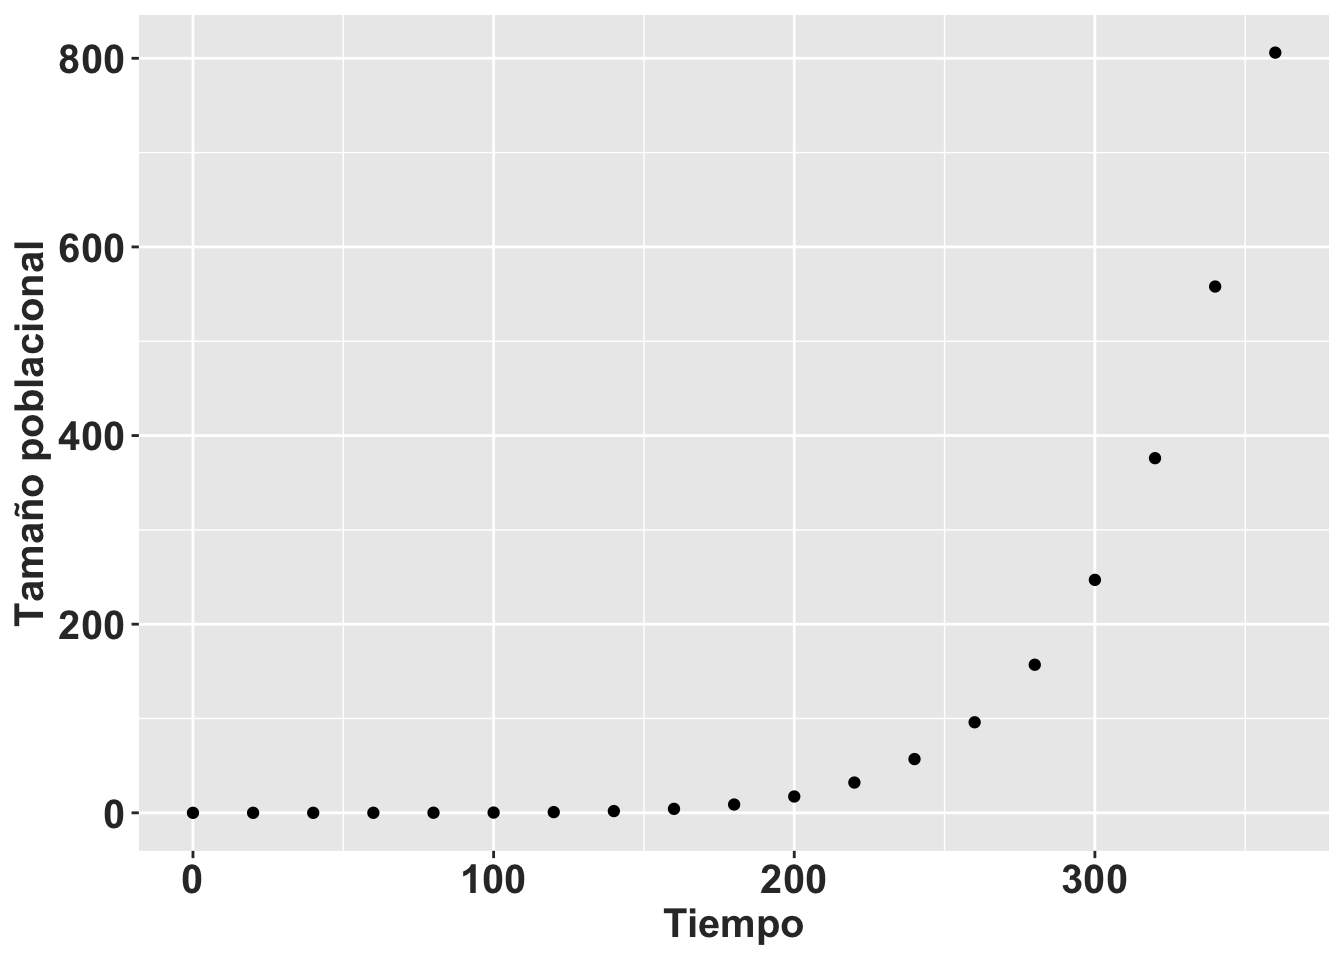
\includegraphics{Dinamica_poblacional_files/figure-latex/Pop-fig-1.pdf}
\caption{\label{fig:Pop-fig}Cambio poblacional en tiempo}
\end{figure}

\hypertarget{el-analisis-de-dinuxe1mica-poblacional-y-su-uso}{%
\section{El analisis de Dinámica Poblacional y su uso}\label{el-analisis-de-dinuxe1mica-poblacional-y-su-uso}}

Determinar el tamaño poblacional en el futuro tiene muchos usos. Se puede dividir sus usos en tres grupos grandes, entender las \textbf{1)} interacciones ecológicas, \textbf{2)} manejo y conservaciones o \textbf{3)} los procesos evolutivos. Los estudios enfocado a la conservación se engloba dentro de un acercamiento de la viablidad de poblaciones. En este libro estaremos dando una introducción a cada uno de estas vertientes, pero nuestros ejemplos son una introducción al tema y no una profundización extensa de cada uno. En la table \ref{USO} vemos algunos de los usos especificos que se ha dado con la metodología de PPM.

\hypertarget{USO}{%
\subsection{Tabla: El uso potencial de la diferentes acercamiento de PPM.}\label{USO}}

NOTA IMPORTANTE: \emph{Evaluar las referencias y añadir referencias tradicionales y recientes}

\begin{longtable}[]{@{}
  >{\raggedright\arraybackslash}p{(\columnwidth - 6\tabcolsep) * \real{0.2297}}
  >{\raggedright\arraybackslash}p{(\columnwidth - 6\tabcolsep) * \real{0.2703}}
  >{\raggedright\arraybackslash}p{(\columnwidth - 6\tabcolsep) * \real{0.2297}}
  >{\raggedleft\arraybackslash}p{(\columnwidth - 6\tabcolsep) * \real{0.2703}}@{}}
\toprule\noalign{}
\begin{minipage}[b]{\linewidth}\raggedright
Categoria de Uso
\end{minipage} & \begin{minipage}[b]{\linewidth}\raggedright
Uso especifico
\end{minipage} & \begin{minipage}[b]{\linewidth}\raggedright
Referencias
\end{minipage} & \begin{minipage}[b]{\linewidth}\raggedleft
Referencias con Oquideas
\end{minipage} \\
\midrule\noalign{}
\endhead
\bottomrule\noalign{}
\endlastfoot
Manejo & Identificar las etapas or procesos demograficos claves & \citep{crouse1987stage} & ? \\
& Determinar cuantos individuos en una población es necesario para reducir la extinción & Shaffer 1981 Armbruster \& Lande 1993 & ? \\
& Determinar cuantos individuos se necesita introducir en una sitio para establecer una población viable & Bustamante 1996 & ? \\
& Determinar cuantos individuos se puede extraer si tener un impacto negativo sobre la viabilidad de una población & Nantel et al.~1996 & ? \\
& En especies invasivas determinar cuantos y cual etapas se necesita remover para controlar la población & ? & ? \\
& Determinar cuantas pobalciones se necesita para la viabilidad de una especie al nivel local o global & Lindenmayer \& Possingham 1996 & \\
Evaluación de riesgos & Evaluar el riesgo de una población & Samson 1985 & muchos \\
& Comparando el riesgo relativo de dos o más poblaciones & Allendrof et al.~1997 & ? \\
Interacciones ecologicas & Evaluar interacciones ecológicas para entender las variables importantes para la supervivencia de una población & ? & Ospina et al., 2022 \\
Procesos y patrones evolutivos & Cual de los procesos y patrones evolutivos del ciclo de vida de especies impacta su crecimiento & ? & ? \\
\end{longtable}

\hypertarget{uso-1-identificar-las-etapas-or-procesos-demogruxe1ficos-claves}{%
\subsection{USO 1: Identificar las etapas or procesos demográficos claves}\label{uso-1-identificar-las-etapas-or-procesos-demogruxe1ficos-claves}}

Identificar y conocer cuales son las etapas de vida más suceptibles a cambios abioticos y bioticos y su impacto sobre la persistencia de una población es necesario para el manejo. El ejemplo clásico en la literatura usando PPM son los trabajos sobre la dinámica poblacional de la tortuga ``boba'' o ``cabezona'' \emph{Caretta caretta} \citep{crouse1987stage}, \citep{crowder1994predicting}. Crouse y Crowder demostrarón que aun salvando TODOS los huevos de depredación, esa estrategia de manejo antropogenico iba a tener muy poco impacto en el crecimiento de la población. Lo que econtrarón es que el impacto más grande sobre el crecimiento poblacional provendría de proteger los adultos de las redes de pesca, modificando estas para que las tortugas se pueden escapar y no ahogarse en las redes. Los trabajos de Crouse y Crowder fueron pioneros en demostrar que uno podía simular diferentes escenarios basado en la historia de vida y evaluar su impacto.

Ejemplo de orquidea AQUI

\hypertarget{uso-2-determinar-cuantos-individuos-en-una-poblaciuxf3n-es-necesario-para-reducir-la-extinciuxf3n}{%
\subsection{USO 2: Determinar cuantos individuos en una población es necesario para reducir la extinción}\label{uso-2-determinar-cuantos-individuos-en-una-poblaciuxf3n-es-necesario-para-reducir-la-extinciuxf3n}}

El efecto de tamaño poblacional sobre la biología y la probabilidad de extincción es amplia \citep{shaffer1985population}, \citep{nunney1993assessing}, \citep{harris2022abundance}. ¿Cual es la probablidad de extincción de una población considerando la cantidad de individuos en cada etapa? En general lo que se observa es que menor el tamaño poblacional, N, mayor es el riesgo de extincción. Esa probabilidad de extincción puede variar si algunas etapas del ciclo de vida tiene es muy reducido o su probabilidad de sobrevivir o crecer varia. Consideramos por ejemplo en las orquídeas donde la probabilidad de que las semillas se establece, germina y crezca a a ser un juvenil es muy pequeña. Por consecuencia una nueva población de orquidea necesita considerar la cantidad de individuos que este presente pero tambien la probabilidad de tener semillas y que estas pueden crecer a ser adultos reproducible.

\hypertarget{uso-3-determinar-cuantos-individuos-se-necesita-introducir-en-una-sitio-para-establecer-una-poblaciuxf3n-viable}{%
\subsection{USO 3: Determinar cuantos individuos se necesita introducir en una sitio para establecer una población viable}\label{uso-3-determinar-cuantos-individuos-se-necesita-introducir-en-una-sitio-para-establecer-una-poblaciuxf3n-viable}}

Naturalmente, más cantidad de individuos re-introducido en un sitio mayor sera la probabilidad que la población sea viable. Pero, como todo hay un limite de tiempo y esfuerzo disponible. Por consecuencia la pregunta debería ser orientado a determinar cual es el minimo de individuos que se deberia introductir para garantizar un x porciento de suceso en el establecimiento de una nueva población.

En los ultimos años, muchas organizaciones y cientificos han comenzado a hacer re-introducción de especies en su habitat nativo y no. (ref). Algunos programa introduce especies en areas urbanas.

\begin{itemize}
\tightlist
\item
  Caladenia
\item
  Korea
\item
  one million orchids project
\item
  ????
\end{itemize}

\hypertarget{uso-4-determinar-cuantos-individuos-se-puede-extraer-sin-tener-un-impacto-negativo-sobre-la-viabilidad-de-una-poblaciuxf3n}{%
\subsection{USO 4: Determinar cuantos individuos se puede extraer sin tener un impacto negativo sobre la viabilidad de una población}\label{uso-4-determinar-cuantos-individuos-se-puede-extraer-sin-tener-un-impacto-negativo-sobre-la-viabilidad-de-una-poblaciuxf3n}}

Hay tres razones principales para la extracción de individuos de su ambiente natural.

\begin{enumerate}
\def\labelenumi{\arabic{enumi}.}
\tightlist
\item
  Obtener individuos para la conservación \emph{Ex Situ}.
\item
  Usar un grupo de individuos para su propagación.
\item
  Extraccíon para la venta sin objetivo de conservación.
\end{enumerate}

El supuesto de colectores de orquidea de su habitat naturales, tanto para la conservación de \emph{Ex situ} y el uso para la propagación es que el impacto es minimo, y no tendrá impacto a largo plazo para la supervivencia. Regresaremos sobre este punto más tarde. La historia de fanatisismo de recolección de orquideas para la venta es bien conocida ref(). Aun que uno quisiera pensar que estas extracciones son del pasado y no occuren hoy en dia, hay todavia escrupulos que extraen los plantas sin pensar al impacto que tendrá sobre la población o especie.

Pero la pregunta se tiene que hacer. Cuantos individuos y de que etapas se puede extraer de la población sin tener impacto en el crecimoento poblacional?

\hypertarget{uso-5-en-especies-invasivas-determinar-cuantos-y-cual-etapas-se-necesita-remover-para-controlar-la-poblaciuxf3n.}{%
\subsection{USO 5: En especies invasivas determinar cuantos y cual etapas se necesita remover para controlar la población.}\label{uso-5-en-especies-invasivas-determinar-cuantos-y-cual-etapas-se-necesita-remover-para-controlar-la-poblaciuxf3n.}}

\hypertarget{uso-6-evaluar-el-riesgo-de-una-poblaciuxf3n}{%
\subsection{USO 6: Evaluar el riesgo de una población}\label{uso-6-evaluar-el-riesgo-de-una-poblaciuxf3n}}

\hypertarget{uso-7-determinar-cuantas-poblaciones-se-necesita-para-la-viabilidad-de-una-especie-al-nivel-local-o-global}{%
\subsection{USO 7: Determinar cuantas poblaciones se necesita para la viabilidad de una especie al nivel local o global}\label{uso-7-determinar-cuantas-poblaciones-se-necesita-para-la-viabilidad-de-una-especie-al-nivel-local-o-global}}

Dinamica de metapoblaciones.

\hypertarget{uso-8-comparando-el-riesgo-relativo-de-dos-o-muxe1s-poblaciones}{%
\subsection{USO 8: Comparando el riesgo relativo de dos o más poblaciones}\label{uso-8-comparando-el-riesgo-relativo-de-dos-o-muxe1s-poblaciones}}

\hypertarget{uso-9-evaluar-interacciones-ecoluxf3gicas-para-entender-las-variables-importantes-para-la-supervivencia-de-una-poblaciuxf3n}{%
\subsection{USO 9: Evaluar interacciones ecológicas para entender las variables importantes para la supervivencia de una población}\label{uso-9-evaluar-interacciones-ecoluxf3gicas-para-entender-las-variables-importantes-para-la-supervivencia-de-una-poblaciuxf3n}}

\hypertarget{uso-10-cual-de-los-procesos-y-patrones-evolutivos-del-ciclo-de-vida-de-especies-impacta-su-crecimiento}{%
\subsection{USO 10: Cual de los procesos y patrones evolutivos del ciclo de vida de especies impacta su crecimiento}\label{uso-10-cual-de-los-procesos-y-patrones-evolutivos-del-ciclo-de-vida-de-especies-impacta-su-crecimiento}}

\hypertarget{historia-de-dinamica-poblacional-en-orquideas.}{%
\section{Historia de dinamica poblacional en orquideas.}\label{historia-de-dinamica-poblacional-en-orquideas.}}

\hypertarget{referencias}{%
\section{Referencias}\label{referencias}}

\hypertarget{quuxe9-es-un-diagrama-de-ciclo-de-vida}{%
\chapter{Qué es un diagrama de Ciclo de Vida}\label{quuxe9-es-un-diagrama-de-ciclo-de-vida}}

Por: Nhora Ospina

\hypertarget{ejemplos-de-ciclos-de-vida}{%
\section{Ejemplos de ciclos de Vida}\label{ejemplos-de-ciclos-de-vida}}

Escribo algo

\hypertarget{ejemplos-de-un-ciclo-de-vida-sencillo}{%
\section{Ejemplos de un ciclo de vida sencillo}\label{ejemplos-de-un-ciclo-de-vida-sencillo}}

Tengo mucho texto que ampliar

\hypertarget{ejemplo-de-un-ciclo-de-vida-con-3-estadios}{%
\section{Ejemplo de un ciclo de vida con 3 estadios}\label{ejemplo-de-un-ciclo-de-vida-con-3-estadios}}

\begin{Shaded}
\begin{Highlighting}[]
\FunctionTok{library}\NormalTok{(Rage)}
\end{Highlighting}
\end{Shaded}

Los colores no son necesarios

\begin{Shaded}
\begin{Highlighting}[]
\CommentTok{\# hidden code to produce figures}
\FunctionTok{library}\NormalTok{(DiagrammeR)}
\NormalTok{matA }\OtherTok{\textless{}{-}} \FunctionTok{rbind}\NormalTok{(}
  \FunctionTok{c}\NormalTok{(}\FloatTok{0.0}\NormalTok{, }\FloatTok{0.0}\NormalTok{, }\FloatTok{3.2}\NormalTok{),}
  \FunctionTok{c}\NormalTok{(}\FloatTok{0.5}\NormalTok{, }\FloatTok{0.3}\NormalTok{, }\FloatTok{0.8}\NormalTok{),}
  \FunctionTok{c}\NormalTok{(}\FloatTok{0.0}\NormalTok{, }\FloatTok{0.4}\NormalTok{, }\FloatTok{0.9}\NormalTok{)}
\NormalTok{)}
\NormalTok{stages }\OtherTok{\textless{}{-}} \FunctionTok{c}\NormalTok{(}\StringTok{"seedling"}\NormalTok{, }\StringTok{"rosette"}\NormalTok{, }\StringTok{"flowering"}\NormalTok{)}
\NormalTok{title }\OtherTok{\textless{}{-}} \ConstantTok{NULL}
\NormalTok{graph }\OtherTok{\textless{}{-}} \FunctionTok{expand.grid}\NormalTok{(}\AttributeTok{to =}\NormalTok{ stages, }\AttributeTok{from =}\NormalTok{ stages)}
\NormalTok{graph}\SpecialCharTok{$}\NormalTok{trans }\OtherTok{\textless{}{-}} \FunctionTok{round}\NormalTok{(}\FunctionTok{c}\NormalTok{(matA), }\DecValTok{3}\NormalTok{)}
\NormalTok{graph }\OtherTok{\textless{}{-}}\NormalTok{ graph[graph}\SpecialCharTok{$}\NormalTok{trans }\SpecialCharTok{\textgreater{}} \DecValTok{0}\NormalTok{, ]}
\NormalTok{nodes }\OtherTok{\textless{}{-}} \FunctionTok{paste}\NormalTok{(}\FunctionTok{paste0}\NormalTok{(}\StringTok{"\textquotesingle{}"}\NormalTok{, stages, }\StringTok{"\textquotesingle{}"}\NormalTok{), }\AttributeTok{collapse =} \StringTok{"; "}\NormalTok{)}
\NormalTok{graph}\SpecialCharTok{$}\NormalTok{min\_len }\OtherTok{\textless{}{-}}\NormalTok{ (}\FunctionTok{as.numeric}\NormalTok{(graph}\SpecialCharTok{$}\NormalTok{to) }\SpecialCharTok{{-}} \FunctionTok{as.numeric}\NormalTok{(graph}\SpecialCharTok{$}\NormalTok{from)) }\SpecialCharTok{*} \DecValTok{3}
\NormalTok{graph}\SpecialCharTok{$}\NormalTok{col }\OtherTok{\textless{}{-}} \FunctionTok{c}\NormalTok{(}
  \StringTok{"PaleGreen4"}\NormalTok{, }\StringTok{"PaleGreen4"}\NormalTok{, }\StringTok{"PaleGreen4"}\NormalTok{, }\StringTok{"Goldenrod1"}\NormalTok{,}
  \StringTok{"MediumOrchid4"}\NormalTok{, }\StringTok{"PaleGreen4"}
\NormalTok{)}
\NormalTok{edges }\OtherTok{\textless{}{-}} \FunctionTok{paste0}\NormalTok{(}\StringTok{"\textquotesingle{}"}\NormalTok{, graph}\SpecialCharTok{$}\NormalTok{from, }\StringTok{"\textquotesingle{}"}\NormalTok{, }\StringTok{" {-}\textgreater{} "}\NormalTok{, }\StringTok{"\textquotesingle{}"}\NormalTok{, graph}\SpecialCharTok{$}\NormalTok{to, }\StringTok{"\textquotesingle{}"}\NormalTok{,}
  \StringTok{"[minlen="}\NormalTok{, graph}\SpecialCharTok{$}\NormalTok{min\_len,}
  \StringTok{",fontsize="}\NormalTok{, }\DecValTok{10}\NormalTok{,}
  \StringTok{",color="}\NormalTok{, graph}\SpecialCharTok{$}\NormalTok{col,}
  \StringTok{",xlabel="}\NormalTok{, }\FunctionTok{paste}\NormalTok{(}\StringTok{"}\SpecialCharTok{\textbackslash{}"}\StringTok{"}\NormalTok{, graph}\SpecialCharTok{$}\NormalTok{trans),}
  \StringTok{"}\SpecialCharTok{\textbackslash{}"}\StringTok{]}\SpecialCharTok{\textbackslash{}n}\StringTok{"}\NormalTok{,}
  \AttributeTok{collapse =} \StringTok{""}
\NormalTok{)}
\FunctionTok{grViz}\NormalTok{(}
  \FunctionTok{paste}\NormalTok{(}
    \StringTok{"}
\StringTok{digraph \{}
\StringTok{  \{}
\StringTok{    graph[overlap=false];}
\StringTok{    rank=same;}
\StringTok{    node [shape="}\NormalTok{, }\StringTok{"egg"}\NormalTok{, }\StringTok{", fontsize="}\NormalTok{, }\DecValTok{12}\NormalTok{, }\StringTok{"];"}\NormalTok{,}
\NormalTok{    nodes, }\StringTok{"}
\StringTok{  \}"}\NormalTok{,}
    \StringTok{"ordering=out}
\StringTok{  x [style=invis]}
\StringTok{  x {-}\textgreater{} \{"}\NormalTok{, nodes, }\StringTok{"\} [style=invis]"}\NormalTok{, edges,}
    \StringTok{"labelloc=}\SpecialCharTok{\textbackslash{}"}\StringTok{t}\SpecialCharTok{\textbackslash{}"}\StringTok{;}
\StringTok{  label=}\SpecialCharTok{\textbackslash{}"}\StringTok{"}\NormalTok{, title, }\StringTok{"}\SpecialCharTok{\textbackslash{}"}
\StringTok{\}"}
\NormalTok{  )}
\NormalTok{)}
\end{Highlighting}
\end{Shaded}

\begin{verbatim}
## PhantomJS not found. You can install it with webshot::install_phantomjs(). If it is installed, please make sure the phantomjs executable can be found via the PATH variable.
\end{verbatim}

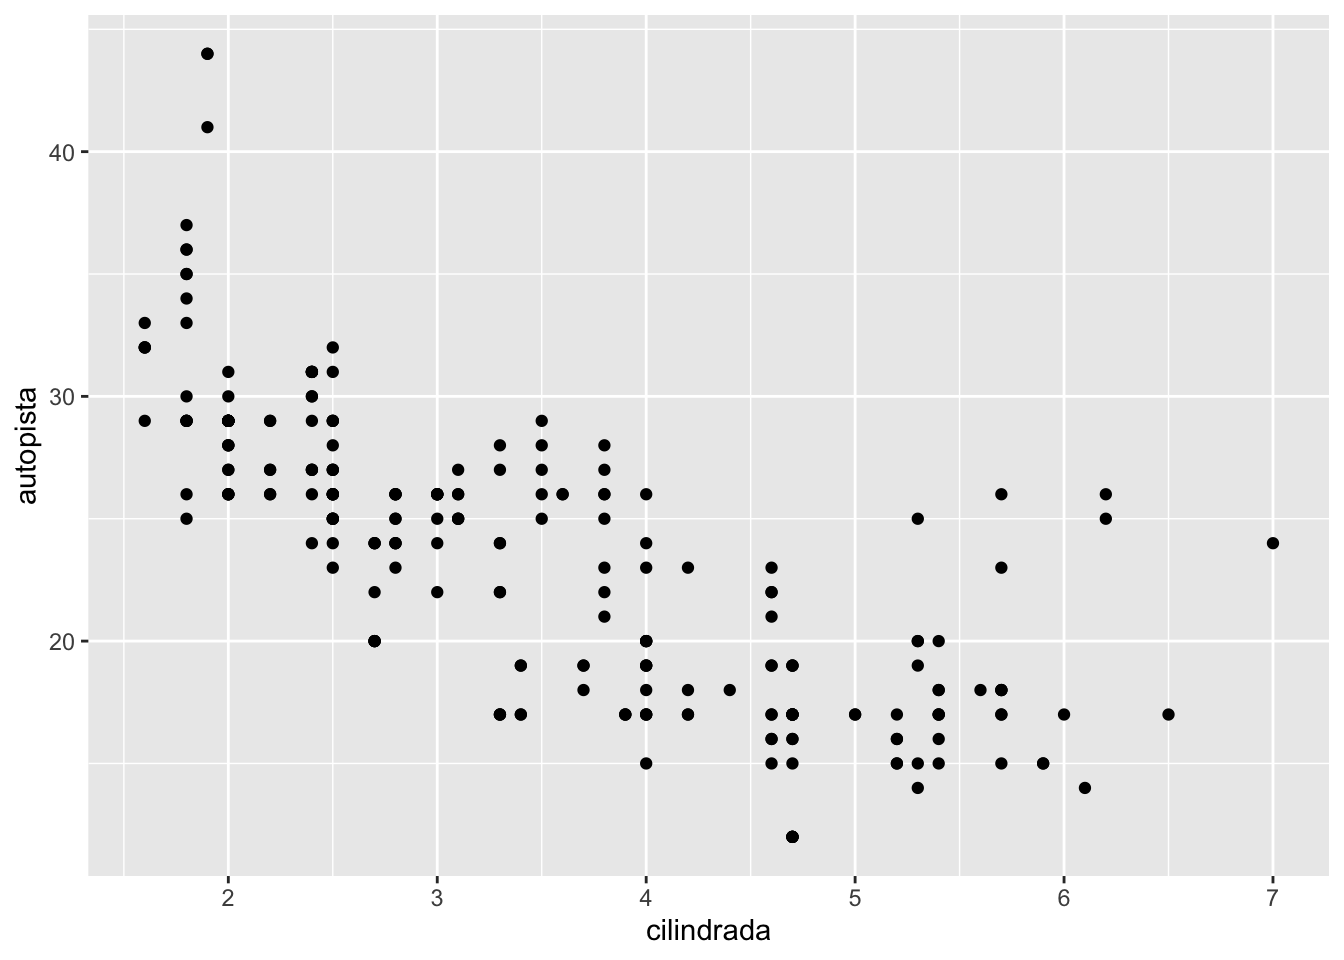
\includegraphics{Dinamica_poblacional_files/figure-latex/unnamed-chunk-3-1.pdf}

\hypertarget{ejemplo-de-un-cicle-de-vida-con-estadio-de-latencia}{%
\section{Ejemplo de un cicle de vida con estadio de latencia}\label{ejemplo-de-un-cicle-de-vida-con-estadio-de-latencia}}

\begin{Shaded}
\begin{Highlighting}[]
\FunctionTok{plot\_life\_cycle}\NormalTok{(matA, }\AttributeTok{stages=}\NormalTok{stages, }\AttributeTok{fontsize =} \DecValTok{0}\NormalTok{)}
\end{Highlighting}
\end{Shaded}

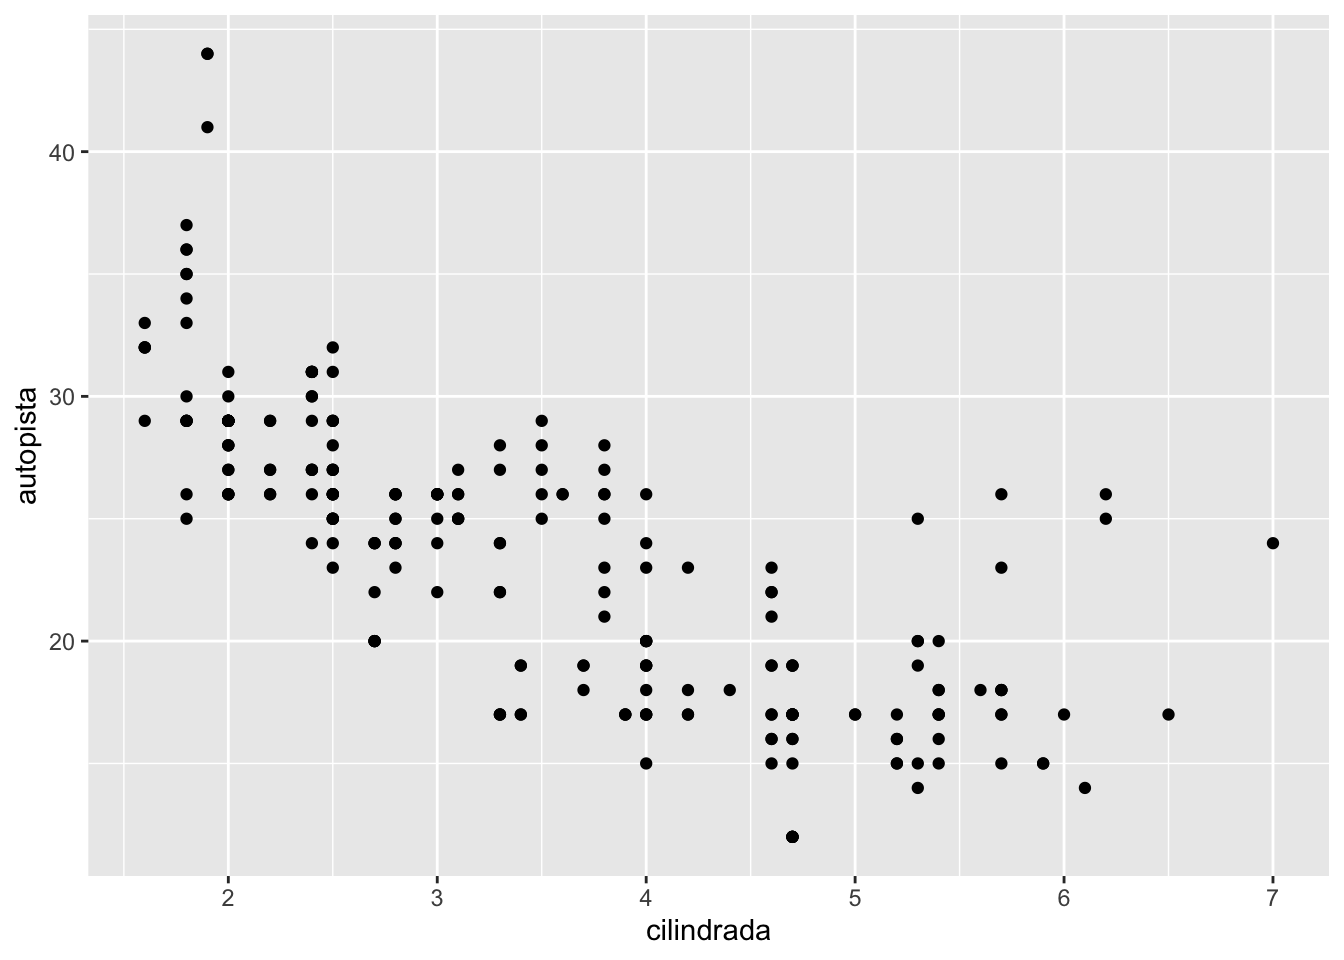
\includegraphics{Dinamica_poblacional_files/figure-latex/unnamed-chunk-4-1.pdf}

\hypertarget{code-for-color-coding-figure}{%
\section{Code for color coding figure}\label{code-for-color-coding-figure}}

\url{http://rich-iannone.github.io/DiagrammeR/}

\hypertarget{ejemplo-de-un-cicle-de-vida-con-estadio-de-post-reproducciuxf3n}{%
\section{Ejemplo de un cicle de vida con estadio de post reproducción}\label{ejemplo-de-un-cicle-de-vida-con-estadio-de-post-reproducciuxf3n}}

\hypertarget{ejemplo-de-un-cicle-de-vida-incompleto-y-biologicamente-erroneos}{%
\section{Ejemplo de un cicle de vida incompleto (y biologicamente erroneos)}\label{ejemplo-de-un-cicle-de-vida-incompleto-y-biologicamente-erroneos}}

\hypertarget{referencias-1}{%
\section{Referencias}\label{referencias-1}}

\hypertarget{como-recopilar-datos-en-el-campo}{%
\chapter{Como recopilar datos en el campo}\label{como-recopilar-datos-en-el-campo}}

Por: Raymond L. Tremblay

\hypertarget{identificar-la-especie-de-estudio}{%
\section{Identificar la especie de estudio}\label{identificar-la-especie-de-estudio}}

Para cualquier studio usando el acercamiento de dinamica poblacional es necesario conocer lo básico de la especie de interes y las etapas/edades que corresponde al ciclo de vida de esa misma. Poder reconocer las semillas, plántulas, juveniles y adultos. Algunos retos en en el estudio de las orquideas es el siguimiento de las semillas y plántulas en el campo. La dispersión de las semillas en espacio ha sido estudiado muy poco ( Sabat. et al.~) debido a sus tamaños tan pequeños y dificultad de seguir en el espacio. Los métodos de seguir las semillas en su ambiente natural incluye tipicamente ponerlos en una malla y ponerlos en el suelo o la corteza y recogerlos más tarde para ver si estas germinaron (ref).

Identificar plántulas en orquídeas terrestres tiende también a ser muy complidado, ya que están escondidas entre vegetación o cubierta de tierra. La orquideas epitifas, en ciertas especies se puede identificar las plántulas (si no están cubierta de musgo o otra vegetación), pero distinguir entre plántuls de diferentes especies puede ser imposible. Por ejemplo distinguir las plántulas de diferentes especies de \emph{Lepanthes} en el mismo forofito no es posible (Tremblay comunicación personal). El método de identificar a que especie pertenece fue de seguir estos individuos a las otras etapas (junenil o adulto). Por ejemplo la forma de crecimiento del tallo es diferente entre \emph{Lepanthes eltoroensis} (prostate) versus \emph{Lepanthes woodburyana} (erect). Por consecuencia idividuos que no sobreviven a la próxima etapa no se sabe a que especie pertenece.

\hypertarget{marcar-los-individuos-en-el-campo}{%
\section{Marcar los individuos en el campo}\label{marcar-los-individuos-en-el-campo}}

Los calidad de los métodos de marcar plantas en el campo para evaluación posterior es primordial para los análisis de dinámica poblacional. Como se marca y cual es la calidad del marcador para detectar y re-evaluar los individuos en años subsiguiente afecta la calidad de los datos. Si los marcadores individuales se pierden y no se reconoce ese problema, los individuos perdidos por marca no permanente se podría categorizar como muerto, y ese individuo no marcado (por haber perdido su identificación) pudiese ser interpretado como un nuevo individuo (reclutamiento). Eso resulta en aumento en mortandad y reclutamiento, sesgando los resultados. Naturalmente, ese sesgo depende de la frecuencia proporcional al tamaño de muestra, menor el tamaño de muestra mayor el sesgo.

El marcados tiene que ser permanente (plástico, metal, etc.) y fácil de encontrar en adición de ser informativo y único para cada planta y reducir las incertidumbres. La dificultad muchas veces proviene de individuos donde los datos son recopilados con numeración similares. Esos problemas muchas veces encuentra años después cuando se quiere re-evaluar los datos y no hay manera aclarar las dudas.

\hypertarget{muxe9todos-de-marca-y-recaptura}{%
\subsection{Métodos de marca y recaptura}\label{muxe9todos-de-marca-y-recaptura}}

\hypertarget{indentificaciones-de-individuos}{%
\subsubsection{Indentificaciones de individuos}\label{indentificaciones-de-individuos}}

Cada planta tiene que tener si propia identificación y que no haya confusión con otros individuos de esa misma población o de otra población.

\hypertarget{una-poblaciuxf3n}{%
\paragraph{Una población}\label{una-poblaciuxf3n}}

Por ejemplo si el estudio comenzó en 2023 y solamente hay una población. Los individuos podrían tener una codificación siguiente 23001, 23002, 23003, \ldots{} 23152 para los 152 individuos encontrado y marcado ese año. El siguiente año se muestra esos individuos y nuevos individuos encontrado comenzarían con 24153. De esta forma ya se conoce cuando fue el primer año de muestreo del individuo y esos nuevos individuos no se confunde con los del año anterior. Cada año comenzaría con identificación del año, y la numeración de los individuos no se repiten en la misma población. Entonces hay redundandia en la codificación ayudando a reducir los errores de codificaciones.

\hypertarget{multiples-poblaciones}{%
\subparagraph{Multiples poblaciones}\label{multiples-poblaciones}}

Siguiendo con el mismo concepto pero múltiples poblaciones, la numeración de la población pudiese utilizar una codificación alfa numérica, donde la letra del alfabeto representa la población y la número los individuos. Siguiera así A23001, A23002,\ldots, 23xxx para la primera población y B23001, B23002,\ldots, B23xxx para las segunda población.

\hypertarget{relocalizaciuxf3n-de-individuos}{%
\subsection{Relocalización de individuos}\label{relocalizaciuxf3n-de-individuos}}

Para relocalizar los individuos se puede utilizar marcador permanentes o geo-referencias individuales para cada planta.

Métodos de relocalizar los individuos en el campo puede ser complicado.

\begin{itemize}
\tightlist
\item
  uno de los métodos es amarar al individuo la identificación individual de forma que se fácil de encontrar y que no se pierde. Por ejemplo uno puede amarar el ``tag'' con hilo de pezcar grueso o ``twist tags'' alrededor de unos pseudobulbos o cerca de la planta. El la foto que sigue vemos una planta \emph{Cypripedium acaule} en la región de North Bay, Ontario, Canada marcado con un tag metálico cerca de la planta
\end{itemize}

\begin{figure}
\centering
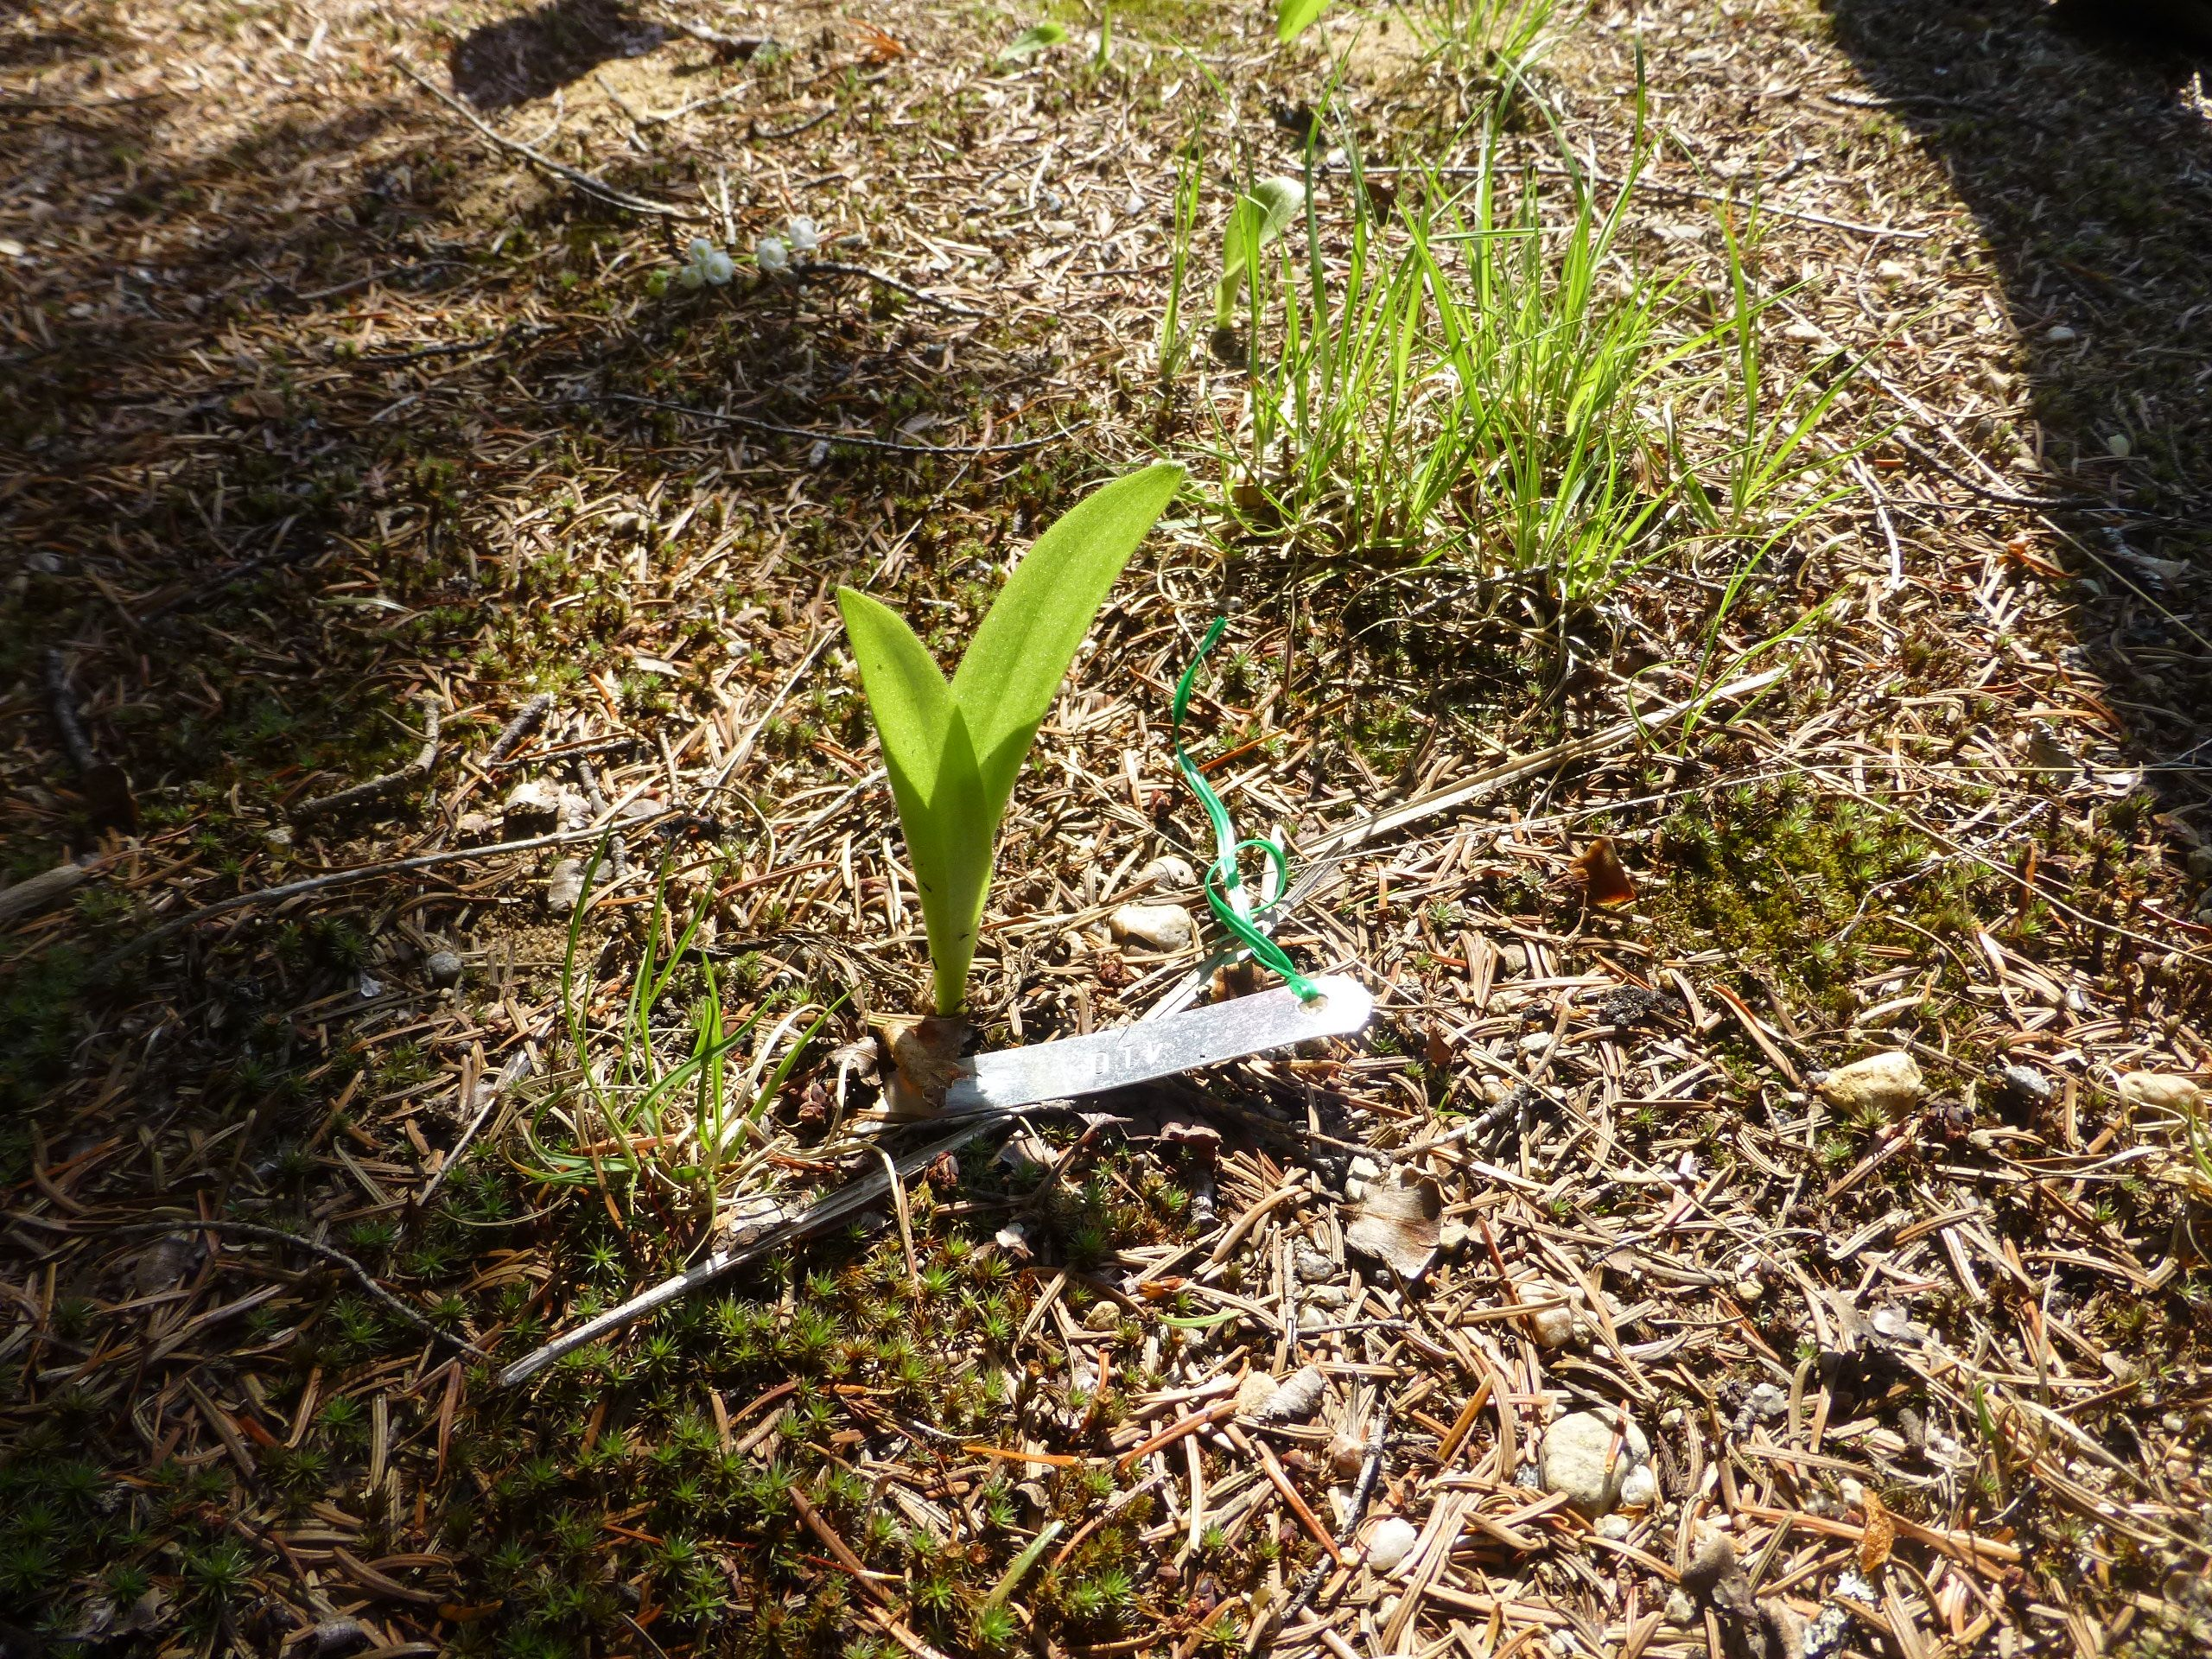
\includegraphics[width=0.5\textwidth,height=\textheight]{Figures/Cypripedium_acaule.jpg}
\caption{Cypripedium acaule marcado; Foto: Tremblay}
\end{figure}

\textbf{Necesitamos unos ejemplos}

\begin{itemize}
\tightlist
\item
  otro metodo es grapar el ``tag'' al lado de los individuos. Este es un método que es adecuado para plantas pequeñas. NO se debería poner el tag agarrado a la planta, ya que el peso del tag, podría causar daño a la planta, en adición que este caso las hojas no son persistente, por consecuencia al caer una hoja podría perder el ``tag''. En esa foto se uso un pequeño clavo para poner el ``tag'', pero también usando una grapadora puede ser más eficiente y menos dañino al árbol. En la foto siguiente se ve un tag de plastico amarado con un clavo al lado de de una planta de Lepanthes eltoroensis en Puerto Rico. Posteriormente se cambio el calvo por una grapadora normal. Ese metodofuncionó muy bien.
\end{itemize}

\begin{figure}
\centering
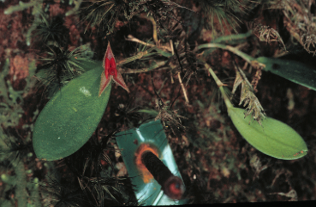
\includegraphics[width=0.5\textwidth,height=\textheight]{Figures/Lep_eltoroensis.png}
\caption{Lepanthes eltoroensis marcado; Foto: Tremblay}
\end{figure}

Si el sitio esta bien protegido y no hay riesgos de atraer atención a las plantas se puede usar pequeñas banderas para facilitar la recaptura de las plantas.

NOTA importante: los ``tags'' no deberían ser facil de ver en el habitat ya que podría atraer atención al estudio y hay mucha gente que se llevan plantas del campo, incluyendo plantas que son partes de estudios.

\begin{figure}
\centering
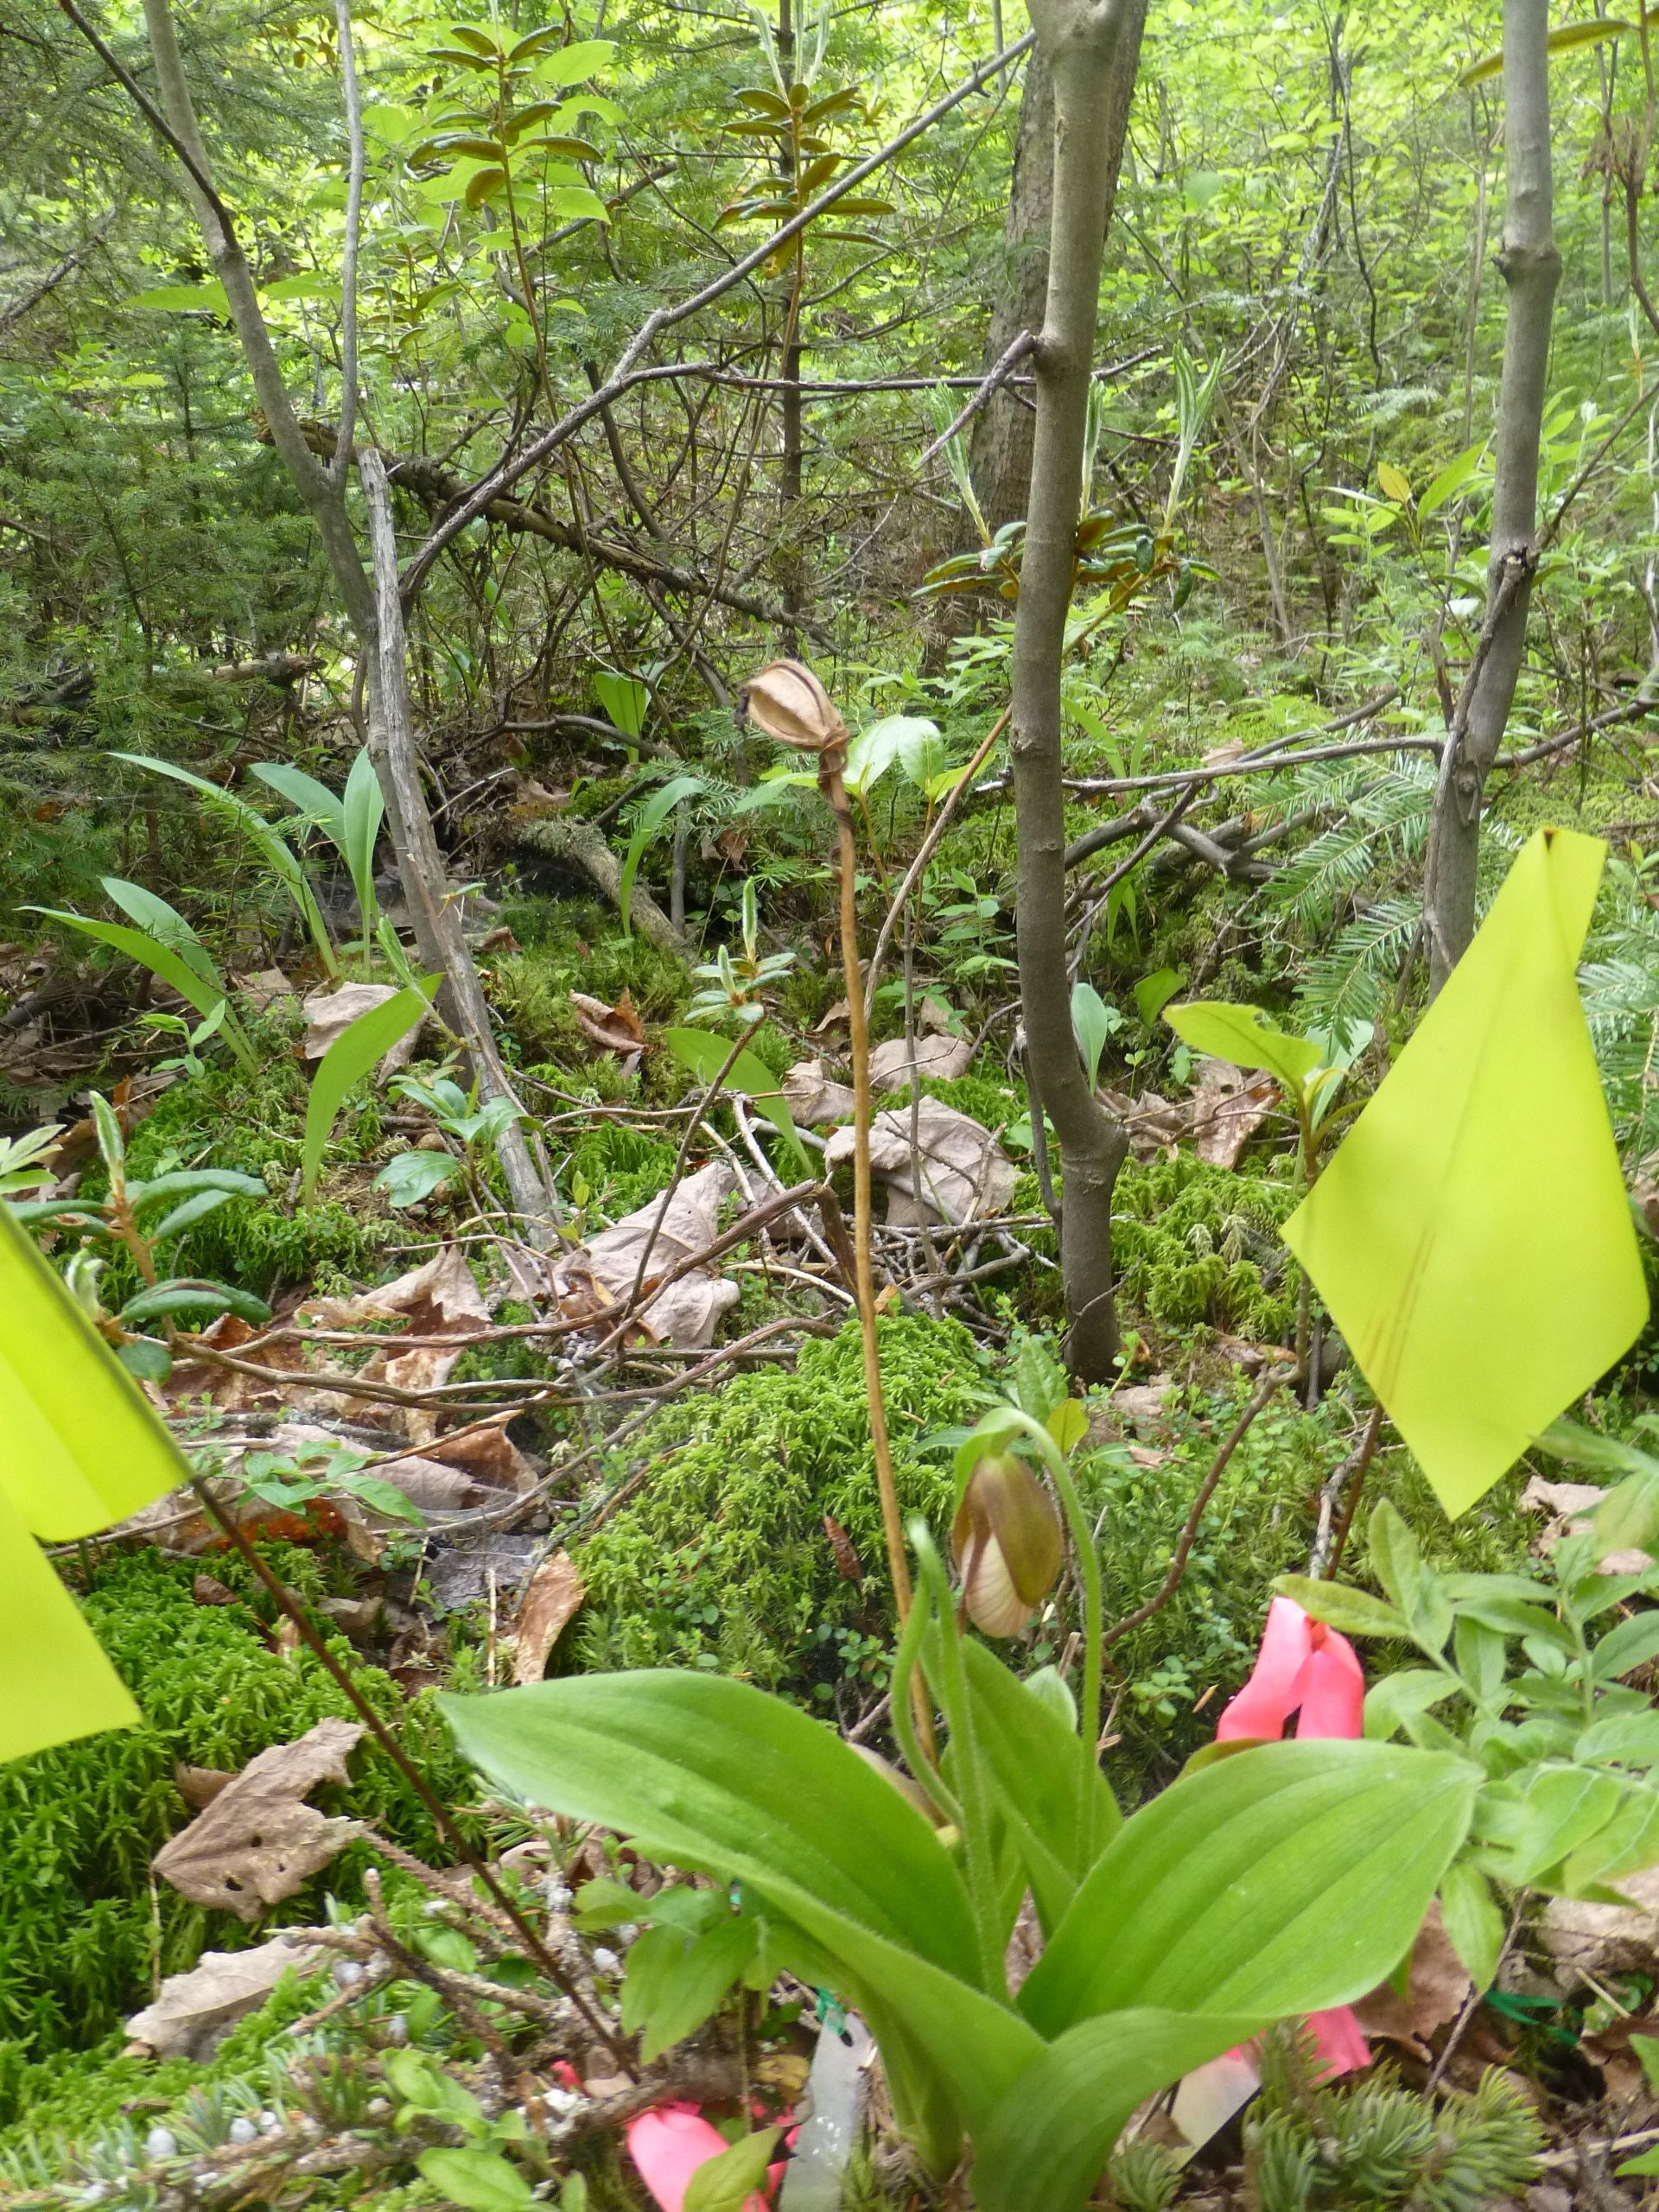
\includegraphics[width=0.5\textwidth,height=\textheight]{Figures/Cyp_acaule_flag.jpg}
\caption{Cypripedium acaule identificado con bandera numerada; Foto: Tremblay}
\end{figure}

\hypertarget{variables-a-recoger-en-el-campo}{%
\section{Variables a recoger en el campo}\label{variables-a-recoger-en-el-campo}}

La base de los estudios de dinamica poblacional es evaluar las transiciones entre las etapas de vida incluyendo mortantad y su reprodución. La información que se recoge del campo tiene que ser facil de recoger y consistente y sin error. Si seguimos ejemplos de los trabajos de campo de Tremblay {[}ref{]} con \emph{Lepanthes}, las etapas incluidas son plantulas, juveniles, adultos no reproductivos y adultos reproductivos. Cada una de estas estapas estan definida especificamente para ese genero.

\begin{itemize}
\tightlist
\item
  \textbf{plantula}: individuo que no tiene ninguna hoja con peciolo.
\item
  \textbf{juvenil}: individuo que tiene hojas con peciolo pero no hay ninguna evidencia que fue reproductiva en el pasado (las base de las inflorescencia son persistente)
\item
  \textbf{adulto non-reproductivo}: individuos con inflorescencias secas (ninguna verde)
\item
  \textbf{adulto reproductivo}: individuo con inflorescencia verdes con o sin flores o frutos.
\end{itemize}

Dependiendo de los estudios pudiese haber más etapas, por ejemplo Tremblay {[} {]} uso dos etapas de individuos reproductivos.

Otro ejemplo es el estudio de Hernández-Apolinar con la especie xx. donde incluyo\ldots..

Determinar cuantas categoria deberia ser utilizados y cuales es muy dinamica y depende de la especies, número individuos y las preguntas de interes.

Las variables a recoger tiene que incluir el minimo las siguientes

\begin{itemize}
\tightlist
\item
  la etapa en el tiempo t
\item
  si esta vivo o muerto en el tiempo t
\item
  la cantidad de flores en el tiempo t
\item
  la cantidad de frutos en el tiempo t
\item
  la presencia y ``tagging'' de nuevos individuos en el tiempo t+1
\end{itemize}

Otras variables que pudiese recoger incluye

\begin{itemize}
\item
  el tamaño de las hojas o la hoja más grande

  \begin{itemize}
  \tightlist
  \item
    \emph{Brasavola cucculata} {[}{]}: las plantas necesitan un tamaño minimo de largo de hoja antes de florecer
  \end{itemize}
\item
  el número de pseudobulbo

  \begin{itemize}
  \tightlist
  \item
    \ldots.
  \end{itemize}
\item
  la altura de la inflorescencia

  \begin{itemize}
  \tightlist
  \item
    \emph{Caladenia valida} {[}{]}: la altura de la inflorescencia impacta la probabilidad de producir frutos
  \end{itemize}
\item
  la altura en el árbol de las epífitas

  \begin{itemize}
  \tightlist
  \item
    \emph{Brasavola cucculata} {[}{]}: la plantas muy bajo menos de 1.5m son depredadas por la cabras
  \end{itemize}
\item
  el número de ``ramet'', un indice del tamaño del genotipo en plantas con crecimiento horizontal

  \begin{itemize}
  \tightlist
  \item
    \emph{Cypripedium calceolus var. parviflorum} {[}Tremblay{]}: Los estudios evolutivos tienen que reconocer la diferencia entre un ``ramet'' y un ``genet''.
  \end{itemize}
\item
  indicadores de herbivoria sobre la planta
\item
  indicadores de la cantidad plagas sobre la planta como ``rust''
\end{itemize}

\hypertarget{referencias-2}{%
\section{Referencias}\label{referencias-2}}

\hypertarget{como-calcular-transiciones-para-la-matriz-de-lefkovitch}{%
\chapter{Como calcular transiciones para la matriz de Lefkovitch}\label{como-calcular-transiciones-para-la-matriz-de-lefkovitch}}

\hypertarget{por-ernesto-mujica-y-elaine-gonzalez}{%
\section{Por: Ernesto Mujica y Elaine Gonzalez}\label{por-ernesto-mujica-y-elaine-gonzalez}}

\hypertarget{muxe9todos-tradicional-de-calcular-las-transiciones}{%
\section{Métodos tradicional de calcular las transiciones}\label{muxe9todos-tradicional-de-calcular-las-transiciones}}

\hypertarget{problema-con-el-uso-tradicional}{%
\section{Problema con el uso tradicional}\label{problema-con-el-uso-tradicional}}

\hypertarget{referencias-3}{%
\section{Referencias}\label{referencias-3}}

\hypertarget{como-calcular-fecundidad}{%
\chapter{Como calcular fecundidad}\label{como-calcular-fecundidad}}

\hypertarget{por-demetria-equipo-ecosur}{%
\section{Por: Demetria: equipo ECOSUR}\label{por-demetria-equipo-ecosur}}

\hypertarget{muxe9todos-tradicional-de-calcular-las-transiciones-1}{%
\section{Métodos tradicional de calcular las transiciones}\label{muxe9todos-tradicional-de-calcular-las-transiciones-1}}

\hypertarget{problema-con-el-uso-tradicional-1}{%
\section{Problema con el uso tradicional}\label{problema-con-el-uso-tradicional-1}}

\hypertarget{referencias-4}{%
\section{Referencias}\label{referencias-4}}

\hypertarget{matrices-de-transicion-fecundidad-y-clonal}{%
\chapter{Matrices de transicion, fecundidad y clonal}\label{matrices-de-transicion-fecundidad-y-clonal}}

\hypertarget{por}{%
\section{Por:??}\label{por}}

\hypertarget{muxe9todos-tradicional-de-calcular-las-transiciones-2}{%
\section{Métodos tradicional de calcular las transiciones}\label{muxe9todos-tradicional-de-calcular-las-transiciones-2}}

\hypertarget{problema-con-el-uso-tradicional-2}{%
\section{Problema con el uso tradicional}\label{problema-con-el-uso-tradicional-2}}

\hypertarget{referencias-5}{%
\section{Referencias}\label{referencias-5}}

\hypertarget{muxe9todo-bayesiano-de-calcular-las-transciones}{%
\chapter{Método bayesiano de calcular las transciones}\label{muxe9todo-bayesiano-de-calcular-las-transciones}}

Por: RLT

El objetivo de este capítulo es demostrar algunos de los retos cuando uno trabaja con especies raras o con poca información para estimar los parametros de la matrices y como se puede resolver y estimar parametros más realista.

Considera este primer ejemplo donde se estima que la especie de interes tenga tres etapas en su ciclo de vida (semillas, plantulas y adultos) y que solamente la etapa más grande (de adultez) puede producir semillas.

Cuando se comienza un analisis de dinamica poblacional el primer paso es evaluar y tratar de ver cual son las etapas del ciclo de vida que pudiesen ser representativo de la dinamica principal de la especie.

En esta primera figura vemos lo que se considerá que ocurre en esa especie hipotetica.

\begin{Shaded}
\begin{Highlighting}[]
\FunctionTok{library}\NormalTok{(Rage)}
\end{Highlighting}
\end{Shaded}

Ahora ud recoge los datos del campo y evalua las transiciones y fecundidad y tiene información siguiente.

\begin{enumerate}
\def\labelenumi{\arabic{enumi}.}
\tightlist
\item
  Todas las semilla germinan y crece a la etapa de plantula.\\
\end{enumerate}

\begin{itemize}
\tightlist
\item
  Es realista que todas las semillas germinan?
\item
  Por que no se encontró semillas que NO germinan?
\end{itemize}

\begin{enumerate}
\def\labelenumi{\arabic{enumi}.}
\setcounter{enumi}{1}
\tightlist
\item
  Todos las plantulas mueren

  \begin{itemize}
  \tightlist
  \item
    Es realista que todas las plantulas se muere?
  \end{itemize}
\end{enumerate}

Aqui se ve dos de los problemas que resulta en PPM que no son realista, uno que no hay ninguna mortantad o que todo se muere. El otro componente es el efecto del tamaño de muestra, considerá que su especie de interes Ud tuvo acceso solamente a 4 plantas adultas (un especies rara), y 4 de los 4 sobrevieron, por consecuencia 100\% de supervivencia. Si los individuos llegan a esta etapa son inmortales!!!? Claramente es un resultado del tamaño de muestra y no del ciclo de vida de la especie.

El paquete raretrans ayuda en resolver estos asuntos illogicos y crear matrices que son más entre realistas al ciclo de vida de su especie.

\begin{Shaded}
\begin{Highlighting}[]
\CommentTok{\# hidden code to produce figures}
\FunctionTok{library}\NormalTok{(DiagrammeR)}


\NormalTok{matA }\OtherTok{\textless{}{-}} \FunctionTok{rbind}\NormalTok{(}
  \FunctionTok{c}\NormalTok{(}\FloatTok{0.0}\NormalTok{, }\FloatTok{0.0}\NormalTok{, }\FloatTok{0.0}\NormalTok{),}
  \FunctionTok{c}\NormalTok{(}\FloatTok{1.0}\NormalTok{, }\FloatTok{0.0}\NormalTok{, }\FloatTok{0.0}\NormalTok{),}
  \FunctionTok{c}\NormalTok{(}\FloatTok{0.0}\NormalTok{, }\FloatTok{0.0}\NormalTok{, }\FloatTok{0.9}\NormalTok{)}
\NormalTok{)}
\NormalTok{stages }\OtherTok{\textless{}{-}} \FunctionTok{c}\NormalTok{(}\StringTok{"semillas"}\NormalTok{, }\StringTok{"plantulas"}\NormalTok{, }\StringTok{"adultos"}\NormalTok{)}
\NormalTok{title }\OtherTok{\textless{}{-}} \ConstantTok{NULL}
\end{Highlighting}
\end{Shaded}

\begin{Shaded}
\begin{Highlighting}[]
\FunctionTok{plot\_life\_cycle}\NormalTok{(matA, }\AttributeTok{stages=}\NormalTok{stages)}
\end{Highlighting}
\end{Shaded}

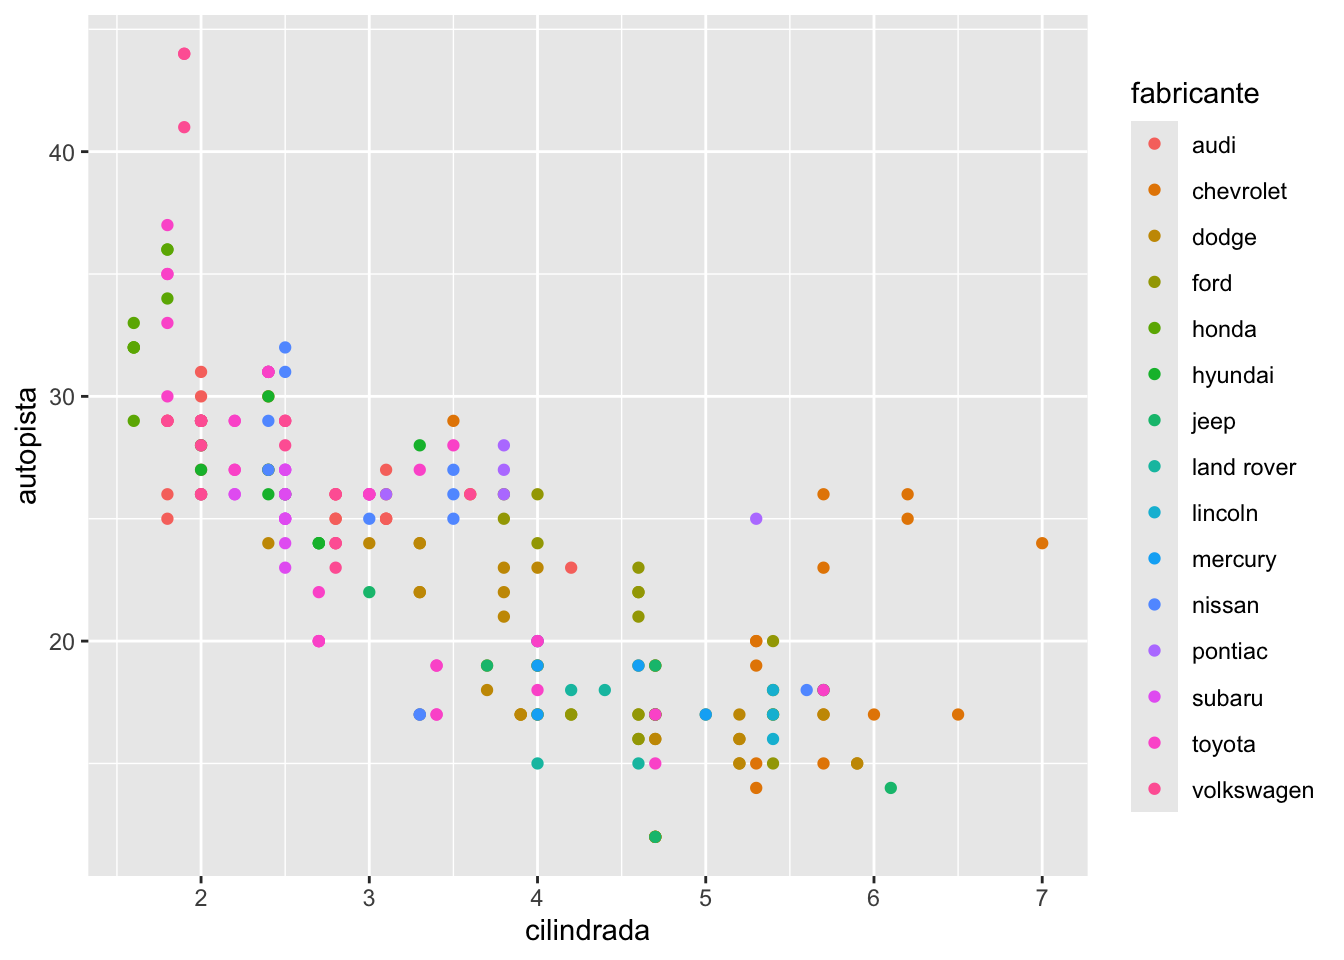
\includegraphics{Dinamica_poblacional_files/figure-latex/unnamed-chunk-7-1.pdf}

\hypertarget{el-paquete-raretrans}{%
\section{El paquete ``raretrans''}\label{el-paquete-raretrans}}

La información original del uso del paquete se encuentra aqui \url{https://doi.org/10.1016/j.ecolmodel.2021.109526}.

\textbf{Population projections from holey matrices: Using prior information to estimate rare transition events}

Abstracto

Las matrices de proyección de población son un medio común para predecir la persistencia de la población a corto y largo plazo para especies raras, amenazadas y en peligro de extinción. Los datos de tales especies pueden sufrir de tamaños de muestra pequeños y, en consecuencia, perder eventos demográficos raros que dan como resultado trayectorias de ciclo de vida incompletas o biológicamente poco realistas. Las matrices con valores faltantes (ceros; p.~ej., sin observación de semillas que se transforman en plántulas) a menudo se reparan utilizando información previa de la literatura, otras poblaciones, períodos de tiempo, otras especies, estimaciones de las mejores conjeturas o, a veces, incluso se ignoran. Para paliar este problema, proponemos usar un modelo multinomial de Dirichlet para parametrizar transiciones y un Gamma para la reproducción para parchear los valores faltantes en estas matrices perforadas. Esto integra formalmente la información previa dentro de un marco bayesiano e incluye explícitamente el peso de la información previa en las distribuciones posteriores. Mostramos utilizando dos conjuntos de datos reales que el peso asignado a la información anterior influye principalmente en la dispersión de los posteriores, la inclusión de anteriores da como resultado matrices irreducibles y ergódicas, y se pueden hacer inferencias biológicamente más realistas sobre las probabilidades de transición. Debido a que los antecedentes se establecen explícitamente, los resultados son reproducibles y se pueden volver a evaluar si hay antecedentes alternativos disponibles en el futuro.

\hypertarget{instalaciuxf3n-de-los-paquetes-1}{%
\section{Instalación de los paquetes \#1}\label{instalaciuxf3n-de-los-paquetes-1}}

\begin{Shaded}
\begin{Highlighting}[]
\ControlFlowTok{if}\NormalTok{ (}\SpecialCharTok{!}\FunctionTok{require}\NormalTok{(}\StringTok{"pacman"}\NormalTok{)) }\FunctionTok{install.packages}\NormalTok{(}\StringTok{"pacman"}\NormalTok{)}
\end{Highlighting}
\end{Shaded}

\begin{verbatim}
## Loading required package: pacman
\end{verbatim}

\begin{Shaded}
\begin{Highlighting}[]
\NormalTok{pacman}\SpecialCharTok{::}\FunctionTok{p\_load}\NormalTok{(janitor, tidyverse, devtools)}

\FunctionTok{library}\NormalTok{(tidyverse)}
\FunctionTok{library}\NormalTok{(janitor)}
\end{Highlighting}
\end{Shaded}

\hypertarget{instalaciuxf3n-de-raretrans-2}{%
\section{Instalación de raretrans \#2}\label{instalaciuxf3n-de-raretrans-2}}

\begin{Shaded}
\begin{Highlighting}[]
\CommentTok{\#library(devtools)}

\CommentTok{\#devtools::install\_github("atyre2/raretrans", build = TRUE, build\_opts = c("{-}{-}no{-}resave{-}data", "{-}{-}no{-}manual"))}

\FunctionTok{library}\NormalTok{(raretrans)}
\end{Highlighting}
\end{Shaded}

Vea el siguiente website para más información en ingles, la información que sigue es una traducción y ampliación de la información en el siuiente enlace.

\url{https://atyre2.github.io/raretrans/articles/onepopperiod.html}

\begin{Shaded}
\begin{Highlighting}[]
\FunctionTok{library}\NormalTok{(tidyverse)}
\FunctionTok{library}\NormalTok{(ggplot2)}
\FunctionTok{library}\NormalTok{(popbio) }\CommentTok{\# para la función projection.matrix()}
\FunctionTok{library}\NormalTok{(raretrans)}
\CommentTok{\# Mi tema de ggplot2 personal}
\NormalTok{rlt\_theme }\OtherTok{\textless{}{-}} \FunctionTok{theme}\NormalTok{(}\AttributeTok{axis.title.y =} \FunctionTok{element\_text}\NormalTok{(}\AttributeTok{colour=}\StringTok{"grey20"}\NormalTok{,}\AttributeTok{size=}\DecValTok{15}\NormalTok{,}\AttributeTok{face=}\StringTok{"bold"}\NormalTok{),}
        \AttributeTok{axis.text.x =} \FunctionTok{element\_text}\NormalTok{(}\AttributeTok{colour=}\StringTok{"grey20"}\NormalTok{,}\AttributeTok{size=}\DecValTok{15}\NormalTok{, }\AttributeTok{face=}\StringTok{"bold"}\NormalTok{),}
        \AttributeTok{axis.text.y =} \FunctionTok{element\_text}\NormalTok{(}\AttributeTok{colour=}\StringTok{"grey20"}\NormalTok{,}\AttributeTok{size=}\DecValTok{15}\NormalTok{,}\AttributeTok{face=}\StringTok{"bold"}\NormalTok{),  }
        \AttributeTok{axis.title.x =} \FunctionTok{element\_text}\NormalTok{(}\AttributeTok{colour=}\StringTok{"grey20"}\NormalTok{,}\AttributeTok{size=}\DecValTok{15}\NormalTok{,}\AttributeTok{face=}\StringTok{"bold"}\NormalTok{))}
\end{Highlighting}
\end{Shaded}

El objetivo de esta viñeta es demostrar el uso del paquete \texttt{raretrans}
para los calculos de los parametros en una población y periodo de
transición.

\hypertarget{parte-i-obtenciuxf3n-de-la-matriz-de-proyecciuxf3n}{%
\section{Parte I: Obtención de la matriz de proyección}\label{parte-i-obtenciuxf3n-de-la-matriz-de-proyecciuxf3n}}

\texttt{raretrans} asume que la matriz de proyección es una lista de dos
matrices, una matriz de transición y una matriz de fertilidad. Este es
el formato de salida de \texttt{popbio::projection.matrix}. Si tenemos
transiciones individuales en un marco de datos

Podemos utilizar \texttt{popbio::projection.matrix} para obtener los datos
necesarios. Hacemos una demostración con los datos de transición y
fertilidad de la orquídea epifita \emph{Lepanthes elto} \textbf{POPNUM 250} en el
\textbf{periodo 5}.

\hypertarget{paso-1-cargar-y-fusionar-los-datos-de-poblaciuxf3n-uxfanica-para-l.-elto}{%
\section{\texorpdfstring{Paso 1: Cargar y fusionar los datos de población única para \emph{L. elto}}{Paso 1: Cargar y fusionar los datos de población única para L. elto}}\label{paso-1-cargar-y-fusionar-los-datos-de-poblaciuxf3n-uxfanica-para-l.-elto}}

\begin{Shaded}
\begin{Highlighting}[]
\FunctionTok{data}\NormalTok{(}\StringTok{"L\_elto"}\NormalTok{) }\CommentTok{\# carga el conjunto de datos \textasciigrave{}L\_elto\textasciigrave{} en memoria (incluido en el paquete \textasciigrave{}raretrans\textasciigrave{})}
\FunctionTok{head}\NormalTok{(L\_elto) }
\end{Highlighting}
\end{Shaded}

\begin{verbatim}
## # A tibble: 6 x 13
##   POPNUM  year seedlings adults fertility IND_NUM stage next_stage first_year
##    <dbl> <dbl>     <dbl>  <dbl>     <dbl>   <dbl> <chr> <chr>           <dbl>
## 1    209     1         1      6         0      67 j     j                   1
## 2    209     1         1      6         0      68 a     a                   1
## 3    209     1         1      6         0      69 a     a                   1
## 4    209     1         1      6         0      70 a     a                   1
## 5    209     1         1      6         0      71 j     a                   1
## 6    209     1         1      6         0      72 a     a                   1
## # i 4 more variables: last_year <dbl>, recruited <lgl>, died <dbl>,
## #   lifespan <int>
\end{verbatim}

\hypertarget{organizaciuxf3n-de-los-datos-en-el-data.frame}{%
\section{Organización de los datos en el ``data.frame''}\label{organizaciuxf3n-de-los-datos-en-el-data.frame}}

\begin{itemize}
\tightlist
\item
  el primer paso es seleccionar los datos de una población y un
  periodo de tiempo
\item
  el segundo paso es hacer un cambio en la terminología para el estado
  más pequeño de ``plantula'' a ``seedling''\ldots{} Ese cambio es para que la
  información presentada aqui sea la misma que en el documento en
  ingles.
\end{itemize}

Cada fila de este data.frame de datos tiene columnas para la fase actual
(stage), la fase siguiente (next\_stage) y la fertilidad por individuo.
Tenga en cuenta que ``p'' significa ``plantula'' en español. El primer
conjunto de líneas de abajo cambia el nombre de la etapa del ciclo vital
de ``p'' a ``s'' después de seleccionar la población y el periodo de tiempo.

\begin{Shaded}
\begin{Highlighting}[]
\NormalTok{onepop }\OtherTok{\textless{}{-}}\NormalTok{ L\_elto }\SpecialCharTok{\%\textgreater{}\%}   
\CommentTok{\# Filtrar la población \# 250, el periodo (año=year) 5}
  \FunctionTok{filter}\NormalTok{(POPNUM }\SpecialCharTok{==} \DecValTok{250}\NormalTok{, year }\SpecialCharTok{==} \DecValTok{5}\NormalTok{) }\SpecialCharTok{\%\textgreater{}\%} 
  \CommentTok{\# redefine "p" por plantula a "s" para seedling}
  \FunctionTok{mutate}\NormalTok{(}\AttributeTok{stage =} \FunctionTok{case\_when}\NormalTok{(stage }\SpecialCharTok{==} \StringTok{"p"} \SpecialCharTok{\textasciitilde{}} \StringTok{"s"}\NormalTok{,}
                           \ConstantTok{TRUE} \SpecialCharTok{\textasciitilde{}}\NormalTok{ stage),}
         \AttributeTok{next\_stage =} \FunctionTok{case\_when}\NormalTok{(next\_stage }\SpecialCharTok{==} \StringTok{"p"}\SpecialCharTok{\textasciitilde{}} \StringTok{"s"}\NormalTok{,}
                                \ConstantTok{TRUE} \SpecialCharTok{\textasciitilde{}}\NormalTok{ next\_stage))}
\CommentTok{\# popbio::projection.matrix no funciona con tibbles, por consecuencia se convierte en data.frame}

\FunctionTok{head}\NormalTok{(onepop)}
\end{Highlighting}
\end{Shaded}

\begin{verbatim}
## # A tibble: 6 x 13
##   POPNUM  year seedlings adults fertility IND_NUM stage next_stage first_year
##    <dbl> <dbl>     <dbl>  <dbl>     <dbl>   <dbl> <chr> <chr>           <dbl>
## 1    250     5         8     34     0         167 j     a                   1
## 2    250     5         8     34     0         168 j     a                   1
## 3    250     5         8     34     0         169 j     a                   1
## 4    250     5         8     34     0.118     170 a     a                   1
## 5    250     5         8     34     0         172 j     j                   1
## 6    250     5         8     34     0         173 j     a                   1
## # i 4 more variables: last_year <dbl>, recruited <lgl>, died <dbl>,
## #   lifespan <int>
\end{verbatim}

\begin{Shaded}
\begin{Highlighting}[]
\CommentTok{\# Crear TF = TRUE, añadir para formatear corectamente.}
\NormalTok{TF }\OtherTok{\textless{}{-}}\NormalTok{ popbio}\SpecialCharTok{::}\FunctionTok{projection.matrix}\NormalTok{(}\FunctionTok{as.data.frame}\NormalTok{(onepop), }
                        \AttributeTok{stage =}\NormalTok{ stage, }\AttributeTok{fate =}\NormalTok{ next\_stage, }
                        \AttributeTok{fertility=}\StringTok{"fertility"}\NormalTok{, }\AttributeTok{sort=}\FunctionTok{c}\NormalTok{(}\StringTok{"s"}\NormalTok{,}\StringTok{"j"}\NormalTok{,}\StringTok{"a"}\NormalTok{), }\AttributeTok{TF =} \ConstantTok{TRUE}\NormalTok{)}
\NormalTok{TF }\CommentTok{\# Este es la estructura de etapas de vida para esa población }
\end{Highlighting}
\end{Shaded}

\begin{verbatim}
## $T
##    
##              s          j          a
##   s 0.09090909 0.00000000 0.00000000
##   j 0.63636364 0.57446809 0.00000000
##   a 0.00000000 0.29787234 0.85294118
## 
## $F
##    
##             s         j         a
##   s 0.0000000 0.0000000 0.1176471
##   j 0.0000000 0.0000000 0.0000000
##   a 0.0000000 0.0000000 0.0000000
\end{verbatim}

\hypertarget{nota}{%
\section{Nota:}\label{nota}}

Nuestros estadios se codifican ahora como \textbf{s} (plántula), \textbf{j}
(juvenil) y \textbf{a} (adulto), y ahora tenemos dos matrices: \textbf{T}
(transición de estadios) y \textbf{F} (fecundidad). La tasa de crecimiento
asintótico de la población observada es \(\lambda =\)
0.93. Las transiciones raras que
faltan en nuestra primera matriz de transición, \texttt{TF\$T}, son la
transición de plántula (\emph{s}) a adulto (\emph{a}) y la transición de \emph{j} a
\emph{s}. Pero sabemos que ocurren.

\hypertarget{paso-2-obtener-el-nuxfamero-inicial-de-individuos-por-etapa}{%
\section{Paso 2: Obtener el número inicial de individuos por etapa}\label{paso-2-obtener-el-nuxfamero-inicial-de-individuos-por-etapa}}

Dado que nuestras priores se basan en recuentos (número de individuos,
\emph{N}) y el tamaño de \emph{muestreo equivalente} a priori se expresa como
múltiplo del número de individuos observados, necesitamos obtener el
número de individuos en cada etapa (\(N\)) en el primer periodo de tiempo.

Utilizamos la función \texttt{raretrans::get\_state\_vector()} para obtener el
recuento inicial de individuos, \emph{N}. inicial, \emph{N}.

\begin{Shaded}
\begin{Highlighting}[]
\NormalTok{N }\OtherTok{\textless{}{-}} \FunctionTok{get\_state\_vector}\NormalTok{(onepop, }\AttributeTok{stage =}\NormalTok{ stage, }\AttributeTok{sort=}\FunctionTok{c}\NormalTok{(}\StringTok{"s"}\NormalTok{,}\StringTok{"j"}\NormalTok{,}\StringTok{"a"}\NormalTok{)) }
\NormalTok{N }\CommentTok{\# Un vector de \# de individuos iniciales para cada etapa, nota que el "stage" son los individuos en el primer muestreo}
\end{Highlighting}
\end{Shaded}

\begin{verbatim}
## [1] 11 47 34
\end{verbatim}

La lista de matrices y el vector de cuento de individuales no tienen por
qué proceder de un data.frame como hemos hecho aquí. Mientras tengan el
formato esperado, pueden crearse a mano. Usamos la población 231 en el
periodo 2 como ejemplo, dividiendo la matriz en matrices de transición
\textbf{T} y fecundidad \textbf{F}. Abajo, \emph{m} significa ``muerte'', es decir,
plantas que están muertas.

\begin{Shaded}
\begin{Highlighting}[]
\NormalTok{TF2}
\end{Highlighting}
\end{Shaded}

\begin{verbatim}
## $Tmat
##     stage
## fate         p         j         a
##    p 0.5000000 0.0000000 0.0000000
##    j 0.0000000 0.8333333 0.0000000
##    a 0.0000000 0.0625000 0.8750000
## 
## $Fmat
##      [,1] [,2]  [,3]
## [1,]    0    0 0.125
## [2,]    0    0 0.000
## [3,]    0    0 0.000
\end{verbatim}

\begin{Shaded}
\begin{Highlighting}[]
\NormalTok{N2}
\end{Highlighting}
\end{Shaded}

\begin{verbatim}
##  p  j  a 
##  2  6 16
\end{verbatim}

En esta matriz falta la transición de plántula a juvenil, y ninguno de
los 6 juveniles murió, lo que lleva a una sobreestimación de la
supervivencia. La tasa de crecimiento asintótico de la población
observada es \(\lambda =\) 0.88.
La matriz no es ergódica (no se puede llegar a cualquier otro estado
desde uno o más estados), y reducible, lo que significa que una o más
columnas y filas se pueden descartar y tienen las mismas propiedades
eigen.

\hypertarget{parte-2-uso-de-priors-para-incorporar-transiciones-raras}{%
\section{Parte 2: Uso de priors para incorporar transiciones raras}\label{parte-2-uso-de-priors-para-incorporar-transiciones-raras}}

\hypertarget{use-priors-no-informativos}{%
\subsection{Use priors no informativos}\label{use-priors-no-informativos}}

\begin{itemize}
\tightlist
\item
  Ese paso es solamente para entender porque no se calcula y porque no
  se usa \emph{prior} uniforme.
\end{itemize}

Tremblay (\citet{tremblay2021population}) muestran que los valores de \emph{prior}
de una dirichlet funciona para las columnas de la matriz de transición
(\textbf{T}) y que valores \emph{prior} gamma funciona para las columnas de la
matriz de transición (\textbf{F}).

\hypertarget{matriz-de-transiciuxf3n}{%
\subsection{Matriz de transición}\label{matriz-de-transiciuxf3n}}

Por lo tanto, vamos a añadir un dirichlet uniforme con prior con un peso
= \(1\) a la matriz de transición, \(T\). Aquí, tenemos 4 destinos (3 +
muerte), por lo que cada destino 0,25 a la matriz de destinos
\emph{observados} (¡no a la matriz de transiciones!). de transición). Cuando
especificamos una matriz con un prior para las transiciones, hay una
fila más que columnas. Esta fila extra representa la muerte.

\begin{Shaded}
\begin{Highlighting}[]
\NormalTok{Tprior }\OtherTok{\textless{}{-}} \FunctionTok{matrix}\NormalTok{(}\FloatTok{0.25}\NormalTok{, }\AttributeTok{byrow =} \ConstantTok{TRUE}\NormalTok{, }\AttributeTok{ncol =} \DecValTok{3}\NormalTok{, }\AttributeTok{nrow=}\DecValTok{4}\NormalTok{)}
\FunctionTok{fill\_transitions}\NormalTok{(TF, N, }\AttributeTok{P =}\NormalTok{ Tprior) }\CommentTok{\# resultado de la matriz de transición básica}
\end{Highlighting}
\end{Shaded}

\begin{verbatim}
##            [,1]        [,2]        [,3]
## [1,] 0.10416667 0.005208333 0.007142857
## [2,] 0.60416667 0.567708333 0.007142857
## [3,] 0.02083333 0.296875000 0.835714286
\end{verbatim}

\begin{Shaded}
\begin{Highlighting}[]
\CommentTok{\# Para entender las diferencias compara los resultados con *$T* del objeto *TF*}
\NormalTok{TF}
\end{Highlighting}
\end{Shaded}

\begin{verbatim}
## $T
##    
##              s          j          a
##   s 0.09090909 0.00000000 0.00000000
##   j 0.63636364 0.57446809 0.00000000
##   a 0.00000000 0.29787234 0.85294118
## 
## $F
##    
##             s         j         a
##   s 0.0000000 0.0000000 0.1176471
##   j 0.0000000 0.0000000 0.0000000
##   a 0.0000000 0.0000000 0.0000000
\end{verbatim}

\hypertarget{como-calcular-a-mano}{%
\subsection{Como calcular a mano!}\label{como-calcular-a-mano}}

Podemos obtener el mismo resultado `a mano' - necesitamos el vector de
observaciones porque la posterior se calcula a partir de las
observaciones de transiciones, no la matriz de transiciones.

\begin{Shaded}
\begin{Highlighting}[]
\NormalTok{Tobs }\OtherTok{\textless{}{-}} \FunctionTok{sweep}\NormalTok{(TF}\SpecialCharTok{$}\NormalTok{T, }\DecValTok{2}\NormalTok{, N, }\StringTok{"*"}\NormalTok{) }\CommentTok{\# obtener las observaciones de transiciones }
\NormalTok{Tobs }\OtherTok{\textless{}{-}} \FunctionTok{rbind}\NormalTok{(Tobs, N }\SpecialCharTok{{-}} \FunctionTok{colSums}\NormalTok{(Tobs)) }\CommentTok{\# añadir la fila de muerte }
\NormalTok{Tobs }\OtherTok{\textless{}{-}}\NormalTok{ Tobs }\SpecialCharTok{+} \FloatTok{0.25} \CommentTok{\# añadir los prior}
\FunctionTok{sweep}\NormalTok{(Tobs, }\DecValTok{2}\NormalTok{, }\FunctionTok{colSums}\NormalTok{(Tobs), }\StringTok{"/"}\NormalTok{)[}\SpecialCharTok{{-}}\DecValTok{4}\NormalTok{,] }\CommentTok{\# dividir por la suma de la column y descarta la fila de muerte }
\end{Highlighting}
\end{Shaded}

\begin{verbatim}
##            s           j           a
## s 0.10416667 0.005208333 0.007142857
## j 0.60416667 0.567708333 0.007142857
## a 0.02083333 0.296875000 0.835714286
\end{verbatim}

El \emph{prior uniforme} rellena las transiciones que faltan, pero también
crea problemas porque proporciona valores de transición que son
biológicamente imposibles. Por ejemplo, proporciona una transición para
adulto-\textgreater plántula, cuando esta transición sólo es posible en la matriz
de fecundidad \(F\). Por esta razón, no recomendamos el uso de priores
uniformes. En otra palabra usando un prior uniforme no toma en cuenta el
ciclo de vida de una especie.

\hypertarget{matriz-de-fecundidad}{%
\subsection{Matriz de fecundidad}\label{matriz-de-fecundidad}}

Debemos especificar los parámetros para la fertilidad \emph{a priori} como
una matriz. Las etapas que no hay reproducción o sea que no se producen
por reproducción deben ser \texttt{NA}, usando \emph{NA\_real\_}. El concepto de
\emph{NA\_real\_} es que es un valor que no esta presente pero con puntos
decimales. Nota que el valor de \emph{prior} de la fertilidad es 0.0001.

\begin{Shaded}
\begin{Highlighting}[]
\NormalTok{alpha }\OtherTok{\textless{}{-}} \FunctionTok{matrix}\NormalTok{(}\FunctionTok{c}\NormalTok{(}\ConstantTok{NA\_real\_}\NormalTok{, }\ConstantTok{NA\_real\_}\NormalTok{, }\FloatTok{1e{-}5}\NormalTok{,}
                  \ConstantTok{NA\_real\_}\NormalTok{, }\ConstantTok{NA\_real\_}\NormalTok{, }\ConstantTok{NA\_real\_}\NormalTok{,}
                  \ConstantTok{NA\_real\_}\NormalTok{, }\ConstantTok{NA\_real\_}\NormalTok{, }\ConstantTok{NA\_real\_}\NormalTok{), }\AttributeTok{nrow=}\DecValTok{3}\NormalTok{, }\AttributeTok{ncol =} \DecValTok{3}\NormalTok{, }\AttributeTok{byrow =} \ConstantTok{TRUE}\NormalTok{)}
\NormalTok{beta }\OtherTok{\textless{}{-}} \FunctionTok{matrix}\NormalTok{(}\FunctionTok{c}\NormalTok{(}\ConstantTok{NA\_real\_}\NormalTok{, }\ConstantTok{NA\_real\_}\NormalTok{, }\FloatTok{1e{-}5}\NormalTok{,}
                  \ConstantTok{NA\_real\_}\NormalTok{, }\ConstantTok{NA\_real\_}\NormalTok{, }\ConstantTok{NA\_real\_}\NormalTok{,}
                  \ConstantTok{NA\_real\_}\NormalTok{, }\ConstantTok{NA\_real\_}\NormalTok{, }\ConstantTok{NA\_real\_}\NormalTok{), }\AttributeTok{nrow=}\DecValTok{3}\NormalTok{, }\AttributeTok{ncol =} \DecValTok{3}\NormalTok{, }\AttributeTok{byrow =} \ConstantTok{TRUE}\NormalTok{)}
\FunctionTok{fill\_fertility}\NormalTok{(TF, N, }\AttributeTok{alpha =}\NormalTok{ alpha, }\AttributeTok{beta =}\NormalTok{ beta)}
\end{Highlighting}
\end{Shaded}

\begin{verbatim}
##    
##             s         j         a
##   s 0.0000000 0.0000000 0.1176473
##   j 0.0000000 0.0000000 0.0000000
##   a 0.0000000 0.0000000 0.0000000
\end{verbatim}

El cambio en la fertilidad es \textless{} 0,0001 en comparación con el valor
observado.

\hypertarget{calculando-los-priors-de-fertilidad-a-mano}{%
\subsection{Calculando los Priors de fertilidad a mano}\label{calculando-los-priors-de-fertilidad-a-mano}}

\hypertarget{calculando-a-mano-alfa-a-priori-es-el-nuxfamero-de-cruxedas-observadas}{%
\subsubsection{\texorpdfstring{Calculando a mano, \emph{alfa a priori} es el número de crías observadas}{Calculando a mano, alfa a priori es el número de crías observadas}}\label{calculando-a-mano-alfa-a-priori-es-el-nuxfamero-de-cruxedas-observadas}}

y \emph{beta a priori} es el número de adultos observados.

\begin{Shaded}
\begin{Highlighting}[]
\NormalTok{obs\_offspring }\OtherTok{\textless{}{-}}\NormalTok{ N[}\DecValTok{3}\NormalTok{]}\SpecialCharTok{*}\NormalTok{TF}\SpecialCharTok{$}\NormalTok{F[}\DecValTok{1}\NormalTok{,}\DecValTok{3}\NormalTok{] }
\NormalTok{prior\_alpha }\OtherTok{\textless{}{-}} \FloatTok{1e{-}05}
\NormalTok{prior\_beta }\OtherTok{\textless{}{-}} \FloatTok{1e{-}05}
\NormalTok{posterior\_alpha }\OtherTok{\textless{}{-}}\NormalTok{ obs\_offspring }\SpecialCharTok{+}\NormalTok{ prior\_alpha}
\NormalTok{posterior\_beta }\OtherTok{\textless{}{-}}\NormalTok{ N[}\DecValTok{3}\NormalTok{] }\SpecialCharTok{+}\NormalTok{ prior\_beta}
\NormalTok{posterior\_alpha }\SpecialCharTok{/}\NormalTok{ posterior\_beta }\CommentTok{\# expected value}
\end{Highlighting}
\end{Shaded}

\begin{verbatim}
## [1] 0.1176473
\end{verbatim}

Esto demuestra por qué la estimación puntual posterior de la fecundidad
no cambia mucho; los valores no informativos de \(\alpha\) y \(\beta\)
apenas cambian los valores observados.

Ahora podemos juntarlos.

\begin{Shaded}
\begin{Highlighting}[]
\NormalTok{unif }\OtherTok{\textless{}{-}} \FunctionTok{list}\NormalTok{(}\AttributeTok{T =} \FunctionTok{fill\_transitions}\NormalTok{(TF, N), }
             \AttributeTok{F =} \FunctionTok{fill\_fertility}\NormalTok{(TF, N, }
                                \AttributeTok{alpha =}\NormalTok{ alpha,}
                                \AttributeTok{beta =}\NormalTok{ beta))}
\NormalTok{unif}
\end{Highlighting}
\end{Shaded}

\begin{verbatim}
## $T
##            [,1]        [,2]        [,3]
## [1,] 0.10416667 0.005208333 0.007142857
## [2,] 0.60416667 0.567708333 0.007142857
## [3,] 0.02083333 0.296875000 0.835714286
## 
## $F
##    
##             s         j         a
##   s 0.0000000 0.0000000 0.1176473
##   j 0.0000000 0.0000000 0.0000000
##   a 0.0000000 0.0000000 0.0000000
\end{verbatim}

\hypertarget{el-crecimiento-poblacional}{%
\section{El crecimiento poblacional}\label{el-crecimiento-poblacional}}

La tasa de crecimiento asintótico de la población es ahora \(\lambda =\)
0.92. La tasa de crecimiento
se reduce ligeramente porque la aplicación de la prioridad uniforme a
las probabilidades de transición hace que las transiciones observadas de
crecimiento y supervivencia se reduzcan ligeramente en relación con las
transiciones no observadas de crecimiento y supervivencia.

\hypertarget{otras-opciones-para-el-argumento-returntype}{%
\subsection{Otras opciones para el argumento `returnType}\label{otras-opciones-para-el-argumento-returntype}}

Por defecto, \texttt{fill\_transitions()} devuelve la matriz de transición \(T\),
y \texttt{fill\_fertility()} devuelve la matriz de fertilidad \(F\). Existen otros
tres otros valores que puede tomar el argumento \texttt{returnType}:

\begin{enumerate}
\def\labelenumi{\arabic{enumi}.}
\tightlist
\item
  \texttt{fill\_transitions(...\ returnType\ =\ "TN")} puede devolver una matriz
  aumentada de destinos, que es útil para la simulación. La cuarta
  fila de este resultado (véase más adelante) es el estado de
  mortalidad.
\end{enumerate}

\begin{Shaded}
\begin{Highlighting}[]
\FunctionTok{fill\_transitions}\NormalTok{(TF, N, }\AttributeTok{returnType =} \StringTok{"TN"}\NormalTok{)}
\end{Highlighting}
\end{Shaded}

\begin{verbatim}
##      [,1]  [,2]  [,3]
## [1,] 1.25  0.25  0.25
## [2,] 7.25 27.25  0.25
## [3,] 0.25 14.25 29.25
## [4,] 3.25  6.25  5.25
\end{verbatim}

\begin{enumerate}
\def\labelenumi{\arabic{enumi}.}
\setcounter{enumi}{1}
\tightlist
\item
  \texttt{fill\_fertility(...\ returnType\ =\ "ab")} devuelve los vectores alfa y
  beta de los vectores posteriores.\\
\end{enumerate}

\begin{Shaded}
\begin{Highlighting}[]
\FunctionTok{fill\_fertility}\NormalTok{(TF, N, }
               \AttributeTok{alpha =}\NormalTok{ alpha,}
               \AttributeTok{beta =}\NormalTok{ beta,}
               \AttributeTok{returnType =} \StringTok{"ab"}\NormalTok{)}
\end{Highlighting}
\end{Shaded}

\begin{verbatim}
## $alpha
##    
##     s j       a
##   s     4.00001
##   j            
##   a            
## 
## $beta
##      [,1] [,2]     [,3]
## [1,]   NA   NA 34.00001
## [2,]   NA   NA       NA
## [3,]   NA   NA       NA
\end{verbatim}

\begin{enumerate}
\def\labelenumi{\arabic{enumi}.}
\setcounter{enumi}{2}
\tightlist
\item
  Ambas funciones también pueden devolver la matriz completa, la suma
  de \(T\) y \(F\).
\end{enumerate}

\begin{Shaded}
\begin{Highlighting}[]
\FunctionTok{fill\_transitions}\NormalTok{(TF, N, }\AttributeTok{returnType =} \StringTok{"A"}\NormalTok{)}
\end{Highlighting}
\end{Shaded}

\begin{verbatim}
##    
##               s           j           a
##   s 0.104166667 0.005208333 0.124789916
##   j 0.604166667 0.567708333 0.007142857
##   a 0.020833333 0.296875000 0.835714286
\end{verbatim}

\hypertarget{auxf1adiendo-realidad-a-los-anuxe1lisis}{%
\section{Añadiendo realidad a los análisis}\label{auxf1adiendo-realidad-a-los-anuxe1lisis}}

Hasta este punto, el objetivo era de entender las funciones y su
aplicaciones. Ahora vamos a añadir realidad a los analisis. Como se ha
mencionado no deberiamos usar \emph{priors} uniforme. Debemos usar priors que
son más relevante al ciclo de vida de la especie de interes.

\hypertarget{incorporar-priores-informativos}{%
\subsection{Incorporar priores informativos}\label{incorporar-priores-informativos}}

Para solucionar el problema de la creación de transiciones imposibles,
especificamos una prioridad más informativa obtenida de un experto en
orquídeas epifitas (RLT). La información tiene que tener la misma forma
que la matriz de transiciones con una fila más que columnas. Esa ultima
fila representa los individuos que se mueren de la estapa
correspondiente.

\begin{Shaded}
\begin{Highlighting}[]
\NormalTok{RLT\_Tprior }\OtherTok{\textless{}{-}} \FunctionTok{matrix}\NormalTok{(}\FunctionTok{c}\NormalTok{(}\FloatTok{0.25}\NormalTok{, }\FloatTok{0.025}\NormalTok{, }\FloatTok{0.0}\NormalTok{,}
                       \FloatTok{0.05}\NormalTok{, }\FloatTok{0.9}\NormalTok{,   }\FloatTok{0.025}\NormalTok{,}
                       \FloatTok{0.01}\NormalTok{, }\FloatTok{0.025}\NormalTok{, }\FloatTok{0.95}\NormalTok{,}
                       \FloatTok{0.69}\NormalTok{, }\FloatTok{0.05}\NormalTok{,  }\FloatTok{0.025}\NormalTok{), }
                     \AttributeTok{byrow =} \ConstantTok{TRUE}\NormalTok{, }\AttributeTok{nrow =} \DecValTok{4}\NormalTok{, }\AttributeTok{ncol =} \DecValTok{3}\NormalTok{)}
\end{Highlighting}
\end{Shaded}

Nota la matriz tiene la 1ª fila, 3ª columna es 0,0, porque esta
transición es imposible. Esta prioridad se construye de manera que las
columnas suman 1, lo que crea la mayor flexibilidad para la ponderación
de la prioridad. Por defecto, la suma es 1, interpretado como un \emph{tamaño
de muestra a priori} de 1.

\begin{Shaded}
\begin{Highlighting}[]
\FunctionTok{fill\_transitions}\NormalTok{(TF, N, }\AttributeTok{P =}\NormalTok{ RLT\_Tprior)}
\end{Highlighting}
\end{Shaded}

\begin{verbatim}
##              [,1]         [,2]         [,3]
## [1,] 0.1041666667 0.0005208333 0.0000000000
## [2,] 0.5875000000 0.5812500000 0.0007142857
## [3,] 0.0008333333 0.2921875000 0.8557142857
\end{verbatim}

We can specify the weight as a multiple of the sample size for each
stage.

\begin{Shaded}
\begin{Highlighting}[]
\FunctionTok{fill\_transitions}\NormalTok{(TF, N, }\AttributeTok{P =}\NormalTok{ RLT\_Tprior, }\AttributeTok{priorweight =} \FloatTok{0.5}\NormalTok{)}
\end{Highlighting}
\end{Shaded}

\begin{verbatim}
##             [,1]        [,2]        [,3]
## [1,] 0.143939394 0.008333333 0.000000000
## [2,] 0.440909091 0.682978723 0.008333333
## [3,] 0.003333333 0.206914894 0.885294118
\end{verbatim}

En este caso, la prioridad se pondera con la mitad del número observado
de transiciones. En este caso, con sólo 2 transiciones, el tamaño
efectivo de la muestra a priori sigue siendo 1. Si el número de
transiciones observadas fuera Si el número de transiciones observadas
fuera mayor, una ponderación a priori de 0,5N sería mayor que 1, pero
permitiría que los datos dominen.

\hypertarget{part-3-obtain-credible-intervals}{%
\section{Part 3: Obtain Credible Intervals}\label{part-3-obtain-credible-intervals}}

\hypertarget{obtener-los-inertvalos-de-confianza-ic-para-entradas-de-matriz-individuales}{%
\subsection{Obtener los inertvalos de confianza (IC) para entradas de matriz individuales}\label{obtener-los-inertvalos-de-confianza-ic-para-entradas-de-matriz-individuales}}

La distribución posterior marginal de un elemento en un multinomio es una
distribución beta, y usamos esto para obtener intervalos creíbles en nuestro
tasas de transición. Podemos usar el tipo de retorno TN para obtener los parámetros de
el multinomio deseado.

\begin{Shaded}
\begin{Highlighting}[]
\NormalTok{TN }\OtherTok{\textless{}{-}} \FunctionTok{fill\_transitions}\NormalTok{(TF, N, }\AttributeTok{P =}\NormalTok{ RLT\_Tprior, }\AttributeTok{priorweight =} \FloatTok{0.5}\NormalTok{, }\AttributeTok{returnType =} \StringTok{"TN"}\NormalTok{)}
\NormalTok{a }\OtherTok{\textless{}{-}}\NormalTok{ TN[,}\DecValTok{1}\NormalTok{] }\CommentTok{\# cambie 1 a 2, 3 etc para obter la distribución beta marginal de cada columna. }
\NormalTok{b }\OtherTok{\textless{}{-}} \FunctionTok{sum}\NormalTok{(TN[,}\DecValTok{1}\NormalTok{]) }\SpecialCharTok{{-}}\NormalTok{ TN[,}\DecValTok{1}\NormalTok{]}\CommentTok{\# cambie 1 a 2, 3 etc para obter la distribución beta marginal de cada columna. }
\NormalTok{p }\OtherTok{\textless{}{-}}\NormalTok{ a }\SpecialCharTok{/}\NormalTok{ (a }\SpecialCharTok{+}\NormalTok{ b)}
\NormalTok{lcl }\OtherTok{\textless{}{-}} \FunctionTok{qbeta}\NormalTok{(}\FloatTok{0.025}\NormalTok{, a, b)}
\NormalTok{ucl }\OtherTok{\textless{}{-}} \FunctionTok{qbeta}\NormalTok{(}\FloatTok{0.975}\NormalTok{, a, b)}
\NormalTok{knitr}\SpecialCharTok{::}\FunctionTok{kable}\NormalTok{(}\FunctionTok{sprintf}\NormalTok{(}\StringTok{"\%.3f (\%.3f, \%.3f)"}\NormalTok{, p, lcl, ucl))}
\end{Highlighting}
\end{Shaded}

\begin{tabular}{l}
\hline
x\\
\hline
0.144 (0.025, 0.343)\\
\hline
0.441 (0.218, 0.677)\\
\hline
0.003 (0.000, 0.038)\\
\hline
0.412 (0.195, 0.649)\\
\hline
\end{tabular}

Esas son las estimaciones puntuales (comparar con la primera columna anterior), inferior
y superior \(95\%\) de los intervalos creíbles simétricos para transiciones de la
etapa de plántula. Existe un alto grado de incertidumbre debido a la
tamaño de muestra pequeño (\(2\)) y bajo peso en el anterior (\(1\)), lo que lleva a
un tamaño de muestra efectivo de 3. Si aumentamos el tamaño de muestra efectivo
a \(20\) especificando: \texttt{priorweight}\(= 9 (9*2 = 18 + 2 = 20)\) el
los intervalos creíbles simétricos se reducen bastante:

La importancia aqui es que el tamaño de muestra tiene un impacto sobre la confianza que se tiene sobre el estimado de punto (el promedio) de las transiciones y permanencia y mortandad.

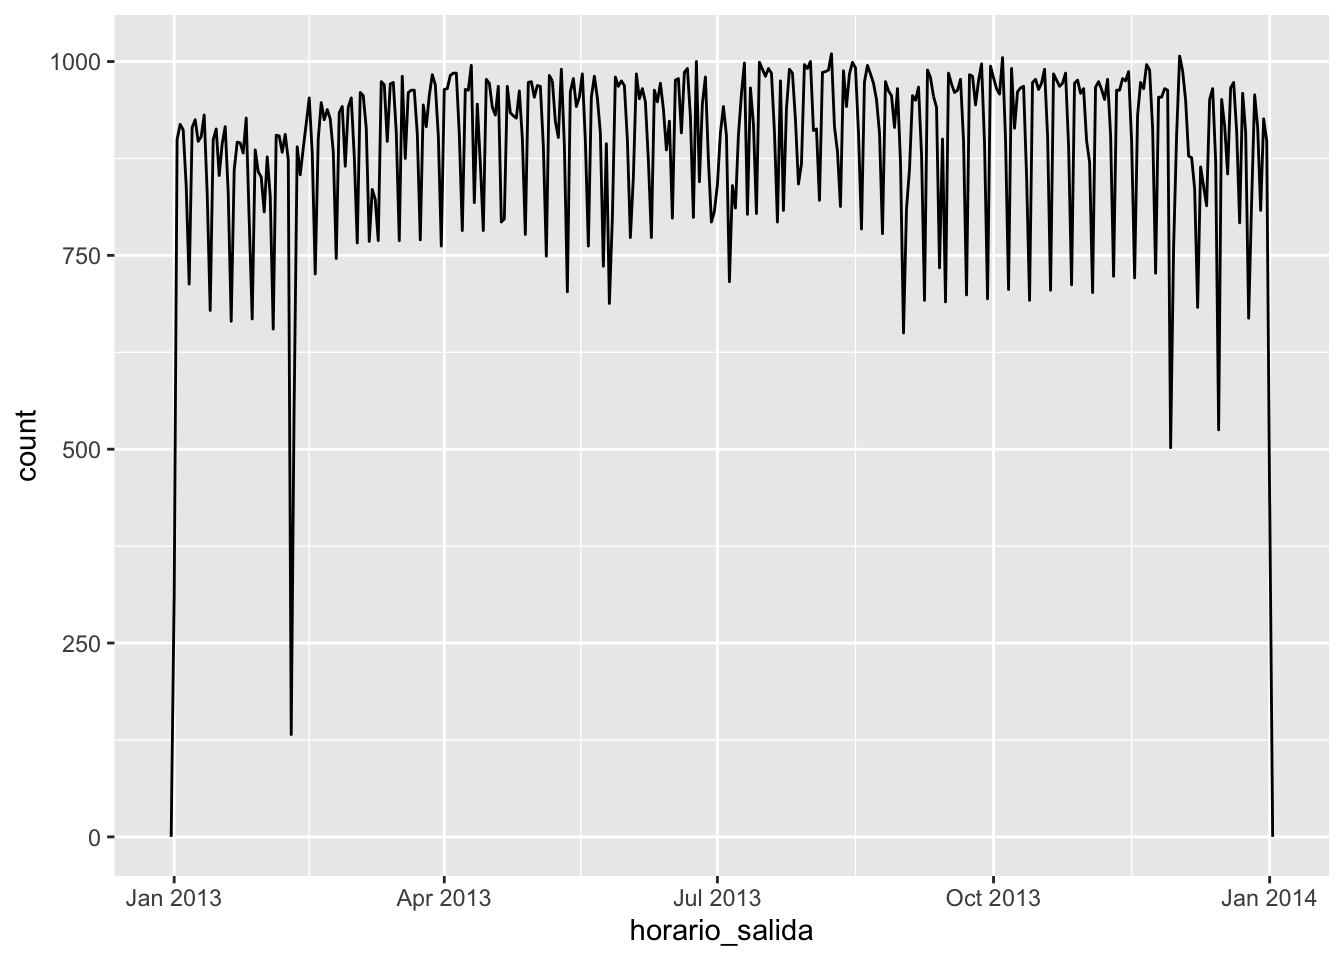
\includegraphics{Dinamica_poblacional_files/figure-latex/unnamed-chunk-23-1.pdf}

La tasa de transición de plántula a juvenil se reduce cuando el tamaño de la muestra es demasiado grande. En general, el tamaño de la muestra previa debe ser menos que el tamaño de muestra observado.

\hypertarget{intervalos-creuxedbles-de-lambda}{%
\section{\texorpdfstring{Intervalos creíbles de \(\lambda\)}{Intervalos creíbles de \textbackslash lambda}}\label{intervalos-creuxedbles-de-lambda}}

Obteniendo intervalos creíbles sobre la tasa de crecimiento asintótica, \(\lambda\), requiere simular matrices a partir de las distribuciones posteriores. Esto es algo complicado de hacer correctamente, y hemos escrito una función \texttt{raretrans::sim\_transitions()} para generar una lista de matrices simuladas dada la matriz observada y especificaciones previas.

\begin{Shaded}
\begin{Highlighting}[]
\FunctionTok{sim\_transitions}\NormalTok{(TF, N, }\AttributeTok{P =}\NormalTok{ RLT\_Tprior, }\AttributeTok{alpha =}\NormalTok{ alpha, }\AttributeTok{beta =}\NormalTok{ beta,}
                \AttributeTok{priorweight =} \FloatTok{0.5}\NormalTok{)}
\end{Highlighting}
\end{Shaded}

\begin{verbatim}
## [[1]]
##              [,1]         [,2]       [,3]
## [1,] 3.750857e-02 0.0009022215 0.28761593
## [2,] 5.621415e-01 0.7122223138 0.00351573
## [3,] 7.389564e-05 0.1731056616 0.94581372
\end{verbatim}

Ahora simulamos 5000 veces, calculamos el valor \(\lambda\) de cada
matriz y creamos un histograma de la distribución.

\begin{Shaded}
\begin{Highlighting}[]
\CommentTok{\#set.seed(8390278) \# make this part reproducible}
\NormalTok{alpha2 }\OtherTok{\textless{}{-}} \FunctionTok{matrix}\NormalTok{(}\FunctionTok{c}\NormalTok{(}\ConstantTok{NA\_real\_}\NormalTok{, }\ConstantTok{NA\_real\_}\NormalTok{, }\FloatTok{0.025}\NormalTok{,}
                  \ConstantTok{NA\_real\_}\NormalTok{, }\ConstantTok{NA\_real\_}\NormalTok{, }\ConstantTok{NA\_real\_}\NormalTok{,}
                  \ConstantTok{NA\_real\_}\NormalTok{, }\ConstantTok{NA\_real\_}\NormalTok{, }\ConstantTok{NA\_real\_}\NormalTok{), }\AttributeTok{nrow=}\DecValTok{3}\NormalTok{, }\AttributeTok{ncol =} \DecValTok{3}\NormalTok{, }\AttributeTok{byrow =} \ConstantTok{TRUE}\NormalTok{)}
\NormalTok{beta2 }\OtherTok{\textless{}{-}} \FunctionTok{matrix}\NormalTok{(}\FunctionTok{c}\NormalTok{(}\ConstantTok{NA\_real\_}\NormalTok{, }\ConstantTok{NA\_real\_}\NormalTok{, }\DecValTok{1}\NormalTok{,}
                  \ConstantTok{NA\_real\_}\NormalTok{, }\ConstantTok{NA\_real\_}\NormalTok{, }\ConstantTok{NA\_real\_}\NormalTok{,}
                  \ConstantTok{NA\_real\_}\NormalTok{, }\ConstantTok{NA\_real\_}\NormalTok{, }\ConstantTok{NA\_real\_}\NormalTok{), }\AttributeTok{nrow=}\DecValTok{3}\NormalTok{, }\AttributeTok{ncol =} \DecValTok{3}\NormalTok{, }\AttributeTok{byrow =} \ConstantTok{TRUE}\NormalTok{)}
\CommentTok{\# generar 5000 matrices basado en las previas de transciones y de fertilidades, el tamaño de muestra, en adición de los datos}
\NormalTok{RLT\_0}\FloatTok{.5} \OtherTok{\textless{}{-}} \FunctionTok{sim\_transitions}\NormalTok{(TF, N, }\AttributeTok{P =}\NormalTok{ RLT\_Tprior, }\AttributeTok{alpha =}\NormalTok{ alpha2, }\AttributeTok{beta =}\NormalTok{ beta2,}
                \AttributeTok{priorweight =} \FloatTok{0.5}\NormalTok{, }\AttributeTok{samples =} \DecValTok{5000}\NormalTok{)}
\CommentTok{\# extract the lambdas for each matrix}
\NormalTok{RLT\_0}\FloatTok{.5} \OtherTok{\textless{}{-}} \FunctionTok{tibble}\NormalTok{(}\AttributeTok{lposterior =} \FunctionTok{map\_dbl}\NormalTok{(RLT\_0}\FloatTok{.5}\NormalTok{, lambda)) }\CommentTok{\# convertir la lista en un tibble}
\FunctionTok{ggplot}\NormalTok{(}\AttributeTok{data =}\NormalTok{ RLT\_0}\FloatTok{.5}\NormalTok{,}
       \AttributeTok{mapping =} \FunctionTok{aes}\NormalTok{(}\AttributeTok{x =}\NormalTok{ lposterior)) }\SpecialCharTok{+} 
  \FunctionTok{geom\_histogram}\NormalTok{(}\AttributeTok{binwidth =} \FloatTok{0.01}\NormalTok{, }\AttributeTok{colour=}\StringTok{"white"}\NormalTok{) }\SpecialCharTok{+} 
\NormalTok{  rlt\_theme}
\end{Highlighting}
\end{Shaded}

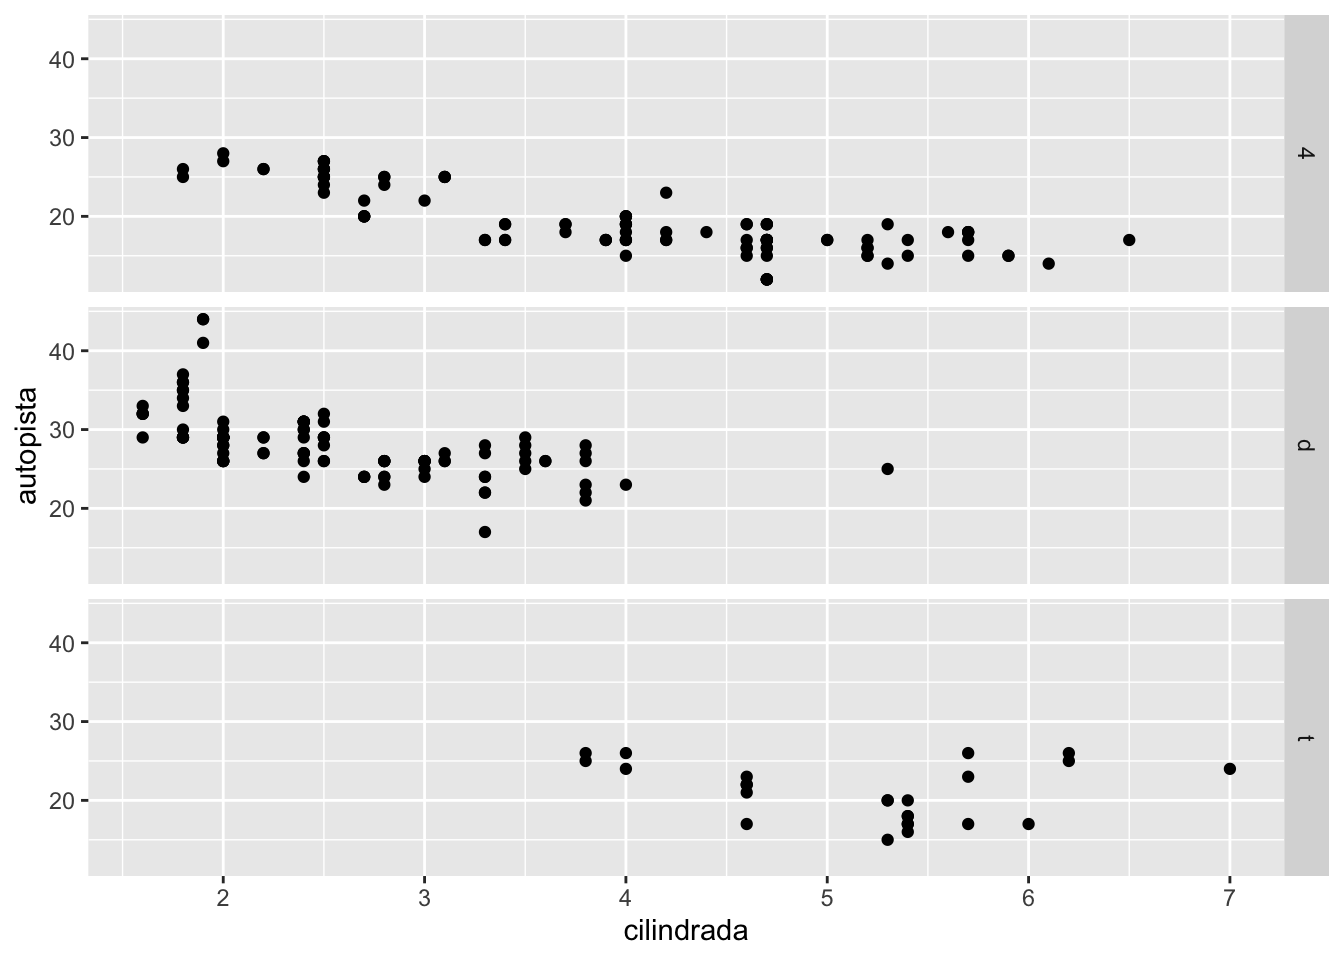
\includegraphics{Dinamica_poblacional_files/figure-latex/unnamed-chunk-25-1.pdf}

\hypertarget{detemrinar-si-el-lambda-es-significativamente-diferente-de-1}{%
\section{\texorpdfstring{Detemrinar si el \(\lambda\) es significativamente diferente de 1}{Detemrinar si el \textbackslash lambda es significativamente diferente de 1}}\label{detemrinar-si-el-lambda-es-significativamente-diferente-de-1}}

También podemos calcular algunas estadísticas de resumen. \texttt{pincrease} es el
probabilidad de que \(\lambda > 1\).

\begin{Shaded}
\begin{Highlighting}[]
\NormalTok{RLT\_0}\FloatTok{.5}\NormalTok{\_summary }\OtherTok{\textless{}{-}} \FunctionTok{summarize}\NormalTok{(RLT\_0}\FloatTok{.5}\NormalTok{,}
                             \AttributeTok{medianL =} \FunctionTok{median}\NormalTok{(lposterior),}
                             \AttributeTok{meanL =} \FunctionTok{mean}\NormalTok{(lposterior),}
                             \AttributeTok{lcl =} \FunctionTok{quantile}\NormalTok{(lposterior, }\AttributeTok{probs =} \FloatTok{0.025}\NormalTok{),}
                             \AttributeTok{ucl =} \FunctionTok{quantile}\NormalTok{(lposterior, }\AttributeTok{probs =} \FloatTok{0.975}\NormalTok{),}
                             \AttributeTok{pincrease =} \FunctionTok{sum}\NormalTok{(lposterior }\SpecialCharTok{\textgreater{}} \FloatTok{1.}\NormalTok{)}\SpecialCharTok{/}\FunctionTok{n}\NormalTok{())}
\NormalTok{knitr}\SpecialCharTok{::}\FunctionTok{kable}\NormalTok{(RLT\_0}\FloatTok{.5}\NormalTok{\_summary, }\AttributeTok{digits =} \DecValTok{2}\NormalTok{)}
\end{Highlighting}
\end{Shaded}

\begin{tabular}{r|r|r|r|r}
\hline
medianL & meanL & lcl & ucl & pincrease\\
\hline
0.96 & 0.96 & 0.87 & 1.03 & 0.14\\
\hline
\end{tabular}

\hypertarget{crecimiento-poblacional}{%
\chapter{Crecimiento Poblacional}\label{crecimiento-poblacional}}

Por: ???

\hypertarget{introducciuxf3n-al-crecimiento-poblacional}{%
\section{Introducción al crecimiento poblacional}\label{introducciuxf3n-al-crecimiento-poblacional}}

Ahora el primer paso es explicar a que \ldots..

\hypertarget{muxe9todos}{%
\section{Métodos}\label{muxe9todos}}

\hypertarget{elasticidad}{%
\chapter{Elasticidad}\label{elasticidad}}

\hypertarget{por-ernesto-mujica-y-elaine-gonzalez-1}{%
\section{Por: Ernesto Mujica y Elaine Gonzalez}\label{por-ernesto-mujica-y-elaine-gonzalez-1}}

\hypertarget{quuxe9-es-la-elasticidad}{%
\section{Qué es la Elasticidad}\label{quuxe9-es-la-elasticidad}}

\hypertarget{como-se-interpreta-la-eslaticidad}{%
\section{Como se interpreta la eslaticidad}\label{como-se-interpreta-la-eslaticidad}}

\hypertarget{como-se-calcula-la-eslasticidad}{%
\section{Como se calcula la eslasticidad}\label{como-se-calcula-la-eslasticidad}}

\hypertarget{limitaciones}{%
\section{Limitaciones}\label{limitaciones}}

\hypertarget{referencias-6}{%
\section{Referencias}\label{referencias-6}}

\hypertarget{dinuxe1mica-de-transiciones}{%
\chapter{Dinámica de transiciones}\label{dinuxe1mica-de-transiciones}}

Por: ???

\hypertarget{definiciones-de-dt}{%
\section{Definiciones de DT}\label{definiciones-de-dt}}

\hypertarget{cual-es-la-ventaja-de-la-dt}{%
\section{Cual es la ventaja de la DT}\label{cual-es-la-ventaja-de-la-dt}}

\hypertarget{como-se-calcula}{%
\section{Como se calcula}\label{como-se-calcula}}

\hypertarget{paquete-de-r-para-calcular-la-dt}{%
\section{Paquete de R para calcular la DT}\label{paquete-de-r-para-calcular-la-dt}}

\hypertarget{limitaciones-1}{%
\section{Limitaciones}\label{limitaciones-1}}

\hypertarget{referencias-7}{%
\section{Referencias}\label{referencias-7}}

\hypertarget{section}{%
\section{}\label{section}}

\hypertarget{metodos-de-simulaciones}{%
\chapter{Metodos de Simulaciones}\label{metodos-de-simulaciones}}

\hypertarget{introducciones-a-muxe9todos-de-simulaciones}{%
\section{Introducciones a métodos de simulaciones}\label{introducciones-a-muxe9todos-de-simulaciones}}

\hypertarget{ventaja-de-usar-simulaciones}{%
\section{Ventaja de usar simulaciones}\label{ventaja-de-usar-simulaciones}}

\hypertarget{ejemplo-simple-de-simulaciones}{%
\section{Ejemplo Simple de simulaciones}\label{ejemplo-simple-de-simulaciones}}

\hypertarget{elasticidad-no-lineal}{%
\chapter{Elasticidad no lineal}\label{elasticidad-no-lineal}}

\hypertarget{por-1}{%
\section{Por : ???}\label{por-1}}

\hypertarget{transfer-function}{%
\section{Transfer function}\label{transfer-function}}

\hypertarget{valor-bioluxf3gico}{%
\section{Valor biológico}\label{valor-bioluxf3gico}}

\hypertarget{muxe9todos-de-calculo}{%
\section{Métodos de calculo}\label{muxe9todos-de-calculo}}

\hypertarget{paquete-de-r-para-calcular-le-eslaticidad-no-lineal}{%
\section{Paquete de R para calcular le eslaticidad no lineal}\label{paquete-de-r-para-calcular-le-eslaticidad-no-lineal}}

\hypertarget{referencias-8}{%
\section{Referencias}\label{referencias-8}}

\hypertarget{comadre}{%
\chapter{COMADRE}\label{comadre}}

\begin{Shaded}
\begin{Highlighting}[]
\FunctionTok{library}\NormalTok{(Rcompadre)}
\FunctionTok{library}\NormalTok{(tidyverse)}
\FunctionTok{library}\NormalTok{(gt)}
\FunctionTok{library}\NormalTok{(kableExtra)}
\end{Highlighting}
\end{Shaded}

\begin{verbatim}
## 
## Attaching package: 'kableExtra'
\end{verbatim}

\begin{verbatim}
## The following object is masked from 'package:dplyr':
## 
##     group_rows
\end{verbatim}

Load your data from the website (e.g.:)
load(``/Users/user/Downloads/COMPADRE\_v.6.23.5.0.RData'')
index \textless- which(compadre\(metadata\)Family==``Orchidaceae'')
compadre\(metadata[index,] compadre\)mat{[}index{]}

\begin{Shaded}
\begin{Highlighting}[]
\FunctionTok{load}\NormalTok{(}\StringTok{"\textasciitilde{}/Dropbox/GitHub\_Dropbox\_Drive/GitHub/Taller\_Demo\_Peru/Taller\_Diagnostico\_Poblacional/COMPADRE\_v.6.23.5.0.RData"}\NormalTok{)}

\NormalTok{ALLSp}\OtherTok{=}\FunctionTok{as\_cdb}\NormalTok{(compadre)  }\CommentTok{\# the critical step was this part}


\NormalTok{index }\OtherTok{\textless{}{-}} \FunctionTok{which}\NormalTok{(ALLSp}\SpecialCharTok{$}\NormalTok{metadata}\SpecialCharTok{$}\NormalTok{Family}\SpecialCharTok{==}\StringTok{"Orchidaceae"}\NormalTok{) }
\FunctionTok{summary}\NormalTok{(ALLSp)}
\end{Highlighting}
\end{Shaded}

\begin{verbatim}
##     Length      Class       Mode 
##          1 CompadreDB         S4
\end{verbatim}

\begin{Shaded}
\begin{Highlighting}[]
\FunctionTok{names}\NormalTok{(ALLSp)}
\end{Highlighting}
\end{Shaded}

\begin{verbatim}
##  [1] "mat"                    "MatrixID"               "SpeciesAuthor"         
##  [4] "SpeciesAccepted"        "CommonName"             "Kingdom"               
##  [7] "Phylum"                 "Class"                  "Order"                 
## [10] "Family"                 "Genus"                  "Species"               
## [13] "Infraspecies"           "InfraspeciesType"       "OrganismType"          
## [16] "DicotMonoc"             "AngioGymno"             "Authors"               
## [19] "Journal"                "SourceType"             "OtherType"             
## [22] "YearPublication"        "DOI_ISBN"               "AdditionalSource"      
## [25] "StudyDuration"          "StudyStart"             "StudyEnd"              
## [28] "ProjectionInterval"     "MatrixCriteriaSize"     "MatrixCriteriaOntogeny"
## [31] "MatrixCriteriaAge"      "MatrixPopulation"       "NumberPopulations"     
## [34] "Lat"                    "Lon"                    "Altitude"              
## [37] "Country"                "Continent"              "Ecoregion"             
## [40] "StudiedSex"             "MatrixComposite"        "MatrixSeasonal"        
## [43] "MatrixTreatment"        "MatrixCaptivity"        "MatrixStartYear"       
## [46] "MatrixStartSeason"      "MatrixStartMonth"       "MatrixEndYear"         
## [49] "MatrixEndSeason"        "MatrixEndMonth"         "CensusType"            
## [52] "MatrixSplit"            "MatrixFec"              "Observations"          
## [55] "MatrixDimension"        "SurvivalIssue"          "_Database"             
## [58] "_PopulationStatus"      "_PublicationStatus"
\end{verbatim}

\begin{Shaded}
\begin{Highlighting}[]
\NormalTok{index\_O}\OtherTok{=}\NormalTok{ALLSp }\SpecialCharTok{\%\textgreater{}\%} 
 \FunctionTok{filter}\NormalTok{(Family }\SpecialCharTok{\%in\%} \FunctionTok{c}\NormalTok{(}\StringTok{"Orchidaceae"}\NormalTok{)) }\CommentTok{\# use small "compadre"}
\end{Highlighting}
\end{Shaded}

\begin{Shaded}
\begin{Highlighting}[]
\FunctionTok{unique}\NormalTok{(index\_O}\SpecialCharTok{$}\NormalTok{SpeciesAccepted)}
\end{Highlighting}
\end{Shaded}

\begin{verbatim}
##  [1] "Caladenia amonea"          "Caladenia argocalla"      
##  [3] "Caladenia clavigera"       "Caladenia elegans"        
##  [5] "Caladenia graniticola"     "Caladenia macroclavia"    
##  [7] "Caladenia oenochila"       "Caladenia rosella"        
##  [9] "Caladenia valida"          "Epipactis atrorubens"     
## [11] "Lepanthes rubripetala"     "Spathoglottis plicata"    
## [13] "Broughtonia cubensis"      "Cephalanthera longifolia" 
## [15] "Cleistes bifaria"          "Cypripedium calceolus"    
## [17] "Dendrophylax lindenii"     "Erycina crista-galli"     
## [19] "Lepanthes acuminata"       "Lepanthes caritensis"     
## [21] "Oncidium poikilostalix"    "Serapias cordigera"       
## [23] "Telipogon helleri"         "Aspasia principissa"      
## [25] "Guarianthe aurantiaca"     "Jacquiniella leucomelana" 
## [27] "Jacquiniella teretifolia"  "Lepanthes eltoroensis"    
## [29] "Lycaste aromatica"         "Tolumnia variegata"       
## [31] "Cleistesiopsis bifaria"    "Cleistesiopsis divaricata"
## [33] "Corallorhiza trifida"      "Cypripedium fasciculatum" 
## [35] "Cypripedium lentiginosum"  "Cypripedium parviflorum"  
## [37] "Dactylorhiza lapponica"    "Herminium monorchis"      
## [39] "Himantoglossum hircinum"   "Lepanthes rupestris"      
## [41] "Neotinea ustulata"         "Ophrys sphegodes"         
## [43] "Orchis purpurea"           "Platanthera hookeri"      
## [45] "Oeceoclades maculata"      "Brassavola cucullata"
\end{verbatim}

\begin{Shaded}
\begin{Highlighting}[]
\FunctionTok{names}\NormalTok{(index\_O)}
\end{Highlighting}
\end{Shaded}

\begin{verbatim}
##  [1] "mat"                    "MatrixID"               "SpeciesAuthor"         
##  [4] "SpeciesAccepted"        "CommonName"             "Kingdom"               
##  [7] "Phylum"                 "Class"                  "Order"                 
## [10] "Family"                 "Genus"                  "Species"               
## [13] "Infraspecies"           "InfraspeciesType"       "OrganismType"          
## [16] "DicotMonoc"             "AngioGymno"             "Authors"               
## [19] "Journal"                "SourceType"             "OtherType"             
## [22] "YearPublication"        "DOI_ISBN"               "AdditionalSource"      
## [25] "StudyDuration"          "StudyStart"             "StudyEnd"              
## [28] "ProjectionInterval"     "MatrixCriteriaSize"     "MatrixCriteriaOntogeny"
## [31] "MatrixCriteriaAge"      "MatrixPopulation"       "NumberPopulations"     
## [34] "Lat"                    "Lon"                    "Altitude"              
## [37] "Country"                "Continent"              "Ecoregion"             
## [40] "StudiedSex"             "MatrixComposite"        "MatrixSeasonal"        
## [43] "MatrixTreatment"        "MatrixCaptivity"        "MatrixStartYear"       
## [46] "MatrixStartSeason"      "MatrixStartMonth"       "MatrixEndYear"         
## [49] "MatrixEndSeason"        "MatrixEndMonth"         "CensusType"            
## [52] "MatrixSplit"            "MatrixFec"              "Observations"          
## [55] "MatrixDimension"        "SurvivalIssue"          "_Database"             
## [58] "_PopulationStatus"      "_PublicationStatus"
\end{verbatim}

\begin{Shaded}
\begin{Highlighting}[]
\NormalTok{index\_O}
\end{Highlighting}
\end{Shaded}

\begin{verbatim}
## A COM(P)ADRE database ('CompadreDB') object with 46 SPECIES and 647 MATRICES.
## 
## # A tibble: 647 x 59
##    mat        MatrixID SpeciesAuthor   SpeciesAccepted CommonName Kingdom Phylum
##    <list>        <int> <chr>           <chr>           <chr>      <chr>   <chr> 
##  1 <CompdrMt>   238285 Caladenia_amon~ Caladenia amon~ <NA>       Plantae Trach~
##  2 <CompdrMt>   238286 Caladenia_argo~ Caladenia argo~ <NA>       Plantae Trach~
##  3 <CompdrMt>   238287 Caladenia_clav~ Caladenia clav~ <NA>       Plantae Trach~
##  4 <CompdrMt>   238288 Caladenia_eleg~ Caladenia eleg~ <NA>       Plantae Trach~
##  5 <CompdrMt>   238289 Caladenia_gran~ Caladenia gran~ <NA>       Plantae Trach~
##  6 <CompdrMt>   238290 Caladenia_macr~ Caladenia macr~ <NA>       Plantae Trach~
##  7 <CompdrMt>   238291 Caladenia_oeno~ Caladenia oeno~ <NA>       Plantae Trach~
##  8 <CompdrMt>   238292 Caladenia_rose~ Caladenia rose~ <NA>       Plantae Trach~
##  9 <CompdrMt>   238293 Caladenia_vali~ Caladenia vali~ <NA>       Plantae Trach~
## 10 <CompdrMt>   238565 Epipactis_atro~ Epipactis atro~ Darkred h~ Plantae Trach~
## # i 637 more rows
## # i 52 more variables: Class <chr>, Order <chr>, Family <chr>, Genus <chr>,
## #   Species <chr>, Infraspecies <chr>, InfraspeciesType <chr>,
## #   OrganismType <chr>, DicotMonoc <chr>, AngioGymno <chr>, Authors <chr>,
## #   Journal <chr>, SourceType <chr>, OtherType <chr>, YearPublication <chr>,
## #   DOI_ISBN <chr>, AdditionalSource <chr>, StudyDuration <chr>,
## #   StudyStart <chr>, StudyEnd <chr>, ProjectionInterval <chr>, ...
\end{verbatim}

\hypertarget{how-many-unique-studies}{%
\section{How many unique studies?}\label{how-many-unique-studies}}

To know how long the studies were and be unique I need to select combinations of variables that nmake it unique.

\begin{Shaded}
\begin{Highlighting}[]
\FunctionTok{names}\NormalTok{(index\_O)}
\end{Highlighting}
\end{Shaded}

\begin{verbatim}
##  [1] "mat"                    "MatrixID"               "SpeciesAuthor"         
##  [4] "SpeciesAccepted"        "CommonName"             "Kingdom"               
##  [7] "Phylum"                 "Class"                  "Order"                 
## [10] "Family"                 "Genus"                  "Species"               
## [13] "Infraspecies"           "InfraspeciesType"       "OrganismType"          
## [16] "DicotMonoc"             "AngioGymno"             "Authors"               
## [19] "Journal"                "SourceType"             "OtherType"             
## [22] "YearPublication"        "DOI_ISBN"               "AdditionalSource"      
## [25] "StudyDuration"          "StudyStart"             "StudyEnd"              
## [28] "ProjectionInterval"     "MatrixCriteriaSize"     "MatrixCriteriaOntogeny"
## [31] "MatrixCriteriaAge"      "MatrixPopulation"       "NumberPopulations"     
## [34] "Lat"                    "Lon"                    "Altitude"              
## [37] "Country"                "Continent"              "Ecoregion"             
## [40] "StudiedSex"             "MatrixComposite"        "MatrixSeasonal"        
## [43] "MatrixTreatment"        "MatrixCaptivity"        "MatrixStartYear"       
## [46] "MatrixStartSeason"      "MatrixStartMonth"       "MatrixEndYear"         
## [49] "MatrixEndSeason"        "MatrixEndMonth"         "CensusType"            
## [52] "MatrixSplit"            "MatrixFec"              "Observations"          
## [55] "MatrixDimension"        "SurvivalIssue"          "_Database"             
## [58] "_PopulationStatus"      "_PublicationStatus"
\end{verbatim}

\begin{Shaded}
\begin{Highlighting}[]
\NormalTok{SPECIES\_O}\OtherTok{=}\NormalTok{index\_O }\SpecialCharTok{\%\textgreater{}\%} \FunctionTok{select}\NormalTok{(StudyStart, StudyEnd, SpeciesAccepted, YearPublication, Authors, DOI\_ISBN, OrganismType, MatrixPopulation,mat) }\SpecialCharTok{\%\textgreater{}\%} 
  \FunctionTok{group\_by}\NormalTok{(SpeciesAccepted, YearPublication, Authors, DOI\_ISBN, OrganismType, StudyStart, StudyEnd) }\SpecialCharTok{\%\textgreater{}\%} 
  \FunctionTok{summarize}\NormalTok{(}\AttributeTok{n\_populations =} \FunctionTok{length}\NormalTok{(}\FunctionTok{unique}\NormalTok{(MatrixPopulation))) }\SpecialCharTok{\%\textgreater{}\%} 
  \FunctionTok{arrange}\NormalTok{(}\FunctionTok{desc}\NormalTok{(n\_populations)) }\SpecialCharTok{\%\textgreater{}\%} 
  \FunctionTok{mutate}\NormalTok{(}\AttributeTok{StudyStart=}\FunctionTok{as.numeric}\NormalTok{(StudyStart)) }\SpecialCharTok{\%\textgreater{}\%} 
  \FunctionTok{mutate}\NormalTok{(}\AttributeTok{StudyEnd=}\FunctionTok{as.numeric}\NormalTok{(StudyEnd)) }\SpecialCharTok{\%\textgreater{}\%} 
  \FunctionTok{drop\_na}\NormalTok{(StudyStart, StudyEnd)}

\NormalTok{SPECIES\_O }\SpecialCharTok{\%\textgreater{}\%} \FunctionTok{kable}\NormalTok{()}
\end{Highlighting}
\end{Shaded}

\begin{tabular}{l|l|l|l|l|r|r|r}
\hline
SpeciesAccepted & YearPublication & Authors & DOI\_ISBN & OrganismType & StudyStart & StudyEnd & n\_populations\\
\hline
Lepanthes caritensis & 2018 & Crain; Tremblay; Ferguson & 10.1002/1438-390X.1002 & Epiphyte & 2010 & 2012 & 18\\
\hline
Epipactis atrorubens & 2017 & Hens; Pakanen; Jäkäläniemi; Tuomi; Kvist & 10.1016/j.biocon.2017.04.019 & Herbaceous perennial & 2000 & 2015 & 8\\
\hline
Lepanthes rubripetala & 2010 & Schödelbauerová; Tremblay; Kindlmann & 10.1007/s10531-009-9724-1 & Epiphyte & 1994 & 2007 & 8\\
\hline
Lepanthes rupestris & 2001 & Tremblay; Ackerman & 10.1006/bijl.2000.0485 & Herbaceous perennial & 1994 & 1996 & 7\\
\hline
Lepanthes rupestris & 2014 & Tremblay; McCarthy & 10.1371/journal.pone.0102859 & Herbaceous perennial & 1993 & 1996 & 7\\
\hline
Orchis purpurea & 2010 & Jacquemyns; Brys; Jongejans & 10.1890/08-2321.1 & Herbaceous perennial & 2002 & 2008 & 7\\
\hline
Lepanthes rubripetala & 2001 & Tremblay; Ackerman & 10.1006/bijl.2000.0485 & Epiphyte & 1994 & 1996 & 6\\
\hline
Lepanthes rubripetala & 2015 & Tremblay; Raventós; Ackerman; & 10.1093/aob/mcv031 & Epiphyte & 1994 & 1996 & 6\\
\hline
Neotinea ustulata & 2007 & Shefferson; Tali & 10.1111/j.1365-2745.2006.01195.x & Herbaceous perennial & 1993 & 2005 & 6\\
\hline
Serapias cordigera & 2014 & Pellegrino; Bellusci & 10.1111/boj.12204 & Herbaceous perennial & 1999 & 2012 & 6\\
\hline
Cephalanthera longifolia & 2012 & Shefferson; Kull; Tali; Kellett & 10.1890/ES11-00328.1 & Herbaceous perennial & 2002 & 2007 & 4\\
\hline
Cleistesiopsis bifaria & 1991 & Wells; Willems & 90-5103-068-1 & Herbaceous perennial & 1983 & 1990 & 4\\
\hline
Cypripedium calceolus & 2005 & Nicolè; Brzosko; Till-Bottraud & 10.1111/j.1365-2745.2005.01010.x & Herbaceous perennial & 1991 & 2000 & 4\\
\hline
Cypripedium fasciculatum & 2011 & Thorpe; Stanley; Kayne; Latham & NA & Herbaceous perennial & 1999 & 2007 & 4\\
\hline
Oeceoclades maculata & 2019 & Riverón-Giró; Raventós; Damon; García-González; Mújica & 10.1007/s10530-019-01945-7 & Herbaceous perennial & 2014 & 2016 & 4\\
\hline
Platanthera hookeri & 2007 & Reddoch; Reddoch & 10.3159/1095-5674(2007)134[369:PEOPHO]2.0.CO;2 & Herbaceous perennial & 1990 & 2005 & 4\\
\hline
Brassavola cucullata & 2020 & Ackerman; Tremblay; Pérez; Madden; Bechtold; Boeken & NA & Epiphyte & 2009 & 2014 & 3\\
\hline
Cypripedium calceolus & 2012 & Shefferson; Kull; Tali; Kellett & 10.1890/ES11-00328.1 & Herbaceous perennial & 2002 & 2007 & 3\\
\hline
Dactylorhiza lapponica & 2010 & Sletvold; Øien; Moen & 10.1016/j.biocon.2009.12.017 & Herbaceous perennial & 1990 & 2006 & 3\\
\hline
Lepanthes eltoroensis & 2001 & Tremblay; Ackerman & 10.1006/bijl.2000.0485 & Epiphyte & 1994 & 1996 & 3\\
\hline
Cleistes bifaria & 2006 & Gregg; Kéry & 10.1016/j.biocon.2005.09.044 & Herbaceous perennial & 1986 & 1996 & 2\\
\hline
Cypripedium calceolus & 2010 & García; Goñi; Guzman & 10.1111/j.1523-1739.2010.01466.x & Herbaceous perennial & 1994 & 2002 & 2\\
\hline
Erycina crista-galli & 2007 & Mondragón; Maldonado; Aguilar-Santelises & 10.1111/boj.12204 & Epiphyte & 2004 & 2005 & 2\\
\hline
Jacquiniella leucomelana & 2009 & Winkler; Hülber; Hietz & 10.1093/aob/mcp188 & Epiphyte & 2002 & 2005 & 2\\
\hline
Jacquiniella teretifolia & 2009 & Winkler; Hülber; Hietz & 10.1093/aob/mcp188 & Epiphyte & 2002 & 2005 & 2\\
\hline
Lepanthes caritensis & 1997 & Tremblay & NA & Epiphyte & 1994 & 1996 & 2\\
\hline
Lycaste aromatica & 2009 & Winkler; Hülber; Hietz & 10.1093/aob/mcp188 & Epiphyte & 2002 & 2005 & 2\\
\hline
Aspasia principissa & 2006 & Zotz; Schmidt & 10.1016/j.biocon.2005.07.022 & Epiphyte & 1997 & 2004 & 1\\
\hline
Broughtonia cubensis & 2015 & Raventós; Gonzalez; Mújica; Bonet & 10.1111/btp.12231 & Epiphyte & 2006 & 2010 & 1\\
\hline
Caladenia amonea & 2009 & Tremblay; Pérez; Larcombe; Brown; Quarmby; Bickerton; French; Bould & 10.1071/BT08167 & Epiphyte & 1996 & 2007 & 1\\
\hline
Caladenia argocalla & 2009 & Tremblay; Pérez; Larcombe; Brown; Quarmby; Bickerton; French; Bould & 10.1071/BT08167 & Epiphyte & 1996 & 2007 & 1\\
\hline
Caladenia clavigera & 2009 & Tremblay; Pérez; Larcombe; Brown; Quarmby; Bickerton; French; Bould & 10.1071/BT08167 & Epiphyte & 1996 & 2007 & 1\\
\hline
Caladenia elegans & 2009 & Tremblay; Pérez; Larcombe; Brown; Quarmby; Bickerton; French; Bould & 10.1071/BT08167 & Epiphyte & 1996 & 2007 & 1\\
\hline
Caladenia graniticola & 2009 & Tremblay; Pérez; Larcombe; Brown; Quarmby; Bickerton; French; Bould & 10.1071/BT08167 & Epiphyte & 1996 & 2007 & 1\\
\hline
Caladenia macroclavia & 2009 & Tremblay; Pérez; Larcombe; Brown; Quarmby; Bickerton; French; Bould & 10.1071/BT08167 & Epiphyte & 1996 & 2007 & 1\\
\hline
Caladenia oenochila & 2009 & Tremblay; Pérez; Larcombe; Brown; Quarmby; Bickerton; French; Bould & 10.1071/BT08167 & Epiphyte & 1996 & 2007 & 1\\
\hline
Caladenia rosella & 2009 & Tremblay; Pérez; Larcombe; Brown; Quarmby; Bickerton; French; Bould & 10.1071/BT08167 & Epiphyte & 1996 & 2007 & 1\\
\hline
Caladenia valida & 2009 & Tremblay; Pérez; Larcombe; Brown; Quarmby; Bickerton; French; Bould & 10.1071/BT08167 & Epiphyte & 1996 & 2007 & 1\\
\hline
Cleistesiopsis divaricata & 1991 & Wells; Willems & 90-5103-068-1 & Herbaceous perennial & 1983 & 1990 & 1\\
\hline
Corallorhiza trifida & 2009 & Iriondo; Giménez-Benavides; Albert; Lozano; Escudero & 978-84-8014-746-0 & Herbaceous perennial & 2001 & 2004 & 1\\
\hline
Cypripedium parviflorum & 2014 & Shefferson; Warren II; Pulliam & 10.1111/1365-2745.12281 & Herbaceous perennial & 1994 & 2012 & 1\\
\hline
Dactylorhiza lapponica & 2013 & Sletvold; Dahlgren; Øien; Moen; Ehrlén & 10.1111/gcb.12167 & Herbaceous perennial & 1981 & 2010 & 1\\
\hline
Dendrophylax lindenii & 2015 & Raventós; Gonzalez; Mújica; Bonet & 10.1111/btp.12231 & Epiphyte & 2006 & 2010 & 1\\
\hline
Epipactis atrorubens & 2011 & Jäkäläniemi; Crone; Närhi; Tuomi & 10.1890/10-1957.1 & Herbaceous perennial & 2000 & 2008 & 1\\
\hline
Guarianthe aurantiaca & 2009 & Mondragón & 10.1111/j.1442-1984.2009.00230.x & Epiphyte & 2004 & 2006 & 1\\
\hline
Herminium monorchis & 1998 & Wells; Rothery; Cox; Bamford & 10.1111/j.1095-8339.1998.tb02514.x & Herbaceous perennial & 1966 & 1995 & 1\\
\hline
Himantoglossum hircinum & 2006 & Pfeifer; Wiegand; Heinrich; Jetschke & 10.1111/j.1365-2664.2006.01148.x & Herbaceous perennial & 1976 & 2001 & 1\\
\hline
Lepanthes acuminata & 2018 & Raventós; García-González; Riverón-Giró; Damon & 10.1080/17550874.2018.1444110 & Epiphyte & 2013 & 2015 & 1\\
\hline
Oncidium poikilostalix & 2017 & García-González; Damon; Raventós; Riverón-Giró; Mújica; Solís-Montero & 10.1080/17550874.2017.1315840 & Epiphyte & 2013 & 2015 & 1\\
\hline
Oncidium poikilostalix & 2018 & Raventós; García-González; Riverón-Giró; Damon & 10.1080/17550874.2018.1444110 & Epiphyte & 2013 & 2015 & 1\\
\hline
Ophrys sphegodes & 1991 & Wells; Willems & 90-5103-068-1 & Herbaceous perennial & 1983 & 1990 & 1\\
\hline
Spathoglottis plicata & 2017 & Falcón; Ackerman; Tremblay & 10.1007/s10530-016-1318-8 & Herbaceous perennial & 2009 & 2011 & 1\\
\hline
Telipogon helleri & 2018 & Raventós; García-González; Riverón-Giró; Damon & 10.1080/17550874.2018.1444110 & Epiphyte & 2013 & 2015 & 1\\
\hline
Tolumnia variegata & 1993 & Calvo & 10.2307/1940473 & Epiphyte & 1988 & 1990 & 1\\
\hline
\end{tabular}

\begin{Shaded}
\begin{Highlighting}[]
\FunctionTok{write\_csv}\NormalTok{(SPECIES\_O, }\StringTok{"Species\_O.csv"}\NormalTok{)}
\end{Highlighting}
\end{Shaded}

\begin{Shaded}
\begin{Highlighting}[]
\NormalTok{SPECIES\_O}\SpecialCharTok{$}\NormalTok{SpeciesAccepted }\OtherTok{\textless{}{-}} \FunctionTok{fct\_reorder}\NormalTok{(SPECIES\_O}\SpecialCharTok{$}\NormalTok{SpeciesAccepted, SPECIES\_O}\SpecialCharTok{$}\NormalTok{StudyStart, }\AttributeTok{.desc =} \ConstantTok{FALSE}\NormalTok{)}

\FunctionTok{ggplot}\NormalTok{(SPECIES\_O, }\FunctionTok{aes}\NormalTok{(SpeciesAccepted, }\AttributeTok{color=}\NormalTok{OrganismType))}\SpecialCharTok{+}
  \FunctionTok{geom\_linerange}\NormalTok{(}\FunctionTok{aes}\NormalTok{(}\AttributeTok{x=}\NormalTok{ SpeciesAccepted  , }\AttributeTok{ymin=}\NormalTok{StudyStart, }\AttributeTok{ymax=}\NormalTok{StudyEnd))}\SpecialCharTok{+}
  \FunctionTok{coord\_flip}\NormalTok{()}\SpecialCharTok{+}
  \FunctionTok{theme}\NormalTok{(}\AttributeTok{legend.position =} \FunctionTok{c}\NormalTok{(}\FloatTok{0.2}\NormalTok{, }\FloatTok{0.8}\NormalTok{))}\SpecialCharTok{+}
  \FunctionTok{theme}\NormalTok{(}\AttributeTok{axis.text.x =} \FunctionTok{element\_text}\NormalTok{(}\AttributeTok{color =} \StringTok{"grey20"}\NormalTok{, }\AttributeTok{size =} \DecValTok{9}\NormalTok{, }\AttributeTok{angle =} \DecValTok{90}\NormalTok{, }\AttributeTok{hjust =}\NormalTok{ .}\DecValTok{5}\NormalTok{, }\AttributeTok{vjust =}\NormalTok{ .}\DecValTok{5}\NormalTok{, }\AttributeTok{face =} \StringTok{"plain"}\NormalTok{),}
        \AttributeTok{axis.text.y =} \FunctionTok{element\_text}\NormalTok{(}\AttributeTok{color =} \StringTok{"grey20"}\NormalTok{, }\AttributeTok{size =} \DecValTok{7}\NormalTok{, }\AttributeTok{angle =} \DecValTok{0}\NormalTok{, }\AttributeTok{hjust =} \DecValTok{1}\NormalTok{, }\AttributeTok{vjust =} \DecValTok{0}\NormalTok{, }\AttributeTok{face =} \StringTok{"plain"}\NormalTok{),  }
        \AttributeTok{axis.title.x =} \FunctionTok{element\_text}\NormalTok{(}\AttributeTok{color =} \StringTok{"grey20"}\NormalTok{, }\AttributeTok{size =} \DecValTok{12}\NormalTok{, }\AttributeTok{angle =} \DecValTok{0}\NormalTok{, }\AttributeTok{hjust =}\NormalTok{ .}\DecValTok{5}\NormalTok{, }\AttributeTok{vjust =} \DecValTok{0}\NormalTok{, }\AttributeTok{face =} \StringTok{"plain"}\NormalTok{),}
        \AttributeTok{axis.title.y =} \FunctionTok{element\_text}\NormalTok{(}\AttributeTok{color =} \StringTok{"grey20"}\NormalTok{, }\AttributeTok{size =} \DecValTok{12}\NormalTok{, }\AttributeTok{angle =} \DecValTok{90}\NormalTok{, }\AttributeTok{hjust =}\NormalTok{ .}\DecValTok{5}\NormalTok{, }\AttributeTok{vjust =}\NormalTok{ .}\DecValTok{5}\NormalTok{, }\AttributeTok{face =} \StringTok{"plain"}\NormalTok{))}\SpecialCharTok{+}
  \FunctionTok{ylab}\NormalTok{(}\StringTok{""}\NormalTok{)}\SpecialCharTok{+}
  \FunctionTok{xlab}\NormalTok{(}\StringTok{""}\NormalTok{)}
\end{Highlighting}
\end{Shaded}

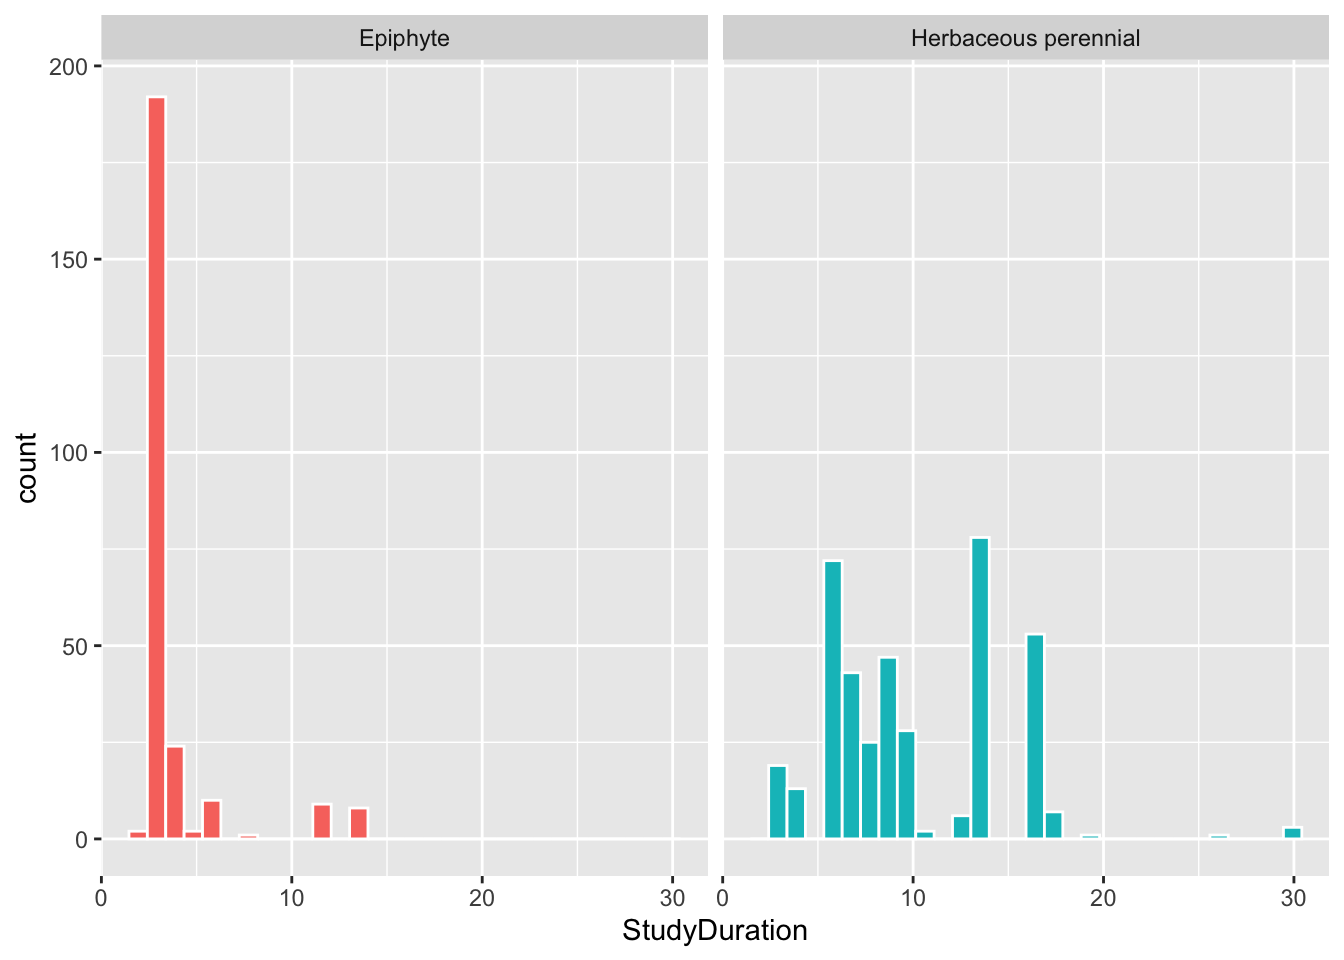
\includegraphics{Dinamica_poblacional_files/figure-latex/unnamed-chunk-32-1.pdf}

\begin{Shaded}
\begin{Highlighting}[]
\NormalTok{index\_O}\OtherTok{=}\NormalTok{index\_O }\SpecialCharTok{\%\textgreater{}\%} 
  \FunctionTok{mutate}\NormalTok{(}\AttributeTok{StudyDuration=}\FunctionTok{as.numeric}\NormalTok{(StudyDuration))}

\FunctionTok{table}\NormalTok{(index\_O}\SpecialCharTok{$}\NormalTok{StudyDuration)}
\end{Highlighting}
\end{Shaded}

\begin{verbatim}
## 
##   2   3   4   5   6   7   8   9  10  11  12  13  14  16  17  19  26  30 
##   2 211  37   2  82  43  26  47  28   2   9   6  86  53   7   1   1   3
\end{verbatim}

\begin{Shaded}
\begin{Highlighting}[]
\FunctionTok{table}\NormalTok{(index\_O}\SpecialCharTok{$}\NormalTok{OrganismType)}
\end{Highlighting}
\end{Shaded}

\begin{verbatim}
## 
##             Epiphyte Herbaceous perennial 
##                  248                  399
\end{verbatim}

\begin{Shaded}
\begin{Highlighting}[]
\FunctionTok{ggplot}\NormalTok{(index\_O, }\FunctionTok{aes}\NormalTok{(StudyDuration, }\AttributeTok{fill=}\NormalTok{OrganismType))}\SpecialCharTok{+}
         \FunctionTok{geom\_histogram}\NormalTok{(}\AttributeTok{colour=}\StringTok{"white"}\NormalTok{)}\SpecialCharTok{+}
  \FunctionTok{facet\_wrap}\NormalTok{(}\SpecialCharTok{\textasciitilde{}}\NormalTok{OrganismType)}\SpecialCharTok{+}
  \FunctionTok{theme}\NormalTok{(}\AttributeTok{legend.position =} \StringTok{"none"}\NormalTok{)}
\end{Highlighting}
\end{Shaded}

\begin{verbatim}
## `stat_bin()` using `bins = 30`. Pick better value with `binwidth`.
\end{verbatim}

\begin{verbatim}
## Warning: Removed 1 rows containing non-finite values (`stat_bin()`).
\end{verbatim}

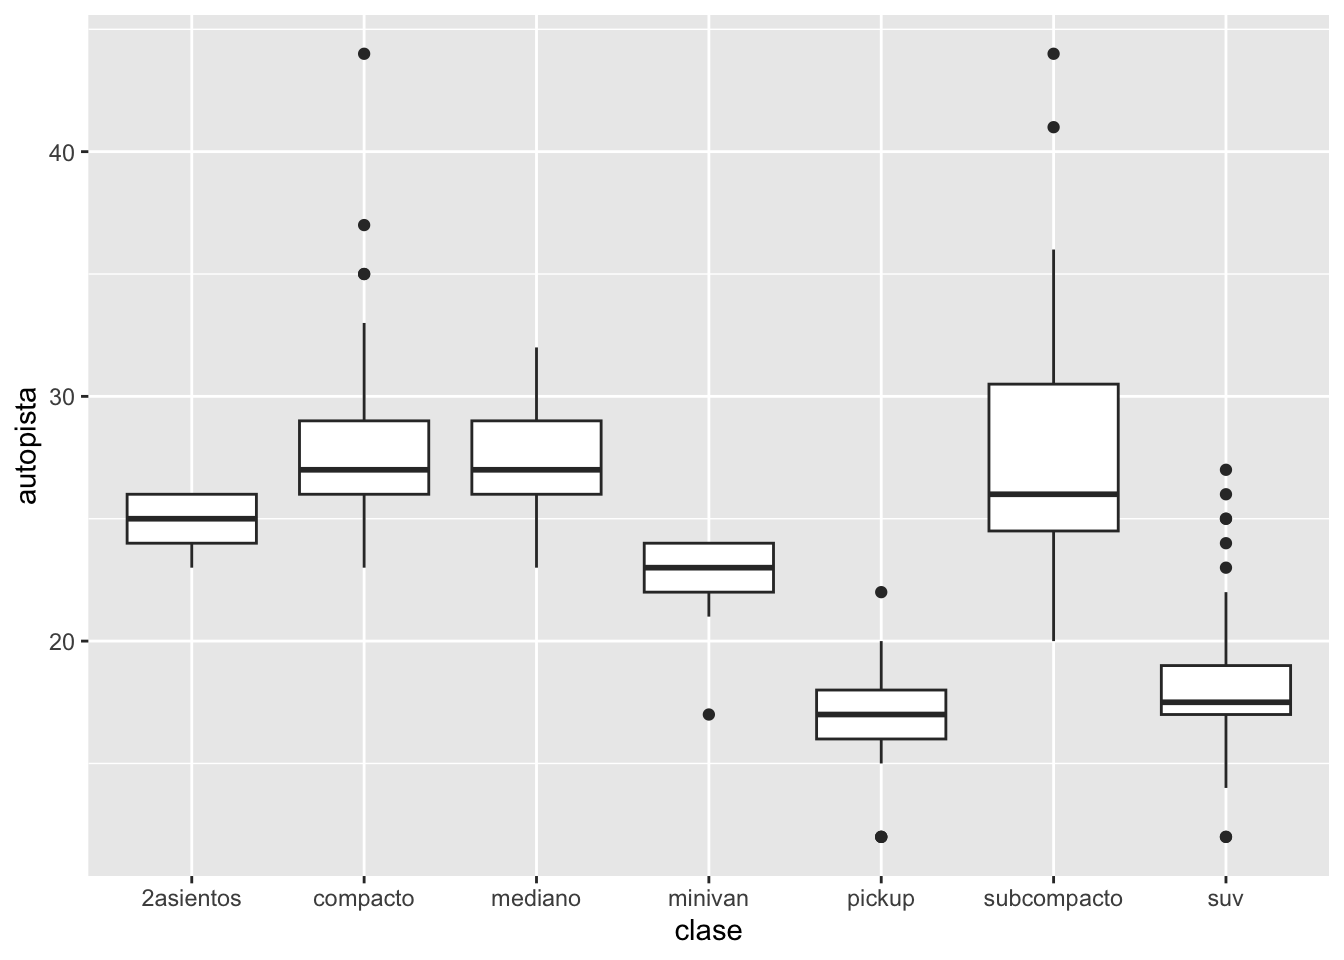
\includegraphics{Dinamica_poblacional_files/figure-latex/unnamed-chunk-33-1.pdf}

\begin{Shaded}
\begin{Highlighting}[]
\FunctionTok{ggsave}\NormalTok{(}\StringTok{"Duración\_Epi\_Ter.pdf"}\NormalTok{)}
\end{Highlighting}
\end{Shaded}

\begin{verbatim}
## Saving 6.5 x 4.5 in image
## `stat_bin()` using `bins = 30`. Pick better value with `binwidth`.
\end{verbatim}

\begin{verbatim}
## Warning: Removed 1 rows containing non-finite values (`stat_bin()`).
\end{verbatim}

\begin{Shaded}
\begin{Highlighting}[]
\FunctionTok{plot}\NormalTok{(index\_O}\SpecialCharTok{$}\NormalTok{Lon,index\_O}\SpecialCharTok{$}\NormalTok{Lat,}\AttributeTok{main =} \StringTok{"Location"}\NormalTok{)}
\end{Highlighting}
\end{Shaded}

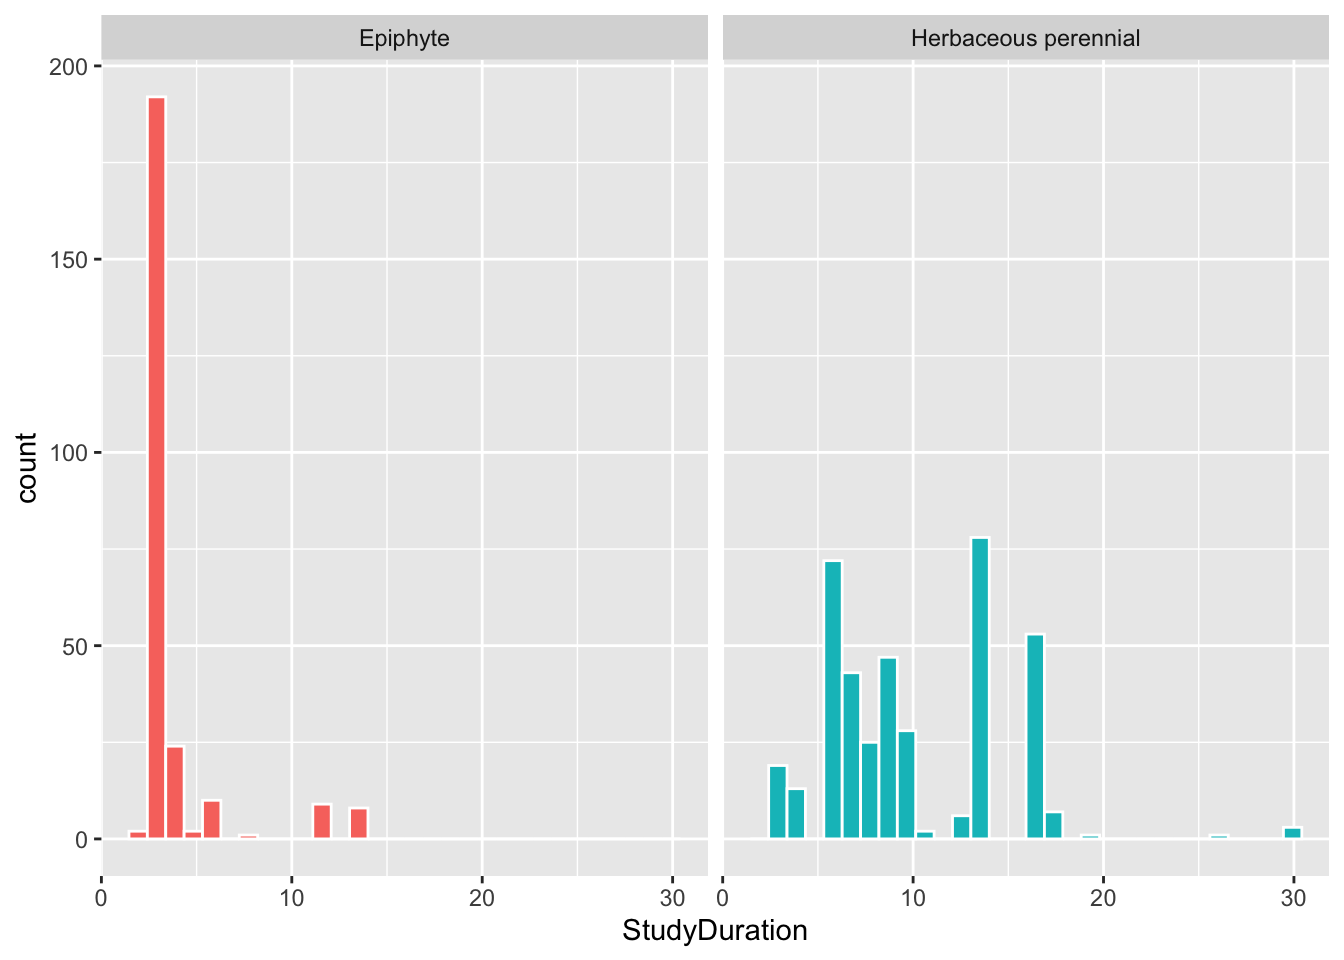
\includegraphics{Dinamica_poblacional_files/figure-latex/unnamed-chunk-34-1.pdf}

Getting the whole database for orchids

\begin{Shaded}
\begin{Highlighting}[]
\NormalTok{index }\OtherTok{\textless{}{-}} \FunctionTok{which}\NormalTok{(compadre}\SpecialCharTok{$}\NormalTok{metadata}\SpecialCharTok{$}\NormalTok{Family}\SpecialCharTok{==}\StringTok{"Orchidaceae"}\NormalTok{) }
\FunctionTok{names}\NormalTok{(Compadre)}
\end{Highlighting}
\end{Shaded}

\begin{verbatim}
##  [1] "mat"                    "SpeciesAuthor"          "SpeciesAccepted"       
##  [4] "CommonName"             "Genus"                  "Family"                
##  [7] "Order"                  "Class"                  "Phylum"                
## [10] "Kingdom"                "OrganismType"           "DicotMonoc"            
## [13] "AngioGymno"             "Authors"                "Journal"               
## [16] "YearPublication"        "DOI_ISBN"               "AdditionalSource"      
## [19] "StudyDuration"          "StudyStart"             "StudyEnd"              
## [22] "ProjectionInterval"     "NumberPopulations"      "MatrixCriteriaSize"    
## [25] "MatrixCriteriaOntogeny" "MatrixCriteriaAge"      "MatrixPopulation"      
## [28] "Lat"                    "Lon"                    "Altitude"              
## [31] "Country"                "Continent"              "Ecoregion"             
## [34] "StudiedSex"             "MatrixComposite"        "MatrixTreatment"       
## [37] "MatrixCaptivity"        "MatrixStartYear"        "MatrixStartSeason"     
## [40] "MatrixStartMonth"       "MatrixEndYear"          "MatrixEndSeason"       
## [43] "MatrixEndMonth"         "MatrixSplit"            "MatrixFec"             
## [46] "Observation"            "MatrixDimension"        "SurvivalIssue"         
## [49] "AnnualPeriodicity"
\end{verbatim}

\begin{Shaded}
\begin{Highlighting}[]
\FunctionTok{subset}\NormalTok{(index\_O, Family }\SpecialCharTok{==}\StringTok{"Orchidaceae"}  \SpecialCharTok{\&}
\NormalTok{             MatrixDimension }\SpecialCharTok{\textgreater{}}\DecValTok{2}\NormalTok{)}
\end{Highlighting}
\end{Shaded}

\begin{verbatim}
## A COM(P)ADRE database ('CompadreDB') object with 46 SPECIES and 647 MATRICES.
## 
## # A tibble: 647 x 59
##    mat        MatrixID SpeciesAuthor   SpeciesAccepted CommonName Kingdom Phylum
##    <list>        <int> <chr>           <chr>           <chr>      <chr>   <chr> 
##  1 <CompdrMt>   238285 Caladenia_amon~ Caladenia amon~ <NA>       Plantae Trach~
##  2 <CompdrMt>   238286 Caladenia_argo~ Caladenia argo~ <NA>       Plantae Trach~
##  3 <CompdrMt>   238287 Caladenia_clav~ Caladenia clav~ <NA>       Plantae Trach~
##  4 <CompdrMt>   238288 Caladenia_eleg~ Caladenia eleg~ <NA>       Plantae Trach~
##  5 <CompdrMt>   238289 Caladenia_gran~ Caladenia gran~ <NA>       Plantae Trach~
##  6 <CompdrMt>   238290 Caladenia_macr~ Caladenia macr~ <NA>       Plantae Trach~
##  7 <CompdrMt>   238291 Caladenia_oeno~ Caladenia oeno~ <NA>       Plantae Trach~
##  8 <CompdrMt>   238292 Caladenia_rose~ Caladenia rose~ <NA>       Plantae Trach~
##  9 <CompdrMt>   238293 Caladenia_vali~ Caladenia vali~ <NA>       Plantae Trach~
## 10 <CompdrMt>   238565 Epipactis_atro~ Epipactis atro~ Darkred h~ Plantae Trach~
## # i 637 more rows
## # i 52 more variables: Class <chr>, Order <chr>, Family <chr>, Genus <chr>,
## #   Species <chr>, Infraspecies <chr>, InfraspeciesType <chr>,
## #   OrganismType <chr>, DicotMonoc <chr>, AngioGymno <chr>, Authors <chr>,
## #   Journal <chr>, SourceType <chr>, OtherType <chr>, YearPublication <chr>,
## #   DOI_ISBN <chr>, AdditionalSource <chr>, StudyDuration <dbl>,
## #   StudyStart <chr>, StudyEnd <chr>, ProjectionInterval <chr>, ...
\end{verbatim}

\begin{Shaded}
\begin{Highlighting}[]
\FunctionTok{subset}\NormalTok{(index\_O,DicotMonoc }\SpecialCharTok{==} \StringTok{"Eudicot"} \SpecialCharTok{\&} 
\NormalTok{              Country }\SpecialCharTok{\%in\%} \FunctionTok{c}\NormalTok{(}\StringTok{"USA"}\NormalTok{, }\StringTok{"CAN"}\NormalTok{) }\SpecialCharTok{\&} 
\NormalTok{              MatrixDimension }\SpecialCharTok{\textgreater{}} \DecValTok{2}\NormalTok{)}
\end{Highlighting}
\end{Shaded}

\begin{verbatim}
## A COM(P)ADRE database ('CompadreDB') object with 0 SPECIES and 0 MATRICES.
## 
## # A tibble: 0 x 59
## # i 59 variables: mat <list>, MatrixID <int>, SpeciesAuthor <chr>,
## #   SpeciesAccepted <chr>, CommonName <chr>, Kingdom <chr>, Phylum <chr>,
## #   Class <chr>, Order <chr>, Family <chr>, Genus <chr>, Species <chr>,
## #   Infraspecies <chr>, InfraspeciesType <chr>, OrganismType <chr>,
## #   DicotMonoc <chr>, AngioGymno <chr>, Authors <chr>, Journal <chr>,
## #   SourceType <chr>, OtherType <chr>, YearPublication <chr>, DOI_ISBN <chr>,
## #   AdditionalSource <chr>, StudyDuration <dbl>, StudyStart <chr>, ...
\end{verbatim}

\begin{Shaded}
\begin{Highlighting}[]
\CommentTok{\#cdb\_compare(index\_O,x)}


\NormalTok{x }\OtherTok{\textless{}{-}} \FunctionTok{subset}\NormalTok{(index\_O,Family }\SpecialCharTok{==} \StringTok{"Orchidaceae"}\NormalTok{)}

\NormalTok{x\_OT}\OtherTok{=}\NormalTok{x }\SpecialCharTok{\%\textgreater{}\%} 
  \FunctionTok{group\_by}\NormalTok{(OrganismType)}
\end{Highlighting}
\end{Shaded}

\begin{Shaded}
\begin{Highlighting}[]
\CommentTok{\#Orchids\_New=as\_cdb(index)}
\CommentTok{\#compadre$mat[index]}

\NormalTok{Compadre\_flagged }\OtherTok{\textless{}{-}} \FunctionTok{cdb\_flag}\NormalTok{(index\_O)}

\NormalTok{x }\OtherTok{\textless{}{-}} \FunctionTok{subset}\NormalTok{(Compadre\_flagged, check\_NA\_A }\SpecialCharTok{==} \ConstantTok{FALSE} \SpecialCharTok{\&}\NormalTok{ check\_ergodic }\SpecialCharTok{==} \ConstantTok{TRUE}\NormalTok{)}

\NormalTok{lambdaVals }\OtherTok{\textless{}{-}} \FunctionTok{sapply}\NormalTok{(}\FunctionTok{matA}\NormalTok{(x), popdemo}\SpecialCharTok{::}\NormalTok{eigs, }\AttributeTok{what=}\StringTok{"lambda"}\NormalTok{)}
\FunctionTok{summary}\NormalTok{(lambdaVals)}
\end{Highlighting}
\end{Shaded}

\begin{verbatim}
##    Min. 1st Qu.  Median    Mean 3rd Qu.    Max. 
##  0.3888  0.9635  0.9973  0.9944  1.0232  1.7760
\end{verbatim}

\begin{Shaded}
\begin{Highlighting}[]
\FunctionTok{hist}\NormalTok{(lambdaVals, }\AttributeTok{main =} \StringTok{"Lambda values"}\NormalTok{)}
\end{Highlighting}
\end{Shaded}

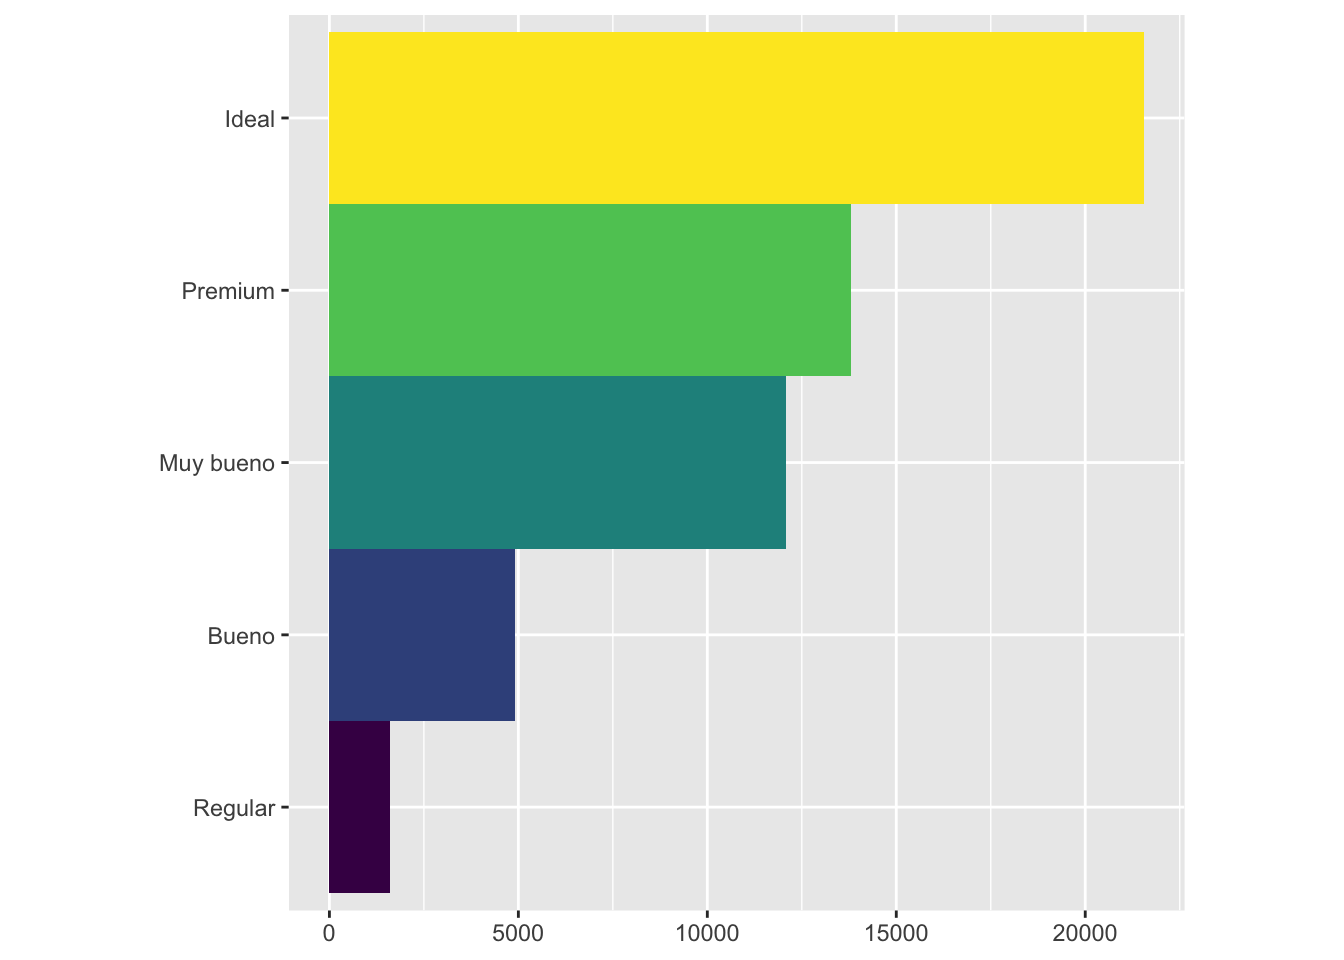
\includegraphics{Dinamica_poblacional_files/figure-latex/unnamed-chunk-36-1.pdf}

\begin{Shaded}
\begin{Highlighting}[]
\FunctionTok{library}\NormalTok{(purrr)}
\NormalTok{lambdaVals1 }\OtherTok{\textless{}{-}} \FunctionTok{map\_dbl}\NormalTok{(}\FunctionTok{matA}\NormalTok{(x), }\SpecialCharTok{\textasciitilde{}}\NormalTok{popdemo}\SpecialCharTok{::}\FunctionTok{eigs}\NormalTok{(.x, }\AttributeTok{what=}\StringTok{"lambda"}\NormalTok{))}
 
 
\CommentTok{\#Or with popbio, which avoids some warning messages…}
\NormalTok{lambdaVals2 }\OtherTok{\textless{}{-}} \FunctionTok{map\_dbl}\NormalTok{(}\FunctionTok{matA}\NormalTok{(x), }\SpecialCharTok{\textasciitilde{}}\NormalTok{popbio}\SpecialCharTok{::}\FunctionTok{lambda}\NormalTok{(.x))}
\end{Highlighting}
\end{Shaded}

\begin{Shaded}
\begin{Highlighting}[]
\NormalTok{x2}\OtherTok{=}\NormalTok{x }\SpecialCharTok{\%\textgreater{}\%} 
  \FunctionTok{mutate}\NormalTok{(}\AttributeTok{OrganismType =} \FunctionTok{case\_when}\NormalTok{(}
\NormalTok{    Genus }\SpecialCharTok{==}  \StringTok{"Caladenia"} \SpecialCharTok{\&}\NormalTok{ OrganismType }\SpecialCharTok{==} \StringTok{"Epiphyte"} \SpecialCharTok{\textasciitilde{}} \StringTok{"Herbaceous perennial"}\NormalTok{,}
    \ConstantTok{TRUE} \SpecialCharTok{\textasciitilde{}}\NormalTok{ OrganismType}
\NormalTok{  ))}

\NormalTok{epi}\OtherTok{=}\NormalTok{x2 }\SpecialCharTok{\%\textgreater{}\%} 
  \FunctionTok{filter}\NormalTok{(OrganismType}\SpecialCharTok{==}\StringTok{"Epiphyte"}\NormalTok{)}

\NormalTok{terr}\OtherTok{=}\NormalTok{x2 }\SpecialCharTok{\%\textgreater{}\%} 
  \FunctionTok{filter}\NormalTok{(OrganismType}\SpecialCharTok{==}\StringTok{"Herbaceous perennial"}\NormalTok{)}
\end{Highlighting}
\end{Shaded}

Compadre\_flagged \textless- cdb\_flag(index\_O)

x \textless- subset(Compadre\_flagged, check\_NA\_A == FALSE \& check\_ergodic == TRUE)

lambdaVals \textless- sapply(matA(x), popdemo::eigs, what=``lambda'')
summary(lambdaVals)
hist(lambdaVals, main = ``Lambda values'')

\begin{Shaded}
\begin{Highlighting}[]
\NormalTok{Compadre\_flagged\_epi }\OtherTok{\textless{}{-}} \FunctionTok{cdb\_flag}\NormalTok{(epi)}

\NormalTok{x\_epi }\OtherTok{\textless{}{-}} \FunctionTok{subset}\NormalTok{(Compadre\_flagged\_epi, check\_NA\_A }\SpecialCharTok{==} \ConstantTok{FALSE} \SpecialCharTok{\&}\NormalTok{ check\_ergodic }\SpecialCharTok{==} \ConstantTok{TRUE}\NormalTok{)}

\CommentTok{\#sapply(matA(x\_epi), popdemo::eigs, what="lambda")}

\FunctionTok{library}\NormalTok{(purrr)}
\NormalTok{lambda\_epi }\OtherTok{\textless{}{-}} \FunctionTok{map\_dbl}\NormalTok{(}\FunctionTok{matA}\NormalTok{(x\_epi), }\SpecialCharTok{\textasciitilde{}}\NormalTok{popdemo}\SpecialCharTok{::}\FunctionTok{eigs}\NormalTok{(.x, }\AttributeTok{what=}\StringTok{"lambda"}\NormalTok{))}

\CommentTok{\#Or with popbio, which avoids some warning messages…}
\NormalTok{lambda\_terr }\OtherTok{\textless{}{-}} \FunctionTok{map\_dbl}\NormalTok{(}\FunctionTok{matA}\NormalTok{(terr), }\SpecialCharTok{\textasciitilde{}}\NormalTok{popbio}\SpecialCharTok{::}\FunctionTok{lambda}\NormalTok{(.x))}
\end{Highlighting}
\end{Shaded}

\begin{Shaded}
\begin{Highlighting}[]
\FunctionTok{summary}\NormalTok{(lambda\_epi)}
\end{Highlighting}
\end{Shaded}

\begin{verbatim}
##    Min. 1st Qu.  Median    Mean 3rd Qu.    Max. 
##  0.3888  0.9874  0.9972  0.9784  1.0027  1.3592
\end{verbatim}

\begin{Shaded}
\begin{Highlighting}[]
\FunctionTok{hist}\NormalTok{(lambda\_epi, }\AttributeTok{main =} \StringTok{"Lambda values"}\NormalTok{)}
\end{Highlighting}
\end{Shaded}

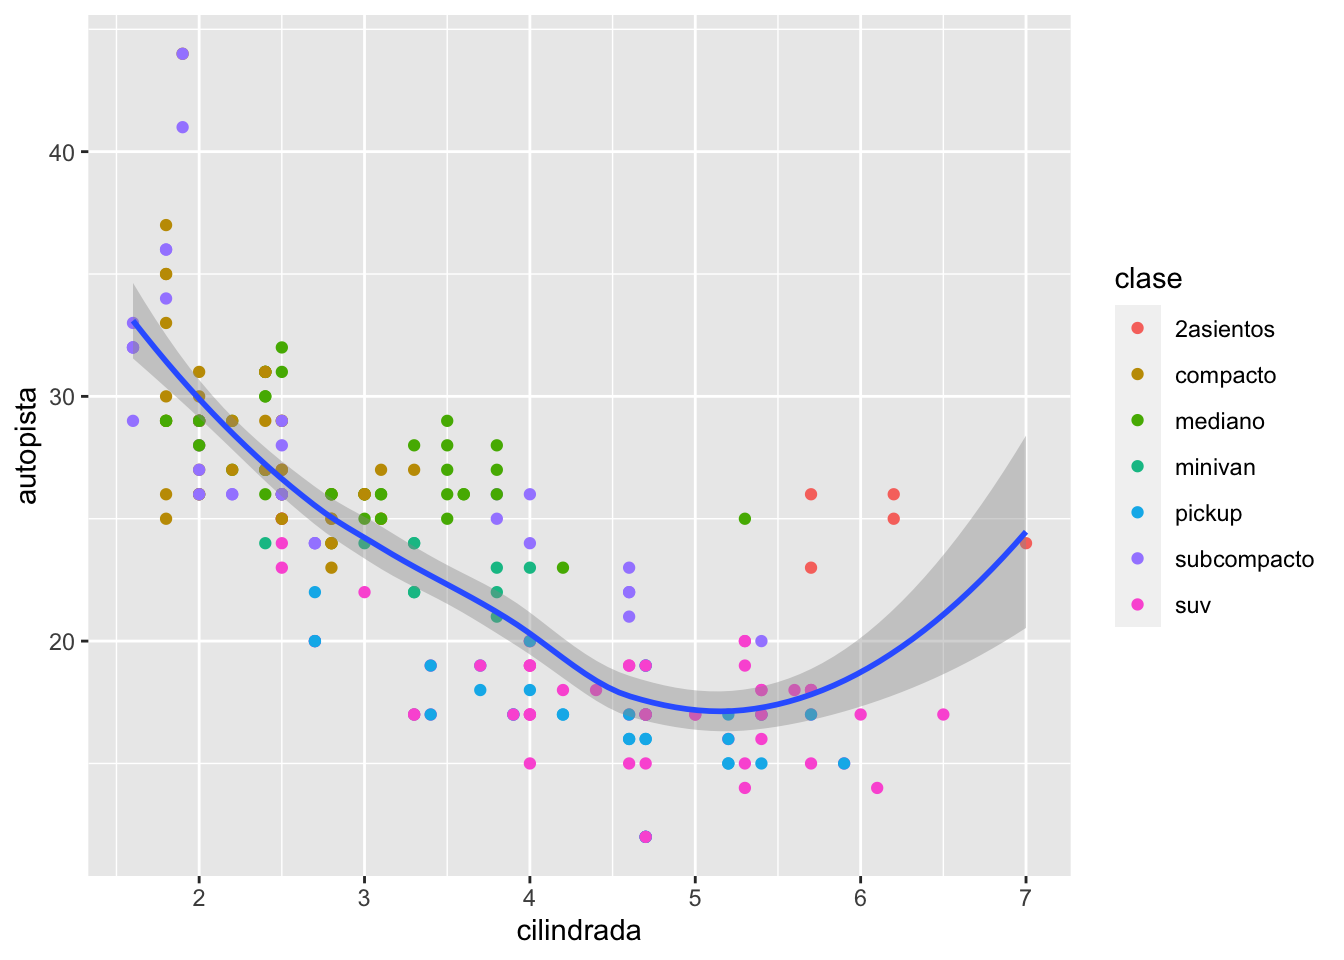
\includegraphics{Dinamica_poblacional_files/figure-latex/unnamed-chunk-40-1.pdf}

\begin{Shaded}
\begin{Highlighting}[]
\FunctionTok{summary}\NormalTok{(lambda\_terr)}
\end{Highlighting}
\end{Shaded}

\begin{verbatim}
##    Min. 1st Qu.  Median    Mean 3rd Qu.    Max. 
##  0.4089  0.9349  1.0000  1.0053  1.0538  1.7760
\end{verbatim}

\begin{Shaded}
\begin{Highlighting}[]
\FunctionTok{hist}\NormalTok{(lambda\_terr, }\AttributeTok{main =} \StringTok{"Lambda values"}\NormalTok{)}
\end{Highlighting}
\end{Shaded}

\includegraphics{Dinamica_poblacional_files/figure-latex/unnamed-chunk-40-2.pdf}

\begin{Shaded}
\begin{Highlighting}[]
\NormalTok{df\_Lamb\_epi}\OtherTok{=}\FunctionTok{as.data.frame}\NormalTok{(lambda\_epi)}
\NormalTok{df\_Lamb\_epi}\OtherTok{=}\NormalTok{df\_Lamb\_epi }\SpecialCharTok{\%\textgreater{}\%} 
  \FunctionTok{add\_column}\NormalTok{(}\AttributeTok{Habit\_Type =} \StringTok{"Epiphyte"}\NormalTok{) }\SpecialCharTok{\%\textgreater{}\%} 
  \FunctionTok{rename}\NormalTok{(}\AttributeTok{lambda=}\NormalTok{lambda\_epi)}


\NormalTok{df\_Lamb\_terr}\OtherTok{=}\FunctionTok{as.data.frame}\NormalTok{(lambda\_terr)}
\NormalTok{df\_Lamb\_terr}\OtherTok{=}\NormalTok{df\_Lamb\_terr }\SpecialCharTok{\%\textgreater{}\%} 
  \FunctionTok{add\_column}\NormalTok{(}\AttributeTok{Habit\_Type =} \StringTok{"Terrestrial"}\NormalTok{)}\SpecialCharTok{\%\textgreater{}\%} 
  \FunctionTok{rename}\NormalTok{(}\AttributeTok{lambda=}\NormalTok{lambda\_terr)}


\NormalTok{ALL\_Lambdas}\OtherTok{=}\FunctionTok{rbind}\NormalTok{(df\_Lamb\_epi, df\_Lamb\_terr)}
\end{Highlighting}
\end{Shaded}

\begin{Shaded}
\begin{Highlighting}[]
\FunctionTok{ggplot}\NormalTok{(ALL\_Lambdas, }\FunctionTok{aes}\NormalTok{(lambda, }\AttributeTok{fill=}\NormalTok{Habit\_Type ))}\SpecialCharTok{+}
  \FunctionTok{geom\_histogram}\NormalTok{(}\AttributeTok{colour=}\StringTok{"white"}\NormalTok{) }\SpecialCharTok{+} 
  \FunctionTok{facet\_wrap}\NormalTok{( }\SpecialCharTok{\textasciitilde{}}\NormalTok{Habit\_Type)}
\end{Highlighting}
\end{Shaded}

\begin{verbatim}
## `stat_bin()` using `bins = 30`. Pick better value with `binwidth`.
\end{verbatim}

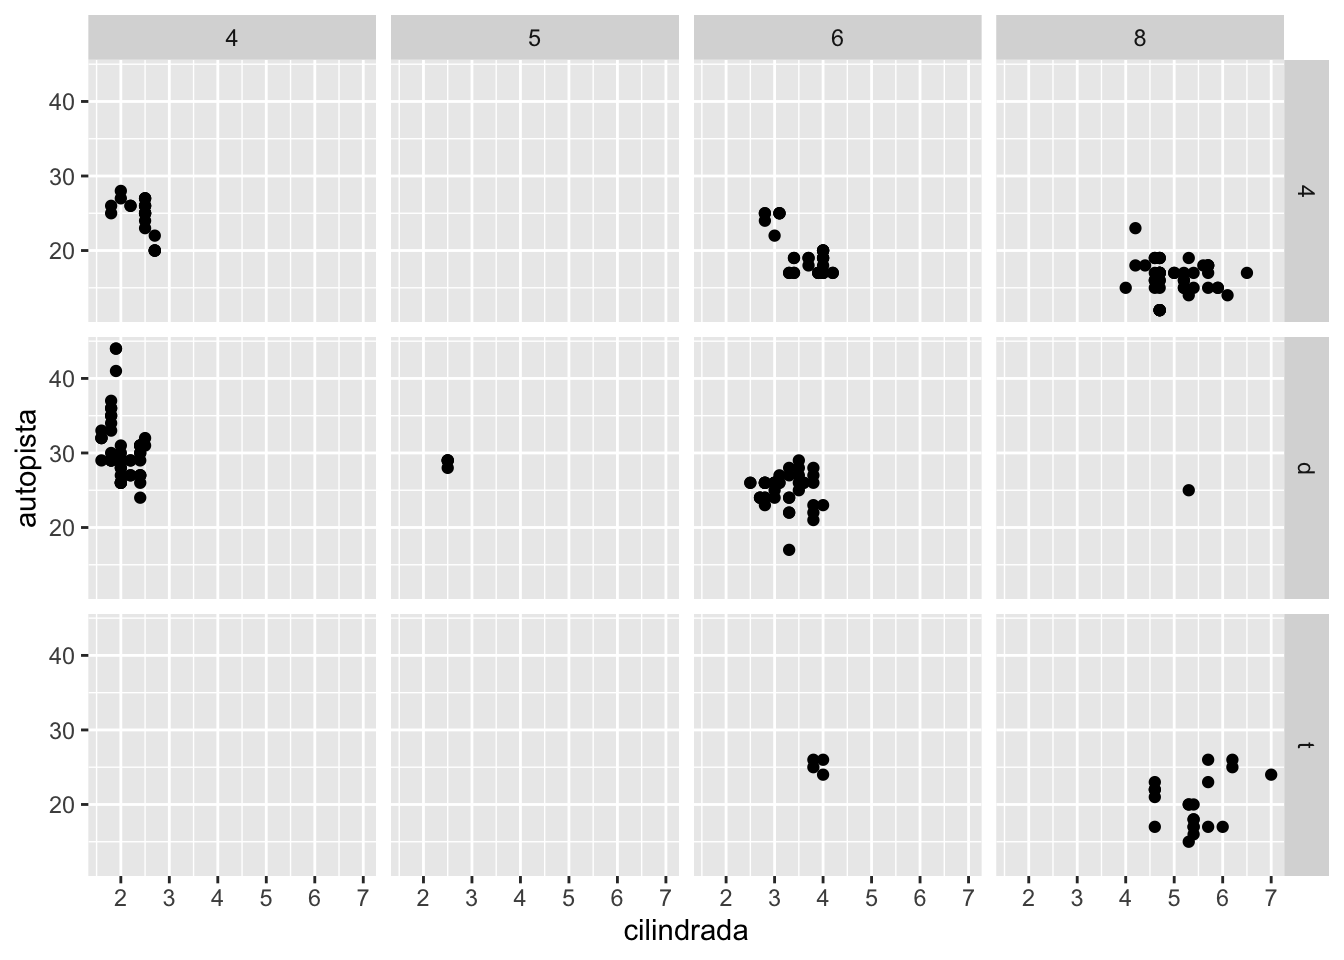
\includegraphics{Dinamica_poblacional_files/figure-latex/unnamed-chunk-42-1.pdf}

The number of populations

\begin{Shaded}
\begin{Highlighting}[]
\NormalTok{x2 }\SpecialCharTok{\%\textgreater{}\%} 
  \FunctionTok{group\_by}\NormalTok{(SpeciesAccepted) }\SpecialCharTok{\%\textgreater{}\%} 
  \FunctionTok{summarize}\NormalTok{(}\AttributeTok{n\_populations =} \FunctionTok{length}\NormalTok{(}\FunctionTok{unique}\NormalTok{(MatrixPopulation))) }\SpecialCharTok{\%\textgreater{}\%} 
  \FunctionTok{arrange}\NormalTok{(}\FunctionTok{desc}\NormalTok{(n\_populations))}
\end{Highlighting}
\end{Shaded}

\begin{verbatim}
## # A tibble: 45 x 2
##    SpeciesAccepted          n_populations
##    <chr>                            <int>
##  1 Lepanthes rubripetala               20
##  2 Lepanthes rupestris                 14
##  3 Lepanthes caritensis                13
##  4 Cypripedium calceolus                9
##  5 Orchis purpurea                      7
##  6 Neotinea ustulata                    6
##  7 Serapias cordigera                   6
##  8 Cypripedium fasciculatum             4
##  9 Epipactis atrorubens                 4
## 10 Oeceoclades maculata                 4
## # i 35 more rows
\end{verbatim}

\begin{Shaded}
\begin{Highlighting}[]
\NormalTok{compadre\_replicated\_pops }\OtherTok{\textless{}{-}}\NormalTok{ x2 }\SpecialCharTok{\%\textgreater{}\%} 
  \FunctionTok{group\_by}\NormalTok{(SpeciesAccepted) }\SpecialCharTok{\%\textgreater{}\%} 
  \FunctionTok{mutate}\NormalTok{(}\AttributeTok{n\_pops =} \FunctionTok{length}\NormalTok{(}\FunctionTok{unique}\NormalTok{(MatrixPopulation))) }\SpecialCharTok{\%\textgreater{}\%} 
  \FunctionTok{ungroup}\NormalTok{() }\SpecialCharTok{\%\textgreater{}\%}
  \FunctionTok{subset}\NormalTok{(n\_pops }\SpecialCharTok{\textgreater{}=} \DecValTok{10}\NormalTok{)}

\NormalTok{compadre\_replicated\_pops}
\end{Highlighting}
\end{Shaded}

\begin{verbatim}
## A COM(P)ADRE database ('CompadreDB') object with 3 SPECIES and 167 MATRICES.
## 
## # A tibble: 167 x 74
##    mat        MatrixID SpeciesAuthor   SpeciesAccepted CommonName Kingdom Phylum
##    <list>        <int> <chr>           <chr>           <chr>      <chr>   <chr> 
##  1 <CompdrMt>   238838 Lepanthes_rubr~ Lepanthes rubr~ <NA>       Plantae Magno~
##  2 <CompdrMt>   239751 Lepanthes_cari~ Lepanthes cari~ <NA>       Plantae Magno~
##  3 <CompdrMt>   239752 Lepanthes_cari~ Lepanthes cari~ <NA>       Plantae Magno~
##  4 <CompdrMt>   239753 Lepanthes_cari~ Lepanthes cari~ <NA>       Plantae Magno~
##  5 <CompdrMt>   239754 Lepanthes_cari~ Lepanthes cari~ <NA>       Plantae Magno~
##  6 <CompdrMt>   239755 Lepanthes_cari~ Lepanthes cari~ <NA>       Plantae Magno~
##  7 <CompdrMt>   239756 Lepanthes_cari~ Lepanthes cari~ <NA>       Plantae Magno~
##  8 <CompdrMt>   239757 Lepanthes_cari~ Lepanthes cari~ <NA>       Plantae Magno~
##  9 <CompdrMt>   239758 Lepanthes_cari~ Lepanthes cari~ <NA>       Plantae Magno~
## 10 <CompdrMt>   239759 Lepanthes_cari~ Lepanthes cari~ <NA>       Plantae Magno~
## # i 157 more rows
## # i 67 more variables: Class <chr>, Order <chr>, Family <chr>, Genus <chr>,
## #   Species <chr>, Infraspecies <chr>, InfraspeciesType <chr>,
## #   OrganismType <chr>, DicotMonoc <chr>, AngioGymno <chr>, Authors <chr>,
## #   Journal <chr>, SourceType <chr>, OtherType <chr>, YearPublication <chr>,
## #   DOI_ISBN <chr>, AdditionalSource <chr>, StudyDuration <dbl>,
## #   StudyStart <chr>, StudyEnd <chr>, ProjectionInterval <chr>, ...
\end{verbatim}

\begin{Shaded}
\begin{Highlighting}[]
\NormalTok{ggplot2}\SpecialCharTok{::}\FunctionTok{ggplot}\NormalTok{(x2, }\FunctionTok{aes}\NormalTok{(Lon, Lat)) }\SpecialCharTok{+}
  \FunctionTok{borders}\NormalTok{(}\AttributeTok{database =} \StringTok{"world"}\NormalTok{, }\AttributeTok{fill =} \StringTok{"grey80"}\NormalTok{, }\AttributeTok{col =} \ConstantTok{NA}\NormalTok{) }\SpecialCharTok{+}
  \FunctionTok{geom\_point}\NormalTok{(}\AttributeTok{col =} \StringTok{"steelblue"}\NormalTok{, }\AttributeTok{size =} \FloatTok{1.8}\NormalTok{, }\AttributeTok{alpha =} \FloatTok{0.8}\NormalTok{)}
\end{Highlighting}
\end{Shaded}

\begin{verbatim}
## Warning: Removed 28 rows containing missing values (`geom_point()`).
\end{verbatim}

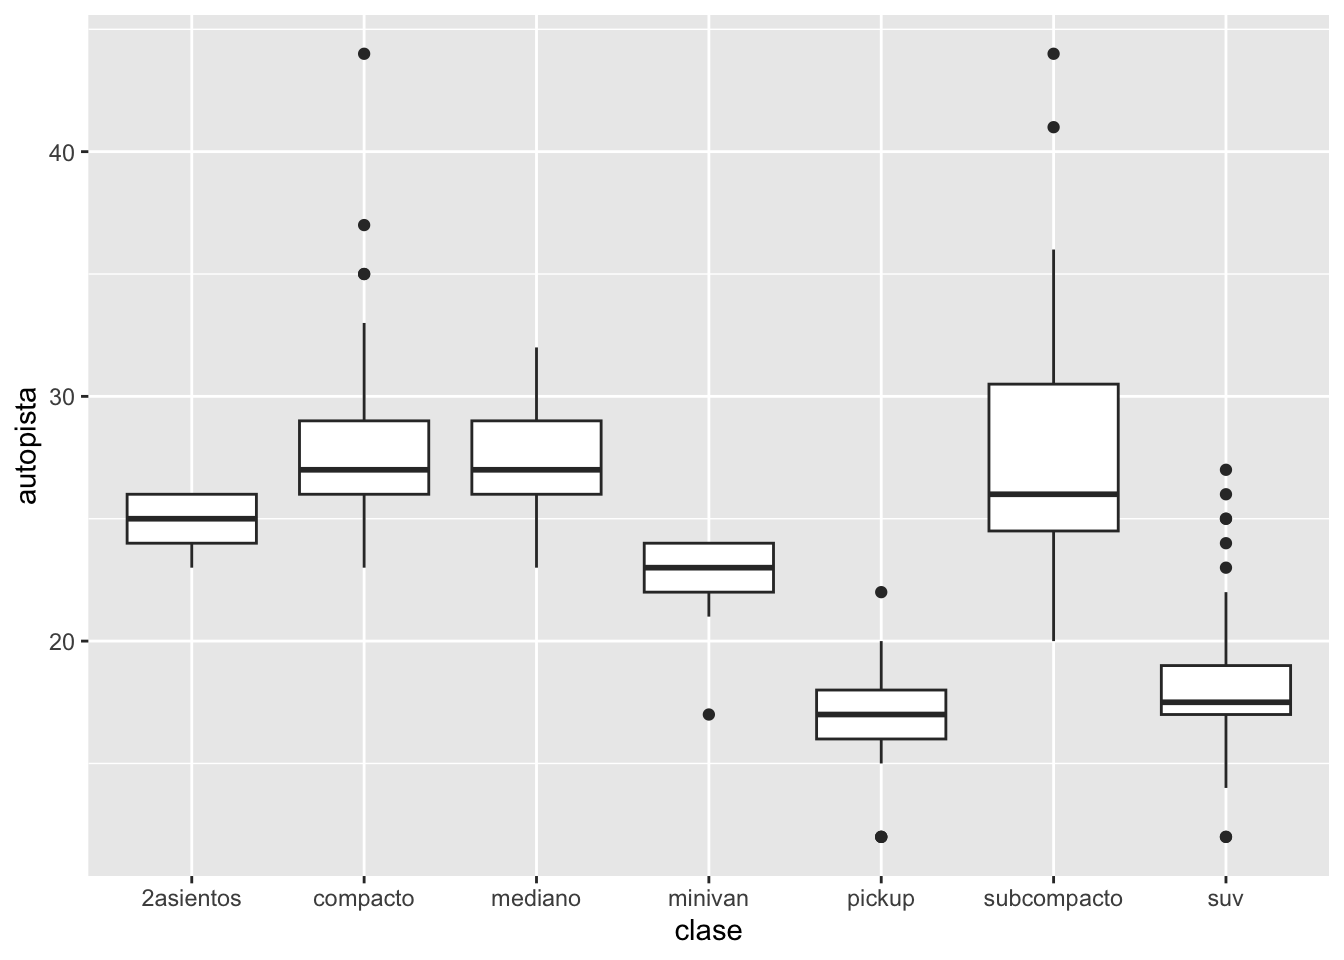
\includegraphics{Dinamica_poblacional_files/figure-latex/unnamed-chunk-45-1.pdf}

\begin{Shaded}
\begin{Highlighting}[]
\CommentTok{\# function to calculate life expectancy}
\NormalTok{lifeExpectancy }\OtherTok{\textless{}{-}} \ControlFlowTok{function}\NormalTok{(matU, startLife) \{}
\NormalTok{  N }\OtherTok{\textless{}{-}} \FunctionTok{solve}\NormalTok{(}\FunctionTok{diag}\NormalTok{(}\FunctionTok{nrow}\NormalTok{(matU)) }\SpecialCharTok{{-}}\NormalTok{ matU)}
  \FunctionTok{return}\NormalTok{(}\FunctionTok{colSums}\NormalTok{(N)[startLife])}
\NormalTok{\}}

\NormalTok{compadre\_life\_expect }\OtherTok{\textless{}{-}}\NormalTok{ x2 }\SpecialCharTok{\%\textgreater{}\%}
  \FunctionTok{filter}\NormalTok{(MatrixComposite }\SpecialCharTok{==} \StringTok{"Mean"}\NormalTok{, }\CommentTok{\# filter is the dplyr version of subset}
\NormalTok{         MatrixTreatment }\SpecialCharTok{==} \StringTok{"Unmanipulated"}\NormalTok{,}
\NormalTok{         MatrixCaptivity }\SpecialCharTok{==} \StringTok{"W"}\NormalTok{,}
         \CommentTok{\#ProjectionInterval == "1"}
\NormalTok{         ) }\SpecialCharTok{\%\textgreater{}\%} 
  \FunctionTok{mutate}\NormalTok{(}\AttributeTok{StageID =} \FunctionTok{cdb\_id\_stages}\NormalTok{(.)) }\SpecialCharTok{\%\textgreater{}\%}
  \FunctionTok{cdb\_collapse}\NormalTok{(}\AttributeTok{columns =} \StringTok{"StageID"}\NormalTok{) }\SpecialCharTok{\%\textgreater{}\%}
  \FunctionTok{cdb\_flag}\NormalTok{() }\SpecialCharTok{\%\textgreater{}\%} 
  \FunctionTok{filter}\NormalTok{(check\_NA\_U }\SpecialCharTok{==} \ConstantTok{FALSE}\NormalTok{,}
\NormalTok{         check\_zero\_U }\SpecialCharTok{==} \ConstantTok{FALSE}\NormalTok{,}
\NormalTok{         check\_singular\_U }\SpecialCharTok{==} \ConstantTok{FALSE}\NormalTok{) }\SpecialCharTok{\%\textgreater{}\%} 
  \FunctionTok{mutate}\NormalTok{(}\AttributeTok{matU =} \FunctionTok{matU}\NormalTok{(.), }\AttributeTok{start\_life =} \FunctionTok{mpm\_first\_active}\NormalTok{(.)) }\SpecialCharTok{\%\textgreater{}\%} 
  \FunctionTok{mutate}\NormalTok{(}\AttributeTok{life\_expectancy =} \FunctionTok{mapply}\NormalTok{(lifeExpectancy, matU, start\_life)) }\SpecialCharTok{\%\textgreater{}\%} 
 \CommentTok{\# filter(life\_expectancy \textgreater{}= 1) \%\textgreater{}\% }
  \FunctionTok{mutate}\NormalTok{(}\AttributeTok{OrganismType =} \FunctionTok{reorder}\NormalTok{(OrganismType, life\_expectancy, median))}
\end{Highlighting}
\end{Shaded}

\begin{verbatim}
## Warning in mpm_mean(x$mat): CompadreMat objects in given list do not all have
## the same MatrixClassOrganized. Returning MatrixClassOrganized from first list
## element
\end{verbatim}

\begin{Shaded}
\begin{Highlighting}[]
\NormalTok{ggplot2}\SpecialCharTok{::}\FunctionTok{ggplot}\NormalTok{(compadre\_life\_expect, }\FunctionTok{aes}\NormalTok{(OrganismType, life\_expectancy)) }\SpecialCharTok{+}
  \FunctionTok{geom\_boxplot}\NormalTok{() }\SpecialCharTok{+}
  \FunctionTok{scale\_y\_log10}\NormalTok{() }\SpecialCharTok{+}
  \FunctionTok{coord\_flip}\NormalTok{() }\SpecialCharTok{+}
  \FunctionTok{labs}\NormalTok{(}\AttributeTok{x =} \ConstantTok{NULL}\NormalTok{, }\AttributeTok{y =} \StringTok{"Life expectancy (years)"}\NormalTok{)}
\end{Highlighting}
\end{Shaded}

\begin{verbatim}
## Warning: Removed 1 rows containing non-finite values (`stat_boxplot()`).
\end{verbatim}

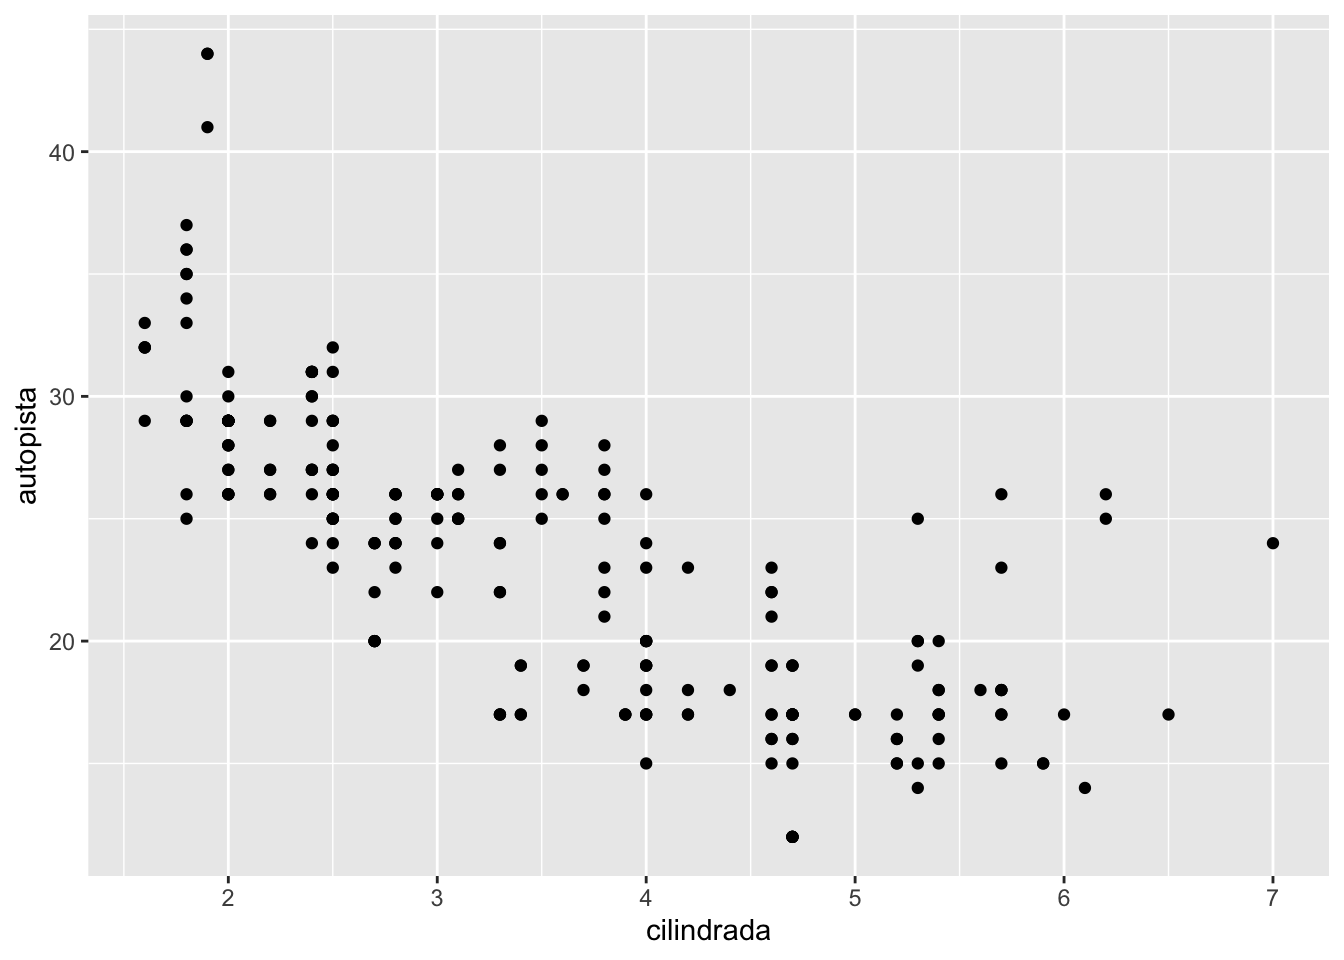
\includegraphics{Dinamica_poblacional_files/figure-latex/unnamed-chunk-46-1.pdf}

\begin{Shaded}
\begin{Highlighting}[]
\FunctionTok{library}\NormalTok{(Rcompadre)}
\FunctionTok{library}\NormalTok{(popdemo)}
\end{Highlighting}
\end{Shaded}

\begin{verbatim}
## Welcome to popdemo! This is version 1.3-0
## Use ?popdemo for an intro, or browseVignettes('popdemo') for vignettes
## Citation for popdemo is here: doi.org/10.1111/j.2041-210X.2012.00222.x
## Development and legacy versions are here: github.com/iainmstott/popdemo
\end{verbatim}

\begin{Shaded}
\begin{Highlighting}[]
\FunctionTok{data}\NormalTok{(Compadre)}


\NormalTok{Compadre}\SpecialCharTok{$}\NormalTok{matA }\OtherTok{\textless{}{-}} \FunctionTok{matA}\NormalTok{(Compadre)}

\CommentTok{\# create empty vector to store output}
\NormalTok{Compadre}\SpecialCharTok{$}\NormalTok{dim }\OtherTok{\textless{}{-}} \FunctionTok{numeric}\NormalTok{(}\FunctionTok{nrow}\NormalTok{(Compadre))}

\NormalTok{index}\SpecialCharTok{$}\NormalTok{dim }\OtherTok{\textless{}{-}} \FunctionTok{numeric}\NormalTok{(}\FunctionTok{nrow}\NormalTok{(index\_O))}
\end{Highlighting}
\end{Shaded}

\begin{verbatim}
## Warning in index$dim <- numeric(nrow(index_O)): Coercing LHS to a list
\end{verbatim}

\begin{Shaded}
\begin{Highlighting}[]
\CommentTok{\# loop through all rows of Compadre}
\ControlFlowTok{for}\NormalTok{ (i }\ControlFlowTok{in} \FunctionTok{seq\_len}\NormalTok{(}\FunctionTok{nrow}\NormalTok{(Compadre))) \{}
\NormalTok{  Compadre}\SpecialCharTok{$}\NormalTok{dim[i] }\OtherTok{\textless{}{-}} \FunctionTok{nrow}\NormalTok{(Compadre}\SpecialCharTok{$}\NormalTok{matA[[i]])}
\NormalTok{\}}

\CommentTok{\# function to determine whether matrix \textquotesingle{}mat\textquotesingle{} has any stages with no transitions}
\NormalTok{NullStages }\OtherTok{\textless{}{-}} \ControlFlowTok{function}\NormalTok{(mat) }\FunctionTok{any}\NormalTok{(}\FunctionTok{colSums}\NormalTok{(mat) }\SpecialCharTok{==} \DecValTok{0}\NormalTok{)}

\CommentTok{\# apply function to every element of A}
\NormalTok{Compadre}\SpecialCharTok{$}\NormalTok{null\_stages }\OtherTok{\textless{}{-}} \FunctionTok{sapply}\NormalTok{(Compadre}\SpecialCharTok{$}\NormalTok{matA, NullStages)}

\FunctionTok{NullStages}\NormalTok{(Compadre}\SpecialCharTok{$}\NormalTok{matA[[}\DecValTok{1}\NormalTok{]]) }\CommentTok{\# apply function to single element}
\end{Highlighting}
\end{Shaded}

\begin{verbatim}
## [1] FALSE
\end{verbatim}

\begin{Shaded}
\begin{Highlighting}[]
\NormalTok{Compadre}\SpecialCharTok{$}\NormalTok{null\_stages }\OtherTok{\textless{}{-}} \FunctionTok{sapply}\NormalTok{(}\FunctionTok{matA}\NormalTok{(Compadre), NullStages)}
\end{Highlighting}
\end{Shaded}

\hypertarget{ltre}{%
\chapter{LTRE}\label{ltre}}

Por: Adriana Ramirez Martinez

\hypertarget{introducciuxf3n-a-ltre}{%
\section{Introducción a LTRE}\label{introducciuxf3n-a-ltre}}

Ahora el primer paso es explicar a que \ldots..

\hypertarget{muxe9todos-1}{%
\section{Métodos}\label{muxe9todos-1}}

\hypertarget{metodos-de-simulaciones-1}{%
\chapter{Metodos de Simulaciones}\label{metodos-de-simulaciones-1}}

Por: ???

\hypertarget{introducciones-a-muxe9todos-de-simulaciones-1}{%
\section{Introducciones a métodos de simulaciones}\label{introducciones-a-muxe9todos-de-simulaciones-1}}

\hypertarget{ventaja-de-usar-simulaciones-1}{%
\section{Ventaja de usar simulaciones}\label{ventaja-de-usar-simulaciones-1}}

\hypertarget{ejemplo-simple-de-simulaciones-1}{%
\section{Ejemplo Simple de simulaciones}\label{ejemplo-simple-de-simulaciones-1}}

\hypertarget{el-uso-de-matrices-para-estudios-evolutivos}{%
\chapter{El uso de matrices para estudios evolutivos}\label{el-uso-de-matrices-para-estudios-evolutivos}}

Por: Roberto Salguero-Gómez

\hypertarget{section-1}{%
\section{}\label{section-1}}

\hypertarget{ppm_orquidea-sinopsis-historico}{%
\chapter{PPM\_Orquidea sinopsis historico}\label{ppm_orquidea-sinopsis-historico}}

\hypertarget{por-raymond-y-todos}{%
\section{Por: Raymond y todos}\label{por-raymond-y-todos}}

Por: Un overview de la historia de estudios PPm con orquideas

\hypertarget{compadre_orchid-ppm-y-su-uso}{%
\chapter{Compadre\_Orchid PPM y su uso}\label{compadre_orchid-ppm-y-su-uso}}

\hypertarget{raymond-y-roberto}{%
\section{Raymond y Roberto}\label{raymond-y-roberto}}

\begin{Shaded}
\begin{Highlighting}[]
\FunctionTok{library}\NormalTok{(Rcompadre)}
\FunctionTok{library}\NormalTok{(tidyverse)}
\FunctionTok{library}\NormalTok{(gt)}
\FunctionTok{library}\NormalTok{(kableExtra)}
\end{Highlighting}
\end{Shaded}

\hypertarget{load-data-from-compadre}{%
\section{\texorpdfstring{Load data from \textbf{COMPADRE}}{Load data from COMPADRE}}\label{load-data-from-compadre}}

\begin{Shaded}
\begin{Highlighting}[]
\FunctionTok{load}\NormalTok{(}\StringTok{"\textasciitilde{}/Dropbox/GitHub\_Dropbox\_Drive/GitHub/Taller\_Demo\_Peru/Taller\_Diagnostico\_Poblacional/COMPADRE\_v.6.23.5.0.RData"}\NormalTok{)}

\NormalTok{ALLSp}\OtherTok{=}\FunctionTok{as\_cdb}\NormalTok{(compadre)  }\CommentTok{\# Un baso critico: Convertir la base de datos anterior COM(P)ADRE (de clase \textquotesingle{}list\textquotesingle{}) en la base en un objeto CompadreDB.}

\FunctionTok{names}\NormalTok{(ALLSp) }\CommentTok{\# Nombre de las variables}
\end{Highlighting}
\end{Shaded}

\begin{verbatim}
##  [1] "mat"                    "MatrixID"               "SpeciesAuthor"         
##  [4] "SpeciesAccepted"        "CommonName"             "Kingdom"               
##  [7] "Phylum"                 "Class"                  "Order"                 
## [10] "Family"                 "Genus"                  "Species"               
## [13] "Infraspecies"           "InfraspeciesType"       "OrganismType"          
## [16] "DicotMonoc"             "AngioGymno"             "Authors"               
## [19] "Journal"                "SourceType"             "OtherType"             
## [22] "YearPublication"        "DOI_ISBN"               "AdditionalSource"      
## [25] "StudyDuration"          "StudyStart"             "StudyEnd"              
## [28] "ProjectionInterval"     "MatrixCriteriaSize"     "MatrixCriteriaOntogeny"
## [31] "MatrixCriteriaAge"      "MatrixPopulation"       "NumberPopulations"     
## [34] "Lat"                    "Lon"                    "Altitude"              
## [37] "Country"                "Continent"              "Ecoregion"             
## [40] "StudiedSex"             "MatrixComposite"        "MatrixSeasonal"        
## [43] "MatrixTreatment"        "MatrixCaptivity"        "MatrixStartYear"       
## [46] "MatrixStartSeason"      "MatrixStartMonth"       "MatrixEndYear"         
## [49] "MatrixEndSeason"        "MatrixEndMonth"         "CensusType"            
## [52] "MatrixSplit"            "MatrixFec"              "Observations"          
## [55] "MatrixDimension"        "SurvivalIssue"          "_Database"             
## [58] "_PopulationStatus"      "_PublicationStatus"
\end{verbatim}

\begin{Shaded}
\begin{Highlighting}[]
\NormalTok{index\_O}\OtherTok{=}\NormalTok{ALLSp }\SpecialCharTok{\%\textgreater{}\%} 
 \FunctionTok{filter}\NormalTok{(Family }\SpecialCharTok{\%in\%} \FunctionTok{c}\NormalTok{(}\StringTok{"Orchidaceae"}\NormalTok{)) }\CommentTok{\# Extraer la orquídeas de la base de datos. }
\end{Highlighting}
\end{Shaded}

\hypertarget{lista-de-especies-de-orquuxeddeas-en-la-base-de-datos-de-copadre}{%
\section{Lista de especies de orquídeas en la base de datos de COPADRE}\label{lista-de-especies-de-orquuxeddeas-en-la-base-de-datos-de-copadre}}

\begin{Shaded}
\begin{Highlighting}[]
\FunctionTok{unique}\NormalTok{(index\_O}\SpecialCharTok{$}\NormalTok{SpeciesAccepted)}
\end{Highlighting}
\end{Shaded}

\begin{verbatim}
##  [1] "Caladenia amonea"          "Caladenia argocalla"      
##  [3] "Caladenia clavigera"       "Caladenia elegans"        
##  [5] "Caladenia graniticola"     "Caladenia macroclavia"    
##  [7] "Caladenia oenochila"       "Caladenia rosella"        
##  [9] "Caladenia valida"          "Epipactis atrorubens"     
## [11] "Lepanthes rubripetala"     "Spathoglottis plicata"    
## [13] "Broughtonia cubensis"      "Cephalanthera longifolia" 
## [15] "Cleistes bifaria"          "Cypripedium calceolus"    
## [17] "Dendrophylax lindenii"     "Erycina crista-galli"     
## [19] "Lepanthes acuminata"       "Lepanthes caritensis"     
## [21] "Oncidium poikilostalix"    "Serapias cordigera"       
## [23] "Telipogon helleri"         "Aspasia principissa"      
## [25] "Guarianthe aurantiaca"     "Jacquiniella leucomelana" 
## [27] "Jacquiniella teretifolia"  "Lepanthes eltoroensis"    
## [29] "Lycaste aromatica"         "Tolumnia variegata"       
## [31] "Cleistesiopsis bifaria"    "Cleistesiopsis divaricata"
## [33] "Corallorhiza trifida"      "Cypripedium fasciculatum" 
## [35] "Cypripedium lentiginosum"  "Cypripedium parviflorum"  
## [37] "Dactylorhiza lapponica"    "Herminium monorchis"      
## [39] "Himantoglossum hircinum"   "Lepanthes rupestris"      
## [41] "Neotinea ustulata"         "Ophrys sphegodes"         
## [43] "Orchis purpurea"           "Platanthera hookeri"      
## [45] "Oeceoclades maculata"      "Brassavola cucullata"
\end{verbatim}

\hypertarget{how-many-unique-studies-1}{%
\section{How many unique studies?}\label{how-many-unique-studies-1}}

To know how long the studies were and be unique I need to select combinations of variables that make it unique.

Subset

\begin{Shaded}
\begin{Highlighting}[]
\FunctionTok{names}\NormalTok{(index\_O)}
\end{Highlighting}
\end{Shaded}

\begin{verbatim}
##  [1] "mat"                    "MatrixID"               "SpeciesAuthor"         
##  [4] "SpeciesAccepted"        "CommonName"             "Kingdom"               
##  [7] "Phylum"                 "Class"                  "Order"                 
## [10] "Family"                 "Genus"                  "Species"               
## [13] "Infraspecies"           "InfraspeciesType"       "OrganismType"          
## [16] "DicotMonoc"             "AngioGymno"             "Authors"               
## [19] "Journal"                "SourceType"             "OtherType"             
## [22] "YearPublication"        "DOI_ISBN"               "AdditionalSource"      
## [25] "StudyDuration"          "StudyStart"             "StudyEnd"              
## [28] "ProjectionInterval"     "MatrixCriteriaSize"     "MatrixCriteriaOntogeny"
## [31] "MatrixCriteriaAge"      "MatrixPopulation"       "NumberPopulations"     
## [34] "Lat"                    "Lon"                    "Altitude"              
## [37] "Country"                "Continent"              "Ecoregion"             
## [40] "StudiedSex"             "MatrixComposite"        "MatrixSeasonal"        
## [43] "MatrixTreatment"        "MatrixCaptivity"        "MatrixStartYear"       
## [46] "MatrixStartSeason"      "MatrixStartMonth"       "MatrixEndYear"         
## [49] "MatrixEndSeason"        "MatrixEndMonth"         "CensusType"            
## [52] "MatrixSplit"            "MatrixFec"              "Observations"          
## [55] "MatrixDimension"        "SurvivalIssue"          "_Database"             
## [58] "_PopulationStatus"      "_PublicationStatus"
\end{verbatim}

\begin{Shaded}
\begin{Highlighting}[]
\NormalTok{SPECIES\_O}\OtherTok{=}\NormalTok{index\_O }\SpecialCharTok{\%\textgreater{}\%} \FunctionTok{select}\NormalTok{(StudyStart, StudyEnd, SpeciesAccepted, YearPublication, Authors, DOI\_ISBN, OrganismType, MatrixPopulation,mat) }\SpecialCharTok{\%\textgreater{}\%} 
  \FunctionTok{group\_by}\NormalTok{(SpeciesAccepted, YearPublication, Authors, DOI\_ISBN, OrganismType, StudyStart, StudyEnd) }\SpecialCharTok{\%\textgreater{}\%} 
  \FunctionTok{summarize}\NormalTok{(}\AttributeTok{n\_populations =} \FunctionTok{length}\NormalTok{(}\FunctionTok{unique}\NormalTok{(MatrixPopulation))) }\SpecialCharTok{\%\textgreater{}\%} 
  \FunctionTok{arrange}\NormalTok{(}\FunctionTok{desc}\NormalTok{(n\_populations)) }\SpecialCharTok{\%\textgreater{}\%} 
  \FunctionTok{mutate}\NormalTok{(}\AttributeTok{StudyStart=}\FunctionTok{as.numeric}\NormalTok{(StudyStart)) }\SpecialCharTok{\%\textgreater{}\%} 
  \FunctionTok{mutate}\NormalTok{(}\AttributeTok{StudyEnd=}\FunctionTok{as.numeric}\NormalTok{(StudyEnd)) }\SpecialCharTok{\%\textgreater{}\%} 
  \FunctionTok{drop\_na}\NormalTok{(StudyStart, StudyEnd)}

\NormalTok{SPECIES\_O }\SpecialCharTok{\%\textgreater{}\%} \FunctionTok{kable}\NormalTok{()}
\end{Highlighting}
\end{Shaded}

\begin{tabular}{l|l|l|l|l|r|r|r}
\hline
SpeciesAccepted & YearPublication & Authors & DOI\_ISBN & OrganismType & StudyStart & StudyEnd & n\_populations\\
\hline
Lepanthes caritensis & 2018 & Crain; Tremblay; Ferguson & 10.1002/1438-390X.1002 & Epiphyte & 2010 & 2012 & 18\\
\hline
Epipactis atrorubens & 2017 & Hens; Pakanen; Jäkäläniemi; Tuomi; Kvist & 10.1016/j.biocon.2017.04.019 & Herbaceous perennial & 2000 & 2015 & 8\\
\hline
Lepanthes rubripetala & 2010 & Schödelbauerová; Tremblay; Kindlmann & 10.1007/s10531-009-9724-1 & Epiphyte & 1994 & 2007 & 8\\
\hline
Lepanthes rupestris & 2001 & Tremblay; Ackerman & 10.1006/bijl.2000.0485 & Herbaceous perennial & 1994 & 1996 & 7\\
\hline
Lepanthes rupestris & 2014 & Tremblay; McCarthy & 10.1371/journal.pone.0102859 & Herbaceous perennial & 1993 & 1996 & 7\\
\hline
Orchis purpurea & 2010 & Jacquemyns; Brys; Jongejans & 10.1890/08-2321.1 & Herbaceous perennial & 2002 & 2008 & 7\\
\hline
Lepanthes rubripetala & 2001 & Tremblay; Ackerman & 10.1006/bijl.2000.0485 & Epiphyte & 1994 & 1996 & 6\\
\hline
Lepanthes rubripetala & 2015 & Tremblay; Raventós; Ackerman; & 10.1093/aob/mcv031 & Epiphyte & 1994 & 1996 & 6\\
\hline
Neotinea ustulata & 2007 & Shefferson; Tali & 10.1111/j.1365-2745.2006.01195.x & Herbaceous perennial & 1993 & 2005 & 6\\
\hline
Serapias cordigera & 2014 & Pellegrino; Bellusci & 10.1111/boj.12204 & Herbaceous perennial & 1999 & 2012 & 6\\
\hline
Cephalanthera longifolia & 2012 & Shefferson; Kull; Tali; Kellett & 10.1890/ES11-00328.1 & Herbaceous perennial & 2002 & 2007 & 4\\
\hline
Cleistesiopsis bifaria & 1991 & Wells; Willems & 90-5103-068-1 & Herbaceous perennial & 1983 & 1990 & 4\\
\hline
Cypripedium calceolus & 2005 & Nicolè; Brzosko; Till-Bottraud & 10.1111/j.1365-2745.2005.01010.x & Herbaceous perennial & 1991 & 2000 & 4\\
\hline
Cypripedium fasciculatum & 2011 & Thorpe; Stanley; Kayne; Latham & NA & Herbaceous perennial & 1999 & 2007 & 4\\
\hline
Oeceoclades maculata & 2019 & Riverón-Giró; Raventós; Damon; García-González; Mújica & 10.1007/s10530-019-01945-7 & Herbaceous perennial & 2014 & 2016 & 4\\
\hline
Platanthera hookeri & 2007 & Reddoch; Reddoch & 10.3159/1095-5674(2007)134[369:PEOPHO]2.0.CO;2 & Herbaceous perennial & 1990 & 2005 & 4\\
\hline
Brassavola cucullata & 2020 & Ackerman; Tremblay; Pérez; Madden; Bechtold; Boeken & NA & Epiphyte & 2009 & 2014 & 3\\
\hline
Cypripedium calceolus & 2012 & Shefferson; Kull; Tali; Kellett & 10.1890/ES11-00328.1 & Herbaceous perennial & 2002 & 2007 & 3\\
\hline
Dactylorhiza lapponica & 2010 & Sletvold; Øien; Moen & 10.1016/j.biocon.2009.12.017 & Herbaceous perennial & 1990 & 2006 & 3\\
\hline
Lepanthes eltoroensis & 2001 & Tremblay; Ackerman & 10.1006/bijl.2000.0485 & Epiphyte & 1994 & 1996 & 3\\
\hline
Cleistes bifaria & 2006 & Gregg; Kéry & 10.1016/j.biocon.2005.09.044 & Herbaceous perennial & 1986 & 1996 & 2\\
\hline
Cypripedium calceolus & 2010 & García; Goñi; Guzman & 10.1111/j.1523-1739.2010.01466.x & Herbaceous perennial & 1994 & 2002 & 2\\
\hline
Erycina crista-galli & 2007 & Mondragón; Maldonado; Aguilar-Santelises & 10.1111/boj.12204 & Epiphyte & 2004 & 2005 & 2\\
\hline
Jacquiniella leucomelana & 2009 & Winkler; Hülber; Hietz & 10.1093/aob/mcp188 & Epiphyte & 2002 & 2005 & 2\\
\hline
Jacquiniella teretifolia & 2009 & Winkler; Hülber; Hietz & 10.1093/aob/mcp188 & Epiphyte & 2002 & 2005 & 2\\
\hline
Lepanthes caritensis & 1997 & Tremblay & NA & Epiphyte & 1994 & 1996 & 2\\
\hline
Lycaste aromatica & 2009 & Winkler; Hülber; Hietz & 10.1093/aob/mcp188 & Epiphyte & 2002 & 2005 & 2\\
\hline
Aspasia principissa & 2006 & Zotz; Schmidt & 10.1016/j.biocon.2005.07.022 & Epiphyte & 1997 & 2004 & 1\\
\hline
Broughtonia cubensis & 2015 & Raventós; Gonzalez; Mújica; Bonet & 10.1111/btp.12231 & Epiphyte & 2006 & 2010 & 1\\
\hline
Caladenia amonea & 2009 & Tremblay; Pérez; Larcombe; Brown; Quarmby; Bickerton; French; Bould & 10.1071/BT08167 & Epiphyte & 1996 & 2007 & 1\\
\hline
Caladenia argocalla & 2009 & Tremblay; Pérez; Larcombe; Brown; Quarmby; Bickerton; French; Bould & 10.1071/BT08167 & Epiphyte & 1996 & 2007 & 1\\
\hline
Caladenia clavigera & 2009 & Tremblay; Pérez; Larcombe; Brown; Quarmby; Bickerton; French; Bould & 10.1071/BT08167 & Epiphyte & 1996 & 2007 & 1\\
\hline
Caladenia elegans & 2009 & Tremblay; Pérez; Larcombe; Brown; Quarmby; Bickerton; French; Bould & 10.1071/BT08167 & Epiphyte & 1996 & 2007 & 1\\
\hline
Caladenia graniticola & 2009 & Tremblay; Pérez; Larcombe; Brown; Quarmby; Bickerton; French; Bould & 10.1071/BT08167 & Epiphyte & 1996 & 2007 & 1\\
\hline
Caladenia macroclavia & 2009 & Tremblay; Pérez; Larcombe; Brown; Quarmby; Bickerton; French; Bould & 10.1071/BT08167 & Epiphyte & 1996 & 2007 & 1\\
\hline
Caladenia oenochila & 2009 & Tremblay; Pérez; Larcombe; Brown; Quarmby; Bickerton; French; Bould & 10.1071/BT08167 & Epiphyte & 1996 & 2007 & 1\\
\hline
Caladenia rosella & 2009 & Tremblay; Pérez; Larcombe; Brown; Quarmby; Bickerton; French; Bould & 10.1071/BT08167 & Epiphyte & 1996 & 2007 & 1\\
\hline
Caladenia valida & 2009 & Tremblay; Pérez; Larcombe; Brown; Quarmby; Bickerton; French; Bould & 10.1071/BT08167 & Epiphyte & 1996 & 2007 & 1\\
\hline
Cleistesiopsis divaricata & 1991 & Wells; Willems & 90-5103-068-1 & Herbaceous perennial & 1983 & 1990 & 1\\
\hline
Corallorhiza trifida & 2009 & Iriondo; Giménez-Benavides; Albert; Lozano; Escudero & 978-84-8014-746-0 & Herbaceous perennial & 2001 & 2004 & 1\\
\hline
Cypripedium parviflorum & 2014 & Shefferson; Warren II; Pulliam & 10.1111/1365-2745.12281 & Herbaceous perennial & 1994 & 2012 & 1\\
\hline
Dactylorhiza lapponica & 2013 & Sletvold; Dahlgren; Øien; Moen; Ehrlén & 10.1111/gcb.12167 & Herbaceous perennial & 1981 & 2010 & 1\\
\hline
Dendrophylax lindenii & 2015 & Raventós; Gonzalez; Mújica; Bonet & 10.1111/btp.12231 & Epiphyte & 2006 & 2010 & 1\\
\hline
Epipactis atrorubens & 2011 & Jäkäläniemi; Crone; Närhi; Tuomi & 10.1890/10-1957.1 & Herbaceous perennial & 2000 & 2008 & 1\\
\hline
Guarianthe aurantiaca & 2009 & Mondragón & 10.1111/j.1442-1984.2009.00230.x & Epiphyte & 2004 & 2006 & 1\\
\hline
Herminium monorchis & 1998 & Wells; Rothery; Cox; Bamford & 10.1111/j.1095-8339.1998.tb02514.x & Herbaceous perennial & 1966 & 1995 & 1\\
\hline
Himantoglossum hircinum & 2006 & Pfeifer; Wiegand; Heinrich; Jetschke & 10.1111/j.1365-2664.2006.01148.x & Herbaceous perennial & 1976 & 2001 & 1\\
\hline
Lepanthes acuminata & 2018 & Raventós; García-González; Riverón-Giró; Damon & 10.1080/17550874.2018.1444110 & Epiphyte & 2013 & 2015 & 1\\
\hline
Oncidium poikilostalix & 2017 & García-González; Damon; Raventós; Riverón-Giró; Mújica; Solís-Montero & 10.1080/17550874.2017.1315840 & Epiphyte & 2013 & 2015 & 1\\
\hline
Oncidium poikilostalix & 2018 & Raventós; García-González; Riverón-Giró; Damon & 10.1080/17550874.2018.1444110 & Epiphyte & 2013 & 2015 & 1\\
\hline
Ophrys sphegodes & 1991 & Wells; Willems & 90-5103-068-1 & Herbaceous perennial & 1983 & 1990 & 1\\
\hline
Spathoglottis plicata & 2017 & Falcón; Ackerman; Tremblay & 10.1007/s10530-016-1318-8 & Herbaceous perennial & 2009 & 2011 & 1\\
\hline
Telipogon helleri & 2018 & Raventós; García-González; Riverón-Giró; Damon & 10.1080/17550874.2018.1444110 & Epiphyte & 2013 & 2015 & 1\\
\hline
Tolumnia variegata & 1993 & Calvo & 10.2307/1940473 & Epiphyte & 1988 & 1990 & 1\\
\hline
\end{tabular}

\begin{Shaded}
\begin{Highlighting}[]
\FunctionTok{write\_csv}\NormalTok{(SPECIES\_O, }\StringTok{"Species\_O.csv"}\NormalTok{)}
\end{Highlighting}
\end{Shaded}

\begin{Shaded}
\begin{Highlighting}[]
\NormalTok{SPECIES\_O}\SpecialCharTok{$}\NormalTok{SpeciesAccepted }\OtherTok{\textless{}{-}} \FunctionTok{fct\_reorder}\NormalTok{(SPECIES\_O}\SpecialCharTok{$}\NormalTok{SpeciesAccepted, SPECIES\_O}\SpecialCharTok{$}\NormalTok{StudyStart, }\AttributeTok{.desc =} \ConstantTok{FALSE}\NormalTok{)}

\FunctionTok{ggplot}\NormalTok{(SPECIES\_O, }\FunctionTok{aes}\NormalTok{(SpeciesAccepted, }\AttributeTok{color=}\NormalTok{OrganismType))}\SpecialCharTok{+}
  \FunctionTok{geom\_linerange}\NormalTok{(}\FunctionTok{aes}\NormalTok{(}\AttributeTok{x=}\NormalTok{ SpeciesAccepted  , }\AttributeTok{ymin=}\NormalTok{StudyStart, }\AttributeTok{ymax=}\NormalTok{StudyEnd))}\SpecialCharTok{+}
  \FunctionTok{coord\_flip}\NormalTok{()}\SpecialCharTok{+}
  \FunctionTok{theme}\NormalTok{(}\AttributeTok{legend.position =} \FunctionTok{c}\NormalTok{(}\FloatTok{0.2}\NormalTok{, }\FloatTok{0.8}\NormalTok{))}\SpecialCharTok{+}
  \FunctionTok{theme}\NormalTok{(}\AttributeTok{axis.text.x =} \FunctionTok{element\_text}\NormalTok{(}\AttributeTok{color =} \StringTok{"grey20"}\NormalTok{, }\AttributeTok{size =} \DecValTok{9}\NormalTok{, }\AttributeTok{angle =} \DecValTok{90}\NormalTok{, }\AttributeTok{hjust =}\NormalTok{ .}\DecValTok{5}\NormalTok{, }\AttributeTok{vjust =}\NormalTok{ .}\DecValTok{5}\NormalTok{, }\AttributeTok{face =} \StringTok{"plain"}\NormalTok{),}
        \AttributeTok{axis.text.y =} \FunctionTok{element\_text}\NormalTok{(}\AttributeTok{color =} \StringTok{"grey20"}\NormalTok{, }\AttributeTok{size =} \DecValTok{7}\NormalTok{, }\AttributeTok{angle =} \DecValTok{0}\NormalTok{, }\AttributeTok{hjust =} \DecValTok{1}\NormalTok{, }\AttributeTok{vjust =} \DecValTok{0}\NormalTok{, }\AttributeTok{face =} \StringTok{"plain"}\NormalTok{),  }
        \AttributeTok{axis.title.x =} \FunctionTok{element\_text}\NormalTok{(}\AttributeTok{color =} \StringTok{"grey20"}\NormalTok{, }\AttributeTok{size =} \DecValTok{12}\NormalTok{, }\AttributeTok{angle =} \DecValTok{0}\NormalTok{, }\AttributeTok{hjust =}\NormalTok{ .}\DecValTok{5}\NormalTok{, }\AttributeTok{vjust =} \DecValTok{0}\NormalTok{, }\AttributeTok{face =} \StringTok{"plain"}\NormalTok{),}
        \AttributeTok{axis.title.y =} \FunctionTok{element\_text}\NormalTok{(}\AttributeTok{color =} \StringTok{"grey20"}\NormalTok{, }\AttributeTok{size =} \DecValTok{12}\NormalTok{, }\AttributeTok{angle =} \DecValTok{90}\NormalTok{, }\AttributeTok{hjust =}\NormalTok{ .}\DecValTok{5}\NormalTok{, }\AttributeTok{vjust =}\NormalTok{ .}\DecValTok{5}\NormalTok{, }\AttributeTok{face =} \StringTok{"plain"}\NormalTok{))}\SpecialCharTok{+}
  \FunctionTok{ylab}\NormalTok{(}\StringTok{""}\NormalTok{)}\SpecialCharTok{+}
  \FunctionTok{xlab}\NormalTok{(}\StringTok{""}\NormalTok{)}
\end{Highlighting}
\end{Shaded}

\includegraphics{Dinamica_poblacional_files/figure-latex/unnamed-chunk-52-1.pdf}

\begin{Shaded}
\begin{Highlighting}[]
\NormalTok{index\_O}\OtherTok{=}\NormalTok{index\_O }\SpecialCharTok{\%\textgreater{}\%} 
  \FunctionTok{mutate}\NormalTok{(}\AttributeTok{StudyDuration=}\FunctionTok{as.numeric}\NormalTok{(StudyDuration))}

\FunctionTok{table}\NormalTok{(index\_O}\SpecialCharTok{$}\NormalTok{StudyDuration)}
\end{Highlighting}
\end{Shaded}

\begin{verbatim}
## 
##   2   3   4   5   6   7   8   9  10  11  12  13  14  16  17  19  26  30 
##   2 211  37   2  82  43  26  47  28   2   9   6  86  53   7   1   1   3
\end{verbatim}

\begin{Shaded}
\begin{Highlighting}[]
\FunctionTok{table}\NormalTok{(index\_O}\SpecialCharTok{$}\NormalTok{OrganismType)}
\end{Highlighting}
\end{Shaded}

\begin{verbatim}
## 
##             Epiphyte Herbaceous perennial 
##                  248                  399
\end{verbatim}

\begin{Shaded}
\begin{Highlighting}[]
\FunctionTok{ggplot}\NormalTok{(index\_O, }\FunctionTok{aes}\NormalTok{(StudyDuration, }\AttributeTok{fill=}\NormalTok{OrganismType))}\SpecialCharTok{+}
         \FunctionTok{geom\_histogram}\NormalTok{(}\AttributeTok{colour=}\StringTok{"white"}\NormalTok{)}\SpecialCharTok{+}
  \FunctionTok{facet\_wrap}\NormalTok{(}\SpecialCharTok{\textasciitilde{}}\NormalTok{OrganismType)}\SpecialCharTok{+}
  \FunctionTok{theme}\NormalTok{(}\AttributeTok{legend.position =} \StringTok{"none"}\NormalTok{)}
\end{Highlighting}
\end{Shaded}

\begin{verbatim}
## `stat_bin()` using `bins = 30`. Pick better value with `binwidth`.
\end{verbatim}

\begin{verbatim}
## Warning: Removed 1 rows containing non-finite values (`stat_bin()`).
\end{verbatim}

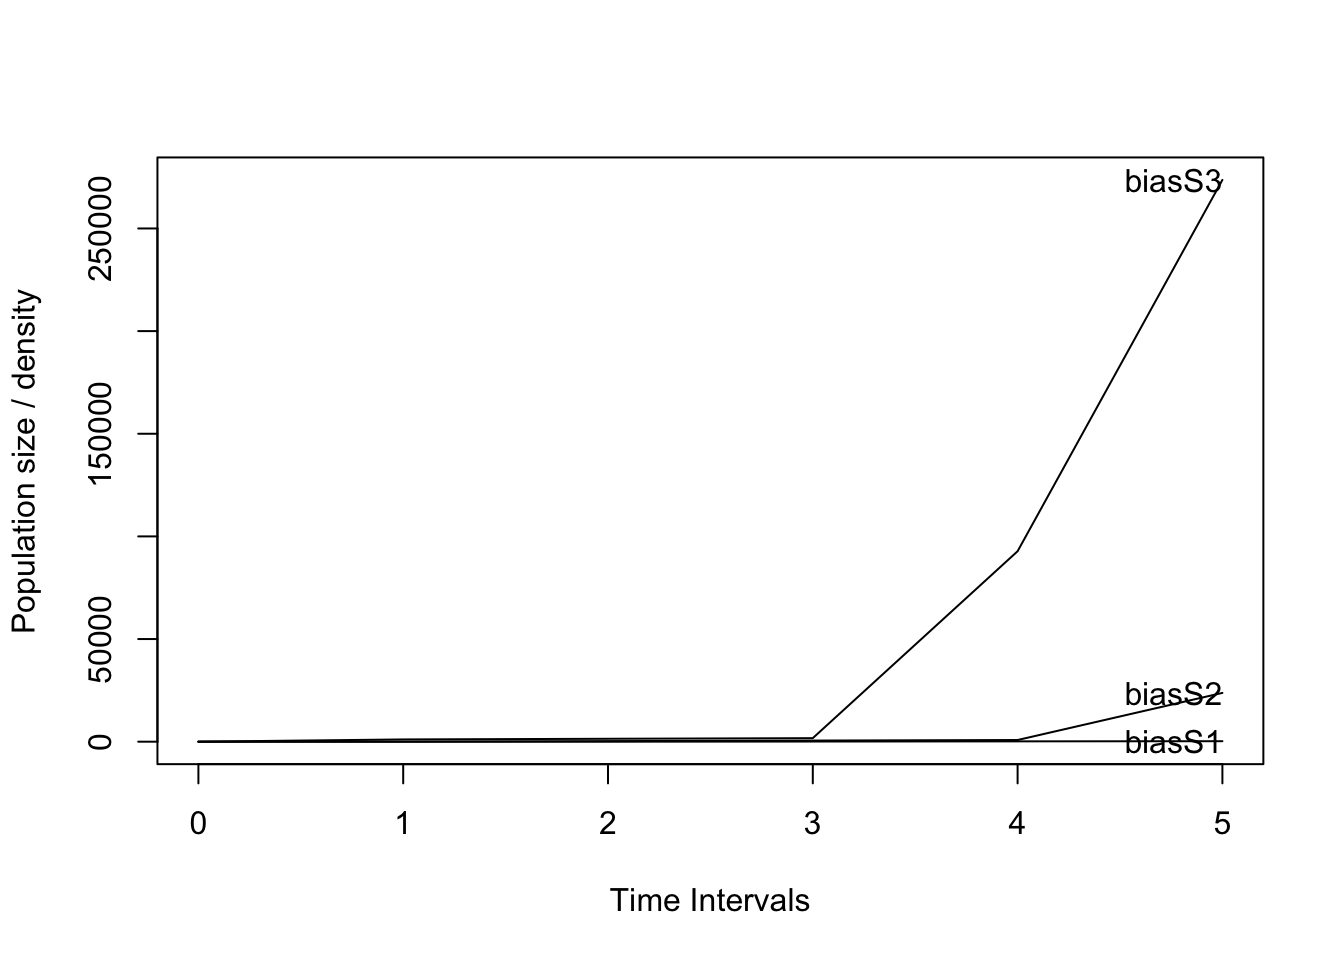
\includegraphics{Dinamica_poblacional_files/figure-latex/unnamed-chunk-53-1.pdf}

\begin{Shaded}
\begin{Highlighting}[]
\FunctionTok{ggsave}\NormalTok{(}\StringTok{"Duración\_Epi\_Ter.pdf"}\NormalTok{)}
\end{Highlighting}
\end{Shaded}

\begin{verbatim}
## Saving 6.5 x 4.5 in image
## `stat_bin()` using `bins = 30`. Pick better value with `binwidth`.
\end{verbatim}

\begin{verbatim}
## Warning: Removed 1 rows containing non-finite values (`stat_bin()`).
\end{verbatim}

\begin{Shaded}
\begin{Highlighting}[]
\FunctionTok{plot}\NormalTok{(index\_O}\SpecialCharTok{$}\NormalTok{Lon,index\_O}\SpecialCharTok{$}\NormalTok{Lat,}\AttributeTok{main =} \StringTok{"Location"}\NormalTok{)}
\end{Highlighting}
\end{Shaded}

\includegraphics{Dinamica_poblacional_files/figure-latex/unnamed-chunk-54-1.pdf}

Getting the whole database for orchids

\begin{Shaded}
\begin{Highlighting}[]
\NormalTok{index }\OtherTok{\textless{}{-}} \FunctionTok{which}\NormalTok{(compadre}\SpecialCharTok{$}\NormalTok{metadata}\SpecialCharTok{$}\NormalTok{Family}\SpecialCharTok{==}\StringTok{"Orchidaceae"}\NormalTok{) }
\FunctionTok{names}\NormalTok{(Compadre)}
\end{Highlighting}
\end{Shaded}

\begin{verbatim}
##  [1] "mat"                    "SpeciesAuthor"          "SpeciesAccepted"       
##  [4] "CommonName"             "Genus"                  "Family"                
##  [7] "Order"                  "Class"                  "Phylum"                
## [10] "Kingdom"                "OrganismType"           "DicotMonoc"            
## [13] "AngioGymno"             "Authors"                "Journal"               
## [16] "YearPublication"        "DOI_ISBN"               "AdditionalSource"      
## [19] "StudyDuration"          "StudyStart"             "StudyEnd"              
## [22] "ProjectionInterval"     "NumberPopulations"      "MatrixCriteriaSize"    
## [25] "MatrixCriteriaOntogeny" "MatrixCriteriaAge"      "MatrixPopulation"      
## [28] "Lat"                    "Lon"                    "Altitude"              
## [31] "Country"                "Continent"              "Ecoregion"             
## [34] "StudiedSex"             "MatrixComposite"        "MatrixTreatment"       
## [37] "MatrixCaptivity"        "MatrixStartYear"        "MatrixStartSeason"     
## [40] "MatrixStartMonth"       "MatrixEndYear"          "MatrixEndSeason"       
## [43] "MatrixEndMonth"         "MatrixSplit"            "MatrixFec"             
## [46] "Observation"            "MatrixDimension"        "SurvivalIssue"         
## [49] "AnnualPeriodicity"      "matA"                   "dim"                   
## [52] "null_stages"
\end{verbatim}

\begin{Shaded}
\begin{Highlighting}[]
\FunctionTok{subset}\NormalTok{(index\_O, Family }\SpecialCharTok{==}\StringTok{"Orchidaceae"}  \SpecialCharTok{\&}
\NormalTok{             MatrixDimension }\SpecialCharTok{\textgreater{}}\DecValTok{2}\NormalTok{)}
\end{Highlighting}
\end{Shaded}

\begin{verbatim}
## A COM(P)ADRE database ('CompadreDB') object with 46 SPECIES and 647 MATRICES.
## 
## # A tibble: 647 x 59
##    mat        MatrixID SpeciesAuthor   SpeciesAccepted CommonName Kingdom Phylum
##    <list>        <int> <chr>           <chr>           <chr>      <chr>   <chr> 
##  1 <CompdrMt>   238285 Caladenia_amon~ Caladenia amon~ <NA>       Plantae Trach~
##  2 <CompdrMt>   238286 Caladenia_argo~ Caladenia argo~ <NA>       Plantae Trach~
##  3 <CompdrMt>   238287 Caladenia_clav~ Caladenia clav~ <NA>       Plantae Trach~
##  4 <CompdrMt>   238288 Caladenia_eleg~ Caladenia eleg~ <NA>       Plantae Trach~
##  5 <CompdrMt>   238289 Caladenia_gran~ Caladenia gran~ <NA>       Plantae Trach~
##  6 <CompdrMt>   238290 Caladenia_macr~ Caladenia macr~ <NA>       Plantae Trach~
##  7 <CompdrMt>   238291 Caladenia_oeno~ Caladenia oeno~ <NA>       Plantae Trach~
##  8 <CompdrMt>   238292 Caladenia_rose~ Caladenia rose~ <NA>       Plantae Trach~
##  9 <CompdrMt>   238293 Caladenia_vali~ Caladenia vali~ <NA>       Plantae Trach~
## 10 <CompdrMt>   238565 Epipactis_atro~ Epipactis atro~ Darkred h~ Plantae Trach~
## # i 637 more rows
## # i 52 more variables: Class <chr>, Order <chr>, Family <chr>, Genus <chr>,
## #   Species <chr>, Infraspecies <chr>, InfraspeciesType <chr>,
## #   OrganismType <chr>, DicotMonoc <chr>, AngioGymno <chr>, Authors <chr>,
## #   Journal <chr>, SourceType <chr>, OtherType <chr>, YearPublication <chr>,
## #   DOI_ISBN <chr>, AdditionalSource <chr>, StudyDuration <dbl>,
## #   StudyStart <chr>, StudyEnd <chr>, ProjectionInterval <chr>, ...
\end{verbatim}

\begin{Shaded}
\begin{Highlighting}[]
\FunctionTok{subset}\NormalTok{(index\_O,DicotMonoc }\SpecialCharTok{==} \StringTok{"Eudicot"} \SpecialCharTok{\&} 
\NormalTok{              Country }\SpecialCharTok{\%in\%} \FunctionTok{c}\NormalTok{(}\StringTok{"USA"}\NormalTok{, }\StringTok{"CAN"}\NormalTok{) }\SpecialCharTok{\&} 
\NormalTok{              MatrixDimension }\SpecialCharTok{\textgreater{}} \DecValTok{2}\NormalTok{)}
\end{Highlighting}
\end{Shaded}

\begin{verbatim}
## A COM(P)ADRE database ('CompadreDB') object with 0 SPECIES and 0 MATRICES.
## 
## # A tibble: 0 x 59
## # i 59 variables: mat <list>, MatrixID <int>, SpeciesAuthor <chr>,
## #   SpeciesAccepted <chr>, CommonName <chr>, Kingdom <chr>, Phylum <chr>,
## #   Class <chr>, Order <chr>, Family <chr>, Genus <chr>, Species <chr>,
## #   Infraspecies <chr>, InfraspeciesType <chr>, OrganismType <chr>,
## #   DicotMonoc <chr>, AngioGymno <chr>, Authors <chr>, Journal <chr>,
## #   SourceType <chr>, OtherType <chr>, YearPublication <chr>, DOI_ISBN <chr>,
## #   AdditionalSource <chr>, StudyDuration <dbl>, StudyStart <chr>, ...
\end{verbatim}

\begin{Shaded}
\begin{Highlighting}[]
\CommentTok{\#cdb\_compare(index\_O,x)}


\NormalTok{x }\OtherTok{\textless{}{-}} \FunctionTok{subset}\NormalTok{(index\_O,Family }\SpecialCharTok{==} \StringTok{"Orchidaceae"}\NormalTok{)}

\NormalTok{x\_OT}\OtherTok{=}\NormalTok{x }\SpecialCharTok{\%\textgreater{}\%} 
  \FunctionTok{group\_by}\NormalTok{(OrganismType)}
\end{Highlighting}
\end{Shaded}

\begin{Shaded}
\begin{Highlighting}[]
\CommentTok{\#Orchids\_New=as\_cdb(index)}
\CommentTok{\#compadre$mat[index]}

\NormalTok{Compadre\_flagged }\OtherTok{\textless{}{-}} \FunctionTok{cdb\_flag}\NormalTok{(index\_O)}

\NormalTok{x }\OtherTok{\textless{}{-}} \FunctionTok{subset}\NormalTok{(Compadre\_flagged, check\_NA\_A }\SpecialCharTok{==} \ConstantTok{FALSE} \SpecialCharTok{\&}\NormalTok{ check\_ergodic }\SpecialCharTok{==} \ConstantTok{TRUE}\NormalTok{)}

\NormalTok{lambdaVals }\OtherTok{\textless{}{-}} \FunctionTok{sapply}\NormalTok{(}\FunctionTok{matA}\NormalTok{(x), popdemo}\SpecialCharTok{::}\NormalTok{eigs, }\AttributeTok{what=}\StringTok{"lambda"}\NormalTok{)}
\FunctionTok{summary}\NormalTok{(lambdaVals)}
\end{Highlighting}
\end{Shaded}

\begin{verbatim}
##    Min. 1st Qu.  Median    Mean 3rd Qu.    Max. 
##  0.3888  0.9635  0.9973  0.9944  1.0232  1.7760
\end{verbatim}

\begin{Shaded}
\begin{Highlighting}[]
\FunctionTok{hist}\NormalTok{(lambdaVals, }\AttributeTok{main =} \StringTok{"Lambda values"}\NormalTok{)}
\end{Highlighting}
\end{Shaded}

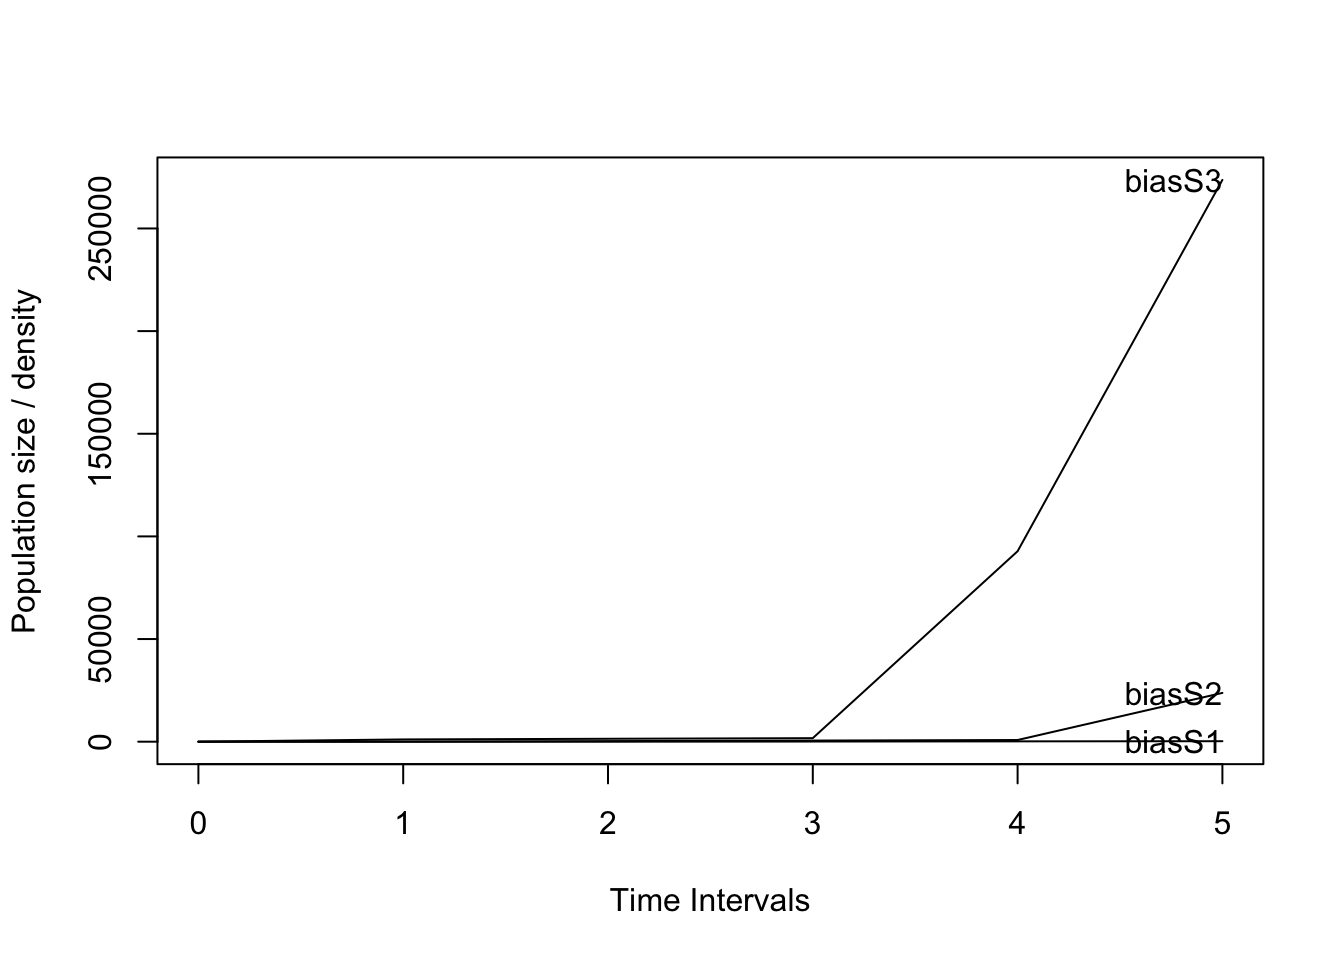
\includegraphics{Dinamica_poblacional_files/figure-latex/unnamed-chunk-56-1.pdf}

\begin{Shaded}
\begin{Highlighting}[]
\FunctionTok{library}\NormalTok{(purrr)}
\NormalTok{lambdaVals1 }\OtherTok{\textless{}{-}} \FunctionTok{map\_dbl}\NormalTok{(}\FunctionTok{matA}\NormalTok{(x), }\SpecialCharTok{\textasciitilde{}}\NormalTok{popdemo}\SpecialCharTok{::}\FunctionTok{eigs}\NormalTok{(.x, }\AttributeTok{what=}\StringTok{"lambda"}\NormalTok{))}
 
 
\CommentTok{\#Or with popbio, which avoids some warning messages…}
\NormalTok{lambdaVals2 }\OtherTok{\textless{}{-}} \FunctionTok{map\_dbl}\NormalTok{(}\FunctionTok{matA}\NormalTok{(x), }\SpecialCharTok{\textasciitilde{}}\NormalTok{popbio}\SpecialCharTok{::}\FunctionTok{lambda}\NormalTok{(.x))}
\end{Highlighting}
\end{Shaded}

\begin{Shaded}
\begin{Highlighting}[]
\NormalTok{x2}\OtherTok{=}\NormalTok{x }\SpecialCharTok{\%\textgreater{}\%} 
  \FunctionTok{mutate}\NormalTok{(}\AttributeTok{OrganismType =} \FunctionTok{case\_when}\NormalTok{(}
\NormalTok{    Genus }\SpecialCharTok{==}  \StringTok{"Caladenia"} \SpecialCharTok{\&}\NormalTok{ OrganismType }\SpecialCharTok{==} \StringTok{"Epiphyte"} \SpecialCharTok{\textasciitilde{}} \StringTok{"Herbaceous perennial"}\NormalTok{,}
    \ConstantTok{TRUE} \SpecialCharTok{\textasciitilde{}}\NormalTok{ OrganismType}
\NormalTok{  ))}

\NormalTok{epi}\OtherTok{=}\NormalTok{x2 }\SpecialCharTok{\%\textgreater{}\%} 
  \FunctionTok{filter}\NormalTok{(OrganismType}\SpecialCharTok{==}\StringTok{"Epiphyte"}\NormalTok{)}

\NormalTok{terr}\OtherTok{=}\NormalTok{x2 }\SpecialCharTok{\%\textgreater{}\%} 
  \FunctionTok{filter}\NormalTok{(OrganismType}\SpecialCharTok{==}\StringTok{"Herbaceous perennial"}\NormalTok{)}
\end{Highlighting}
\end{Shaded}

Compadre\_flagged \textless- cdb\_flag(index\_O)

x \textless- subset(Compadre\_flagged, check\_NA\_A == FALSE \& check\_ergodic == TRUE)

lambdaVals \textless- sapply(matA(x), popdemo::eigs, what=``lambda'')
summary(lambdaVals)
hist(lambdaVals, main = ``Lambda values'')

\begin{Shaded}
\begin{Highlighting}[]
\NormalTok{Compadre\_flagged\_epi }\OtherTok{\textless{}{-}} \FunctionTok{cdb\_flag}\NormalTok{(epi)}

\NormalTok{x\_epi }\OtherTok{\textless{}{-}} \FunctionTok{subset}\NormalTok{(Compadre\_flagged\_epi, check\_NA\_A }\SpecialCharTok{==} \ConstantTok{FALSE} \SpecialCharTok{\&}\NormalTok{ check\_ergodic }\SpecialCharTok{==} \ConstantTok{TRUE}\NormalTok{)}

\CommentTok{\#sapply(matA(x\_epi), popdemo::eigs, what="lambda")}

\FunctionTok{library}\NormalTok{(purrr)}
\NormalTok{lambda\_epi }\OtherTok{\textless{}{-}} \FunctionTok{map\_dbl}\NormalTok{(}\FunctionTok{matA}\NormalTok{(x\_epi), }\SpecialCharTok{\textasciitilde{}}\NormalTok{popdemo}\SpecialCharTok{::}\FunctionTok{eigs}\NormalTok{(.x, }\AttributeTok{what=}\StringTok{"lambda"}\NormalTok{))}

\CommentTok{\#Or with popbio, which avoids some warning messages…}
\NormalTok{lambda\_terr }\OtherTok{\textless{}{-}} \FunctionTok{map\_dbl}\NormalTok{(}\FunctionTok{matA}\NormalTok{(terr), }\SpecialCharTok{\textasciitilde{}}\NormalTok{popbio}\SpecialCharTok{::}\FunctionTok{lambda}\NormalTok{(.x))}
\end{Highlighting}
\end{Shaded}

\begin{Shaded}
\begin{Highlighting}[]
\FunctionTok{summary}\NormalTok{(lambda\_epi)}
\end{Highlighting}
\end{Shaded}

\begin{verbatim}
##    Min. 1st Qu.  Median    Mean 3rd Qu.    Max. 
##  0.3888  0.9874  0.9972  0.9784  1.0027  1.3592
\end{verbatim}

\begin{Shaded}
\begin{Highlighting}[]
\FunctionTok{hist}\NormalTok{(lambda\_epi, }\AttributeTok{main =} \StringTok{"Lambda values"}\NormalTok{)}
\end{Highlighting}
\end{Shaded}

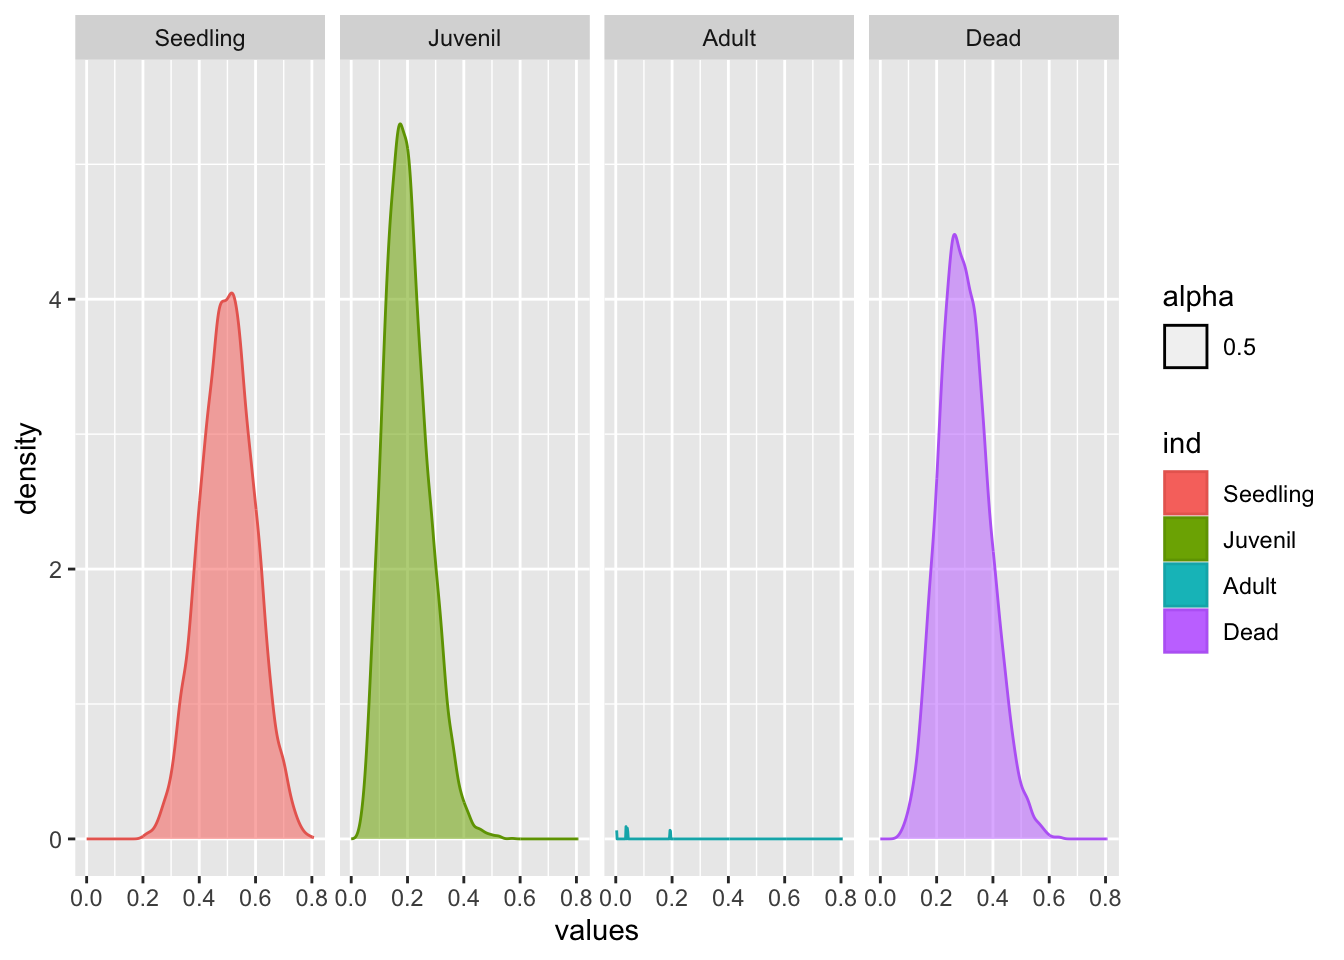
\includegraphics{Dinamica_poblacional_files/figure-latex/unnamed-chunk-60-1.pdf}

\begin{Shaded}
\begin{Highlighting}[]
\FunctionTok{summary}\NormalTok{(lambda\_terr)}
\end{Highlighting}
\end{Shaded}

\begin{verbatim}
##    Min. 1st Qu.  Median    Mean 3rd Qu.    Max. 
##  0.4089  0.9349  1.0000  1.0053  1.0538  1.7760
\end{verbatim}

\begin{Shaded}
\begin{Highlighting}[]
\FunctionTok{hist}\NormalTok{(lambda\_terr, }\AttributeTok{main =} \StringTok{"Lambda values"}\NormalTok{)}
\end{Highlighting}
\end{Shaded}

\includegraphics{Dinamica_poblacional_files/figure-latex/unnamed-chunk-60-2.pdf}

\begin{Shaded}
\begin{Highlighting}[]
\NormalTok{df\_Lamb\_epi}\OtherTok{=}\FunctionTok{as.data.frame}\NormalTok{(lambda\_epi)}
\NormalTok{df\_Lamb\_epi}\OtherTok{=}\NormalTok{df\_Lamb\_epi }\SpecialCharTok{\%\textgreater{}\%} 
  \FunctionTok{add\_column}\NormalTok{(}\AttributeTok{Habit\_Type =} \StringTok{"Epiphyte"}\NormalTok{) }\SpecialCharTok{\%\textgreater{}\%} 
  \FunctionTok{rename}\NormalTok{(}\AttributeTok{lambda=}\NormalTok{lambda\_epi)}


\NormalTok{df\_Lamb\_terr}\OtherTok{=}\FunctionTok{as.data.frame}\NormalTok{(lambda\_terr)}
\NormalTok{df\_Lamb\_terr}\OtherTok{=}\NormalTok{df\_Lamb\_terr }\SpecialCharTok{\%\textgreater{}\%} 
  \FunctionTok{add\_column}\NormalTok{(}\AttributeTok{Habit\_Type =} \StringTok{"Terrestrial"}\NormalTok{)}\SpecialCharTok{\%\textgreater{}\%} 
  \FunctionTok{rename}\NormalTok{(}\AttributeTok{lambda=}\NormalTok{lambda\_terr)}


\NormalTok{ALL\_Lambdas}\OtherTok{=}\FunctionTok{rbind}\NormalTok{(df\_Lamb\_epi, df\_Lamb\_terr)}
\end{Highlighting}
\end{Shaded}

\begin{Shaded}
\begin{Highlighting}[]
\FunctionTok{ggplot}\NormalTok{(ALL\_Lambdas, }\FunctionTok{aes}\NormalTok{(lambda, }\AttributeTok{fill=}\NormalTok{Habit\_Type ))}\SpecialCharTok{+}
  \FunctionTok{geom\_histogram}\NormalTok{(}\AttributeTok{colour=}\StringTok{"white"}\NormalTok{) }\SpecialCharTok{+} 
  \FunctionTok{facet\_wrap}\NormalTok{( }\SpecialCharTok{\textasciitilde{}}\NormalTok{Habit\_Type)}
\end{Highlighting}
\end{Shaded}

\begin{verbatim}
## `stat_bin()` using `bins = 30`. Pick better value with `binwidth`.
\end{verbatim}

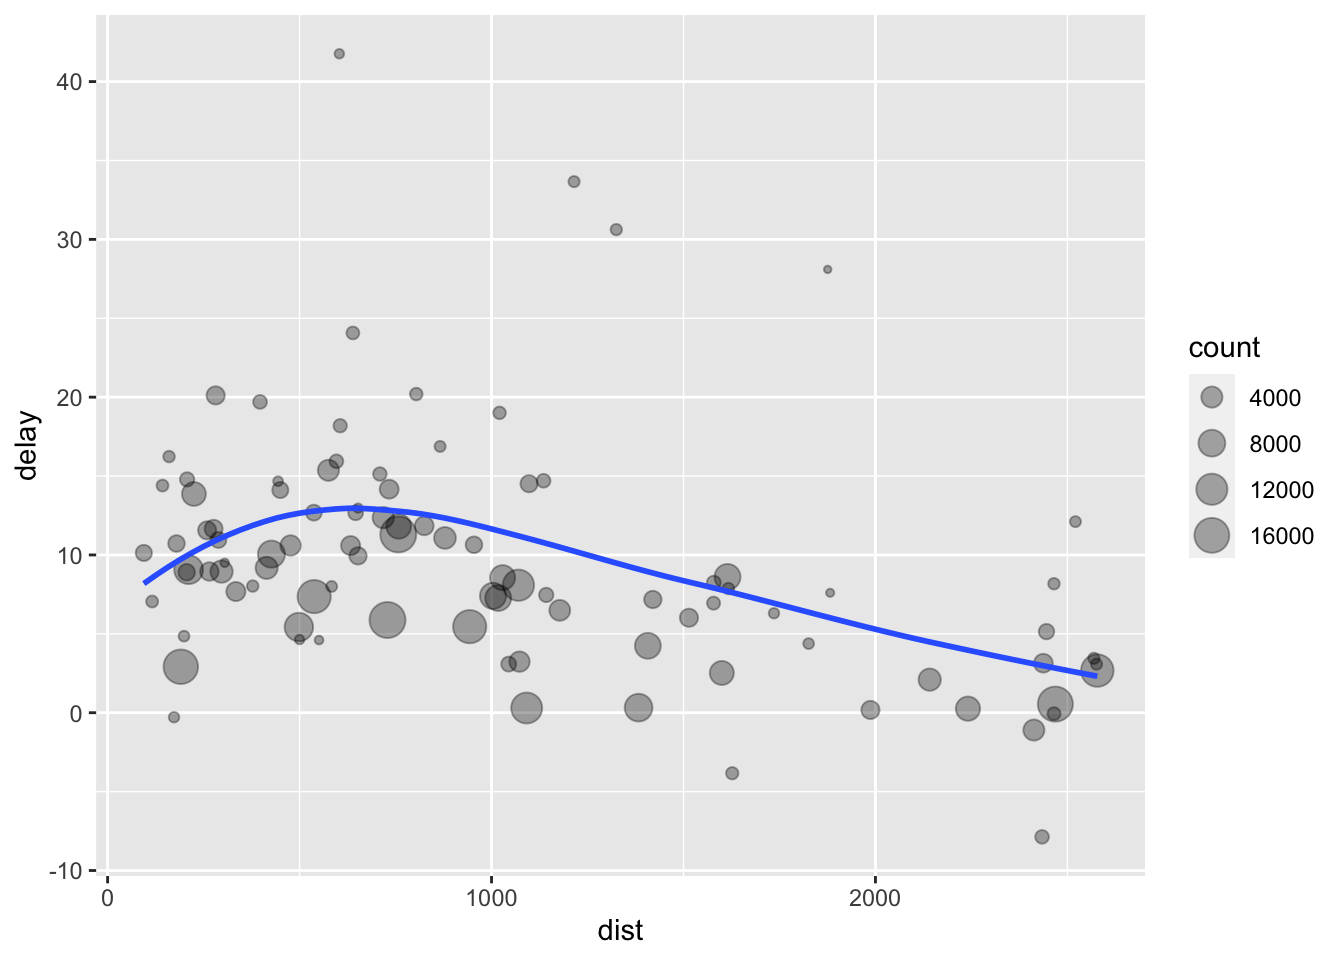
\includegraphics{Dinamica_poblacional_files/figure-latex/unnamed-chunk-62-1.pdf}

The number of populations

\begin{Shaded}
\begin{Highlighting}[]
\NormalTok{x2 }\SpecialCharTok{\%\textgreater{}\%} 
  \FunctionTok{group\_by}\NormalTok{(SpeciesAccepted) }\SpecialCharTok{\%\textgreater{}\%} 
  \FunctionTok{summarize}\NormalTok{(}\AttributeTok{n\_populations =} \FunctionTok{length}\NormalTok{(}\FunctionTok{unique}\NormalTok{(MatrixPopulation))) }\SpecialCharTok{\%\textgreater{}\%} 
  \FunctionTok{arrange}\NormalTok{(}\FunctionTok{desc}\NormalTok{(n\_populations))}
\end{Highlighting}
\end{Shaded}

\begin{verbatim}
## # A tibble: 45 x 2
##    SpeciesAccepted          n_populations
##    <chr>                            <int>
##  1 Lepanthes rubripetala               20
##  2 Lepanthes rupestris                 14
##  3 Lepanthes caritensis                13
##  4 Cypripedium calceolus                9
##  5 Orchis purpurea                      7
##  6 Neotinea ustulata                    6
##  7 Serapias cordigera                   6
##  8 Cypripedium fasciculatum             4
##  9 Epipactis atrorubens                 4
## 10 Oeceoclades maculata                 4
## # i 35 more rows
\end{verbatim}

\begin{Shaded}
\begin{Highlighting}[]
\NormalTok{compadre\_replicated\_pops }\OtherTok{\textless{}{-}}\NormalTok{ x2 }\SpecialCharTok{\%\textgreater{}\%} 
  \FunctionTok{group\_by}\NormalTok{(SpeciesAccepted) }\SpecialCharTok{\%\textgreater{}\%} 
  \FunctionTok{mutate}\NormalTok{(}\AttributeTok{n\_pops =} \FunctionTok{length}\NormalTok{(}\FunctionTok{unique}\NormalTok{(MatrixPopulation))) }\SpecialCharTok{\%\textgreater{}\%} 
  \FunctionTok{ungroup}\NormalTok{() }\SpecialCharTok{\%\textgreater{}\%}
  \FunctionTok{subset}\NormalTok{(n\_pops }\SpecialCharTok{\textgreater{}=} \DecValTok{10}\NormalTok{)}

\NormalTok{compadre\_replicated\_pops}
\end{Highlighting}
\end{Shaded}

\begin{verbatim}
## A COM(P)ADRE database ('CompadreDB') object with 3 SPECIES and 167 MATRICES.
## 
## # A tibble: 167 x 74
##    mat        MatrixID SpeciesAuthor   SpeciesAccepted CommonName Kingdom Phylum
##    <list>        <int> <chr>           <chr>           <chr>      <chr>   <chr> 
##  1 <CompdrMt>   238838 Lepanthes_rubr~ Lepanthes rubr~ <NA>       Plantae Magno~
##  2 <CompdrMt>   239751 Lepanthes_cari~ Lepanthes cari~ <NA>       Plantae Magno~
##  3 <CompdrMt>   239752 Lepanthes_cari~ Lepanthes cari~ <NA>       Plantae Magno~
##  4 <CompdrMt>   239753 Lepanthes_cari~ Lepanthes cari~ <NA>       Plantae Magno~
##  5 <CompdrMt>   239754 Lepanthes_cari~ Lepanthes cari~ <NA>       Plantae Magno~
##  6 <CompdrMt>   239755 Lepanthes_cari~ Lepanthes cari~ <NA>       Plantae Magno~
##  7 <CompdrMt>   239756 Lepanthes_cari~ Lepanthes cari~ <NA>       Plantae Magno~
##  8 <CompdrMt>   239757 Lepanthes_cari~ Lepanthes cari~ <NA>       Plantae Magno~
##  9 <CompdrMt>   239758 Lepanthes_cari~ Lepanthes cari~ <NA>       Plantae Magno~
## 10 <CompdrMt>   239759 Lepanthes_cari~ Lepanthes cari~ <NA>       Plantae Magno~
## # i 157 more rows
## # i 67 more variables: Class <chr>, Order <chr>, Family <chr>, Genus <chr>,
## #   Species <chr>, Infraspecies <chr>, InfraspeciesType <chr>,
## #   OrganismType <chr>, DicotMonoc <chr>, AngioGymno <chr>, Authors <chr>,
## #   Journal <chr>, SourceType <chr>, OtherType <chr>, YearPublication <chr>,
## #   DOI_ISBN <chr>, AdditionalSource <chr>, StudyDuration <dbl>,
## #   StudyStart <chr>, StudyEnd <chr>, ProjectionInterval <chr>, ...
\end{verbatim}

\begin{Shaded}
\begin{Highlighting}[]
\NormalTok{ggplot2}\SpecialCharTok{::}\FunctionTok{ggplot}\NormalTok{(x2, }\FunctionTok{aes}\NormalTok{(Lon, Lat)) }\SpecialCharTok{+}
  \FunctionTok{borders}\NormalTok{(}\AttributeTok{database =} \StringTok{"world"}\NormalTok{, }\AttributeTok{fill =} \StringTok{"grey80"}\NormalTok{, }\AttributeTok{col =} \ConstantTok{NA}\NormalTok{) }\SpecialCharTok{+}
  \FunctionTok{geom\_point}\NormalTok{(}\AttributeTok{col =} \StringTok{"steelblue"}\NormalTok{, }\AttributeTok{size =} \FloatTok{1.8}\NormalTok{, }\AttributeTok{alpha =} \FloatTok{0.8}\NormalTok{)}
\end{Highlighting}
\end{Shaded}

\begin{verbatim}
## Warning: Removed 28 rows containing missing values (`geom_point()`).
\end{verbatim}

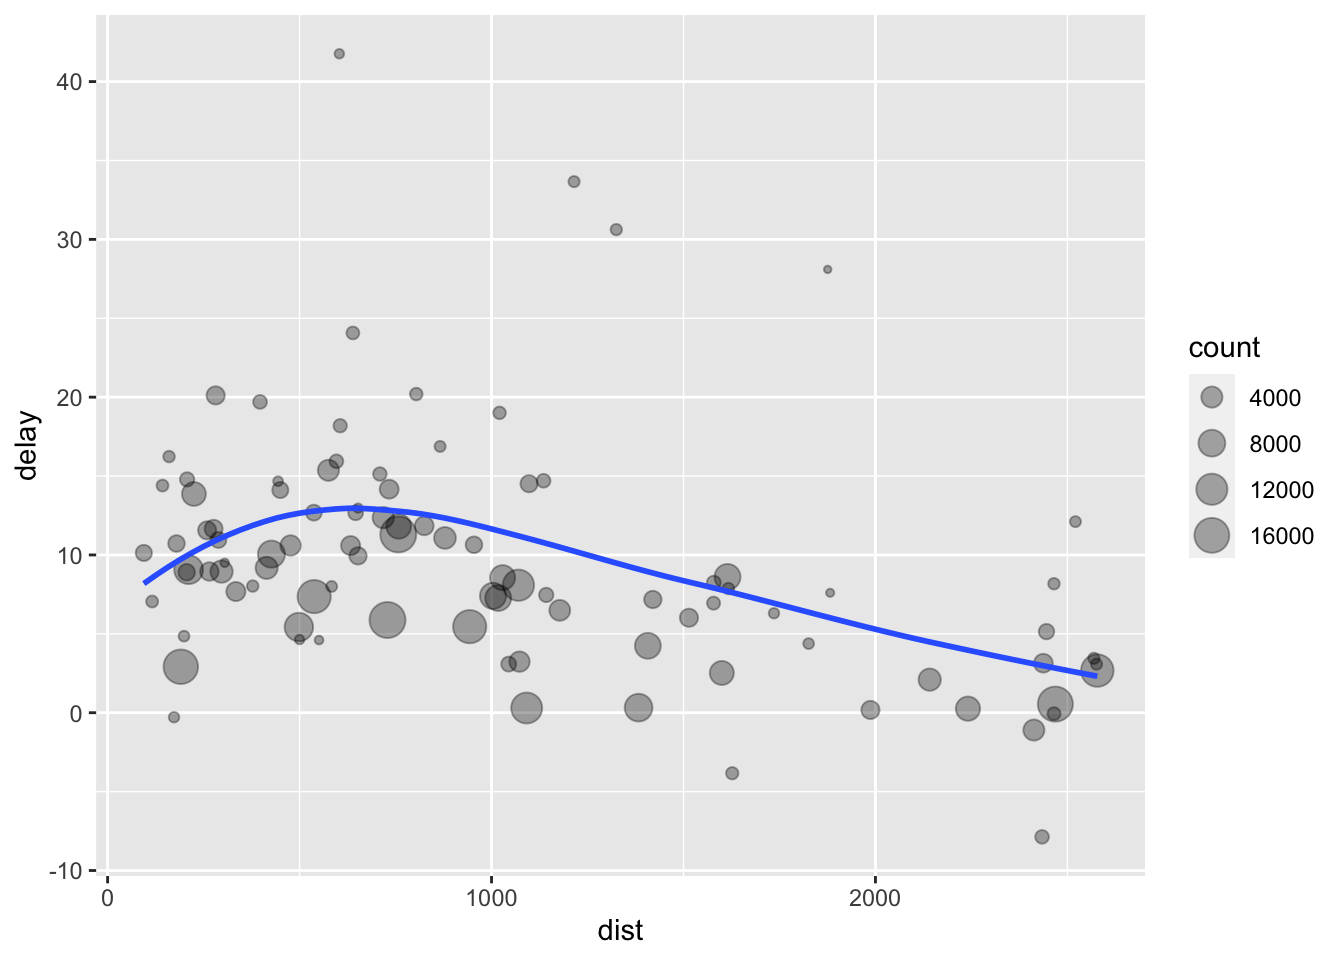
\includegraphics{Dinamica_poblacional_files/figure-latex/unnamed-chunk-65-1.pdf}

\begin{Shaded}
\begin{Highlighting}[]
\CommentTok{\# function to calculate life expectancy}
\NormalTok{lifeExpectancy }\OtherTok{\textless{}{-}} \ControlFlowTok{function}\NormalTok{(matU, startLife) \{}
\NormalTok{  N }\OtherTok{\textless{}{-}} \FunctionTok{solve}\NormalTok{(}\FunctionTok{diag}\NormalTok{(}\FunctionTok{nrow}\NormalTok{(matU)) }\SpecialCharTok{{-}}\NormalTok{ matU)}
  \FunctionTok{return}\NormalTok{(}\FunctionTok{colSums}\NormalTok{(N)[startLife])}
\NormalTok{\}}

\NormalTok{compadre\_life\_expect }\OtherTok{\textless{}{-}}\NormalTok{ x2 }\SpecialCharTok{\%\textgreater{}\%}
  \FunctionTok{filter}\NormalTok{(MatrixComposite }\SpecialCharTok{==} \StringTok{"Mean"}\NormalTok{, }\CommentTok{\# filter is the dplyr version of subset}
\NormalTok{         MatrixTreatment }\SpecialCharTok{==} \StringTok{"Unmanipulated"}\NormalTok{,}
\NormalTok{         MatrixCaptivity }\SpecialCharTok{==} \StringTok{"W"}\NormalTok{,}
         \CommentTok{\#ProjectionInterval == "1"}
\NormalTok{         ) }\SpecialCharTok{\%\textgreater{}\%} 
  \FunctionTok{mutate}\NormalTok{(}\AttributeTok{StageID =} \FunctionTok{cdb\_id\_stages}\NormalTok{(.)) }\SpecialCharTok{\%\textgreater{}\%}
  \FunctionTok{cdb\_collapse}\NormalTok{(}\AttributeTok{columns =} \StringTok{"StageID"}\NormalTok{) }\SpecialCharTok{\%\textgreater{}\%}
  \FunctionTok{cdb\_flag}\NormalTok{() }\SpecialCharTok{\%\textgreater{}\%} 
  \FunctionTok{filter}\NormalTok{(check\_NA\_U }\SpecialCharTok{==} \ConstantTok{FALSE}\NormalTok{,}
\NormalTok{         check\_zero\_U }\SpecialCharTok{==} \ConstantTok{FALSE}\NormalTok{,}
\NormalTok{         check\_singular\_U }\SpecialCharTok{==} \ConstantTok{FALSE}\NormalTok{) }\SpecialCharTok{\%\textgreater{}\%} 
  \FunctionTok{mutate}\NormalTok{(}\AttributeTok{matU =} \FunctionTok{matU}\NormalTok{(.), }\AttributeTok{start\_life =} \FunctionTok{mpm\_first\_active}\NormalTok{(.)) }\SpecialCharTok{\%\textgreater{}\%} 
  \FunctionTok{mutate}\NormalTok{(}\AttributeTok{life\_expectancy =} \FunctionTok{mapply}\NormalTok{(lifeExpectancy, matU, start\_life)) }\SpecialCharTok{\%\textgreater{}\%} 
 \CommentTok{\# filter(life\_expectancy \textgreater{}= 1) \%\textgreater{}\% }
  \FunctionTok{mutate}\NormalTok{(}\AttributeTok{OrganismType =} \FunctionTok{reorder}\NormalTok{(OrganismType, life\_expectancy, median))}
\end{Highlighting}
\end{Shaded}

\begin{verbatim}
## Warning in mpm_mean(x$mat): CompadreMat objects in given list do not all have
## the same MatrixClassOrganized. Returning MatrixClassOrganized from first list
## element
\end{verbatim}

\begin{Shaded}
\begin{Highlighting}[]
\NormalTok{ggplot2}\SpecialCharTok{::}\FunctionTok{ggplot}\NormalTok{(compadre\_life\_expect, }\FunctionTok{aes}\NormalTok{(OrganismType, life\_expectancy)) }\SpecialCharTok{+}
  \FunctionTok{geom\_boxplot}\NormalTok{() }\SpecialCharTok{+}
  \FunctionTok{scale\_y\_log10}\NormalTok{() }\SpecialCharTok{+}
  \FunctionTok{coord\_flip}\NormalTok{() }\SpecialCharTok{+}
  \FunctionTok{labs}\NormalTok{(}\AttributeTok{x =} \ConstantTok{NULL}\NormalTok{, }\AttributeTok{y =} \StringTok{"Life expectancy (years)"}\NormalTok{)}
\end{Highlighting}
\end{Shaded}

\begin{verbatim}
## Warning: Removed 1 rows containing non-finite values (`stat_boxplot()`).
\end{verbatim}

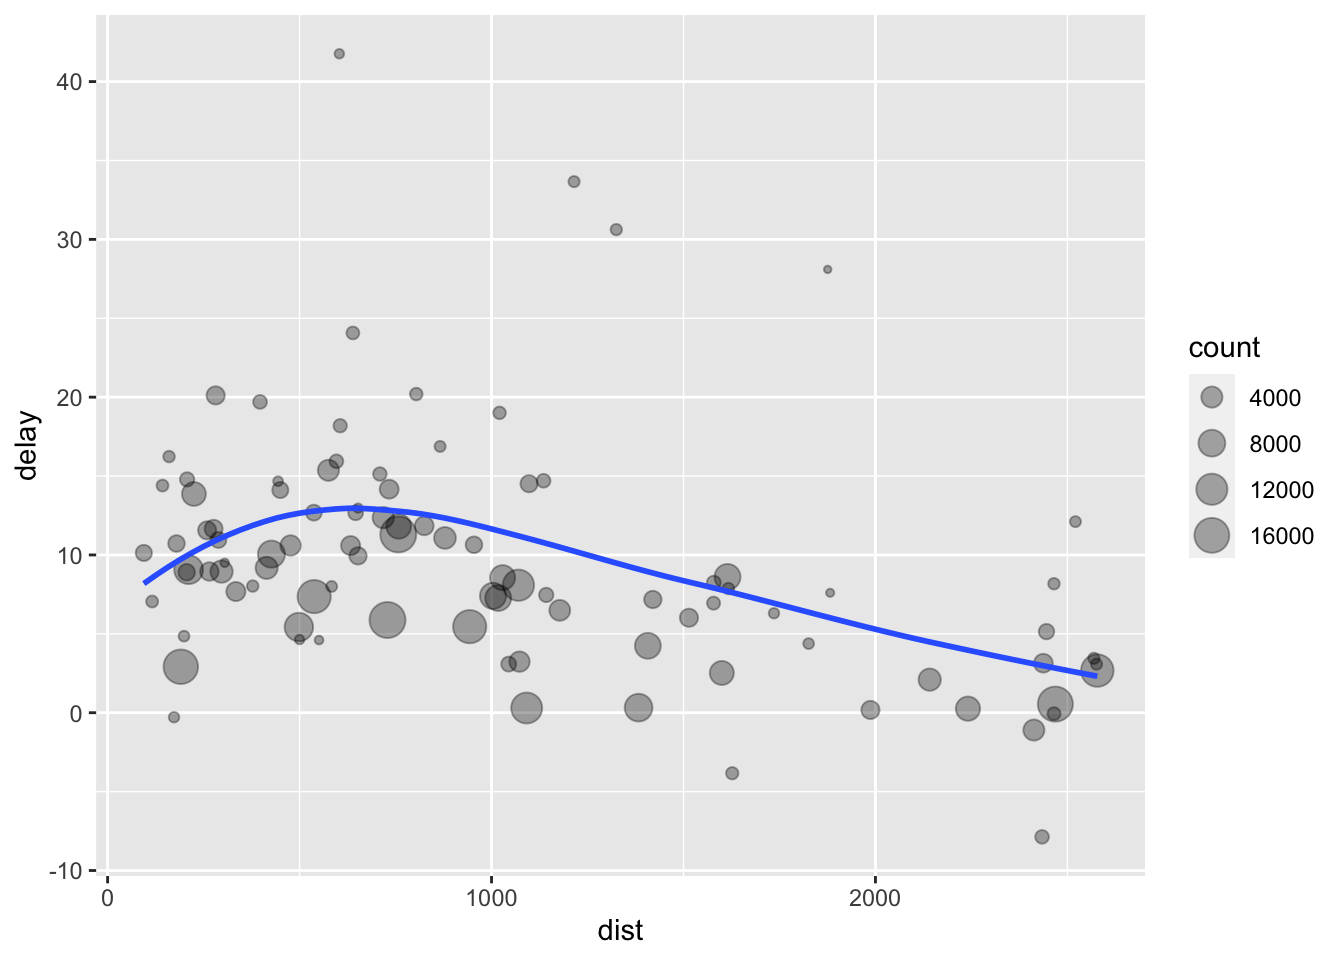
\includegraphics{Dinamica_poblacional_files/figure-latex/unnamed-chunk-66-1.pdf}

\begin{Shaded}
\begin{Highlighting}[]
\FunctionTok{library}\NormalTok{(Rcompadre)}
\FunctionTok{library}\NormalTok{(popdemo)}
\FunctionTok{data}\NormalTok{(Compadre)}


\NormalTok{Compadre}\SpecialCharTok{$}\NormalTok{matA }\OtherTok{\textless{}{-}} \FunctionTok{matA}\NormalTok{(Compadre)}

\CommentTok{\# create empty vector to store output}
\NormalTok{Compadre}\SpecialCharTok{$}\NormalTok{dim }\OtherTok{\textless{}{-}} \FunctionTok{numeric}\NormalTok{(}\FunctionTok{nrow}\NormalTok{(Compadre))}

\NormalTok{index}\SpecialCharTok{$}\NormalTok{dim }\OtherTok{\textless{}{-}} \FunctionTok{numeric}\NormalTok{(}\FunctionTok{nrow}\NormalTok{(index\_O))}
\end{Highlighting}
\end{Shaded}

\begin{verbatim}
## Warning in index$dim <- numeric(nrow(index_O)): Coercing LHS to a list
\end{verbatim}

\begin{Shaded}
\begin{Highlighting}[]
\CommentTok{\# loop through all rows of Compadre}
\ControlFlowTok{for}\NormalTok{ (i }\ControlFlowTok{in} \FunctionTok{seq\_len}\NormalTok{(}\FunctionTok{nrow}\NormalTok{(Compadre))) \{}
\NormalTok{  Compadre}\SpecialCharTok{$}\NormalTok{dim[i] }\OtherTok{\textless{}{-}} \FunctionTok{nrow}\NormalTok{(Compadre}\SpecialCharTok{$}\NormalTok{matA[[i]])}
\NormalTok{\}}

\CommentTok{\# function to determine whether matrix \textquotesingle{}mat\textquotesingle{} has any stages with no transitions}
\NormalTok{NullStages }\OtherTok{\textless{}{-}} \ControlFlowTok{function}\NormalTok{(mat) }\FunctionTok{any}\NormalTok{(}\FunctionTok{colSums}\NormalTok{(mat) }\SpecialCharTok{==} \DecValTok{0}\NormalTok{)}

\CommentTok{\# apply function to every element of A}
\NormalTok{Compadre}\SpecialCharTok{$}\NormalTok{null\_stages }\OtherTok{\textless{}{-}} \FunctionTok{sapply}\NormalTok{(Compadre}\SpecialCharTok{$}\NormalTok{matA, NullStages)}

\FunctionTok{NullStages}\NormalTok{(Compadre}\SpecialCharTok{$}\NormalTok{matA[[}\DecValTok{1}\NormalTok{]]) }\CommentTok{\# apply function to single element}
\end{Highlighting}
\end{Shaded}

\begin{verbatim}
## [1] FALSE
\end{verbatim}

\begin{Shaded}
\begin{Highlighting}[]
\NormalTok{Compadre}\SpecialCharTok{$}\NormalTok{null\_stages }\OtherTok{\textless{}{-}} \FunctionTok{sapply}\NormalTok{(}\FunctionTok{matA}\NormalTok{(Compadre), NullStages)}
\end{Highlighting}
\end{Shaded}

\hypertarget{traduccion-del-articulo-protocolo-de-informaciuxf3n}{%
\chapter{Traduccion del articulo Protocolo de información}\label{traduccion-del-articulo-protocolo-de-informaciuxf3n}}

Por: Grupo de Anne

\hypertarget{dinuxe1mica-espacial-y-temporal-de-encyclia-bocourtii-despuuxe9s-de-15-auxf1os-en-la-penuxednsula-de-guanahacabibes-cuba}{%
\chapter{Dinámica espacial y temporal de Encyclia bocourtii después de 15 años en la Península de Guanahacabibes, Cuba}\label{dinuxe1mica-espacial-y-temporal-de-encyclia-bocourtii-despuuxe9s-de-15-auxf1os-en-la-penuxednsula-de-guanahacabibes-cuba}}

Por: Ernesto y Elaine

\hypertarget{nhora}{%
\chapter{Nhora}\label{nhora}}

Por: Nhora

\hypertarget{impactos-de-datos-sin-sentido-sobre-los-analisis}{%
\chapter{Impactos de datos sin sentido sobre los analisis}\label{impactos-de-datos-sin-sentido-sobre-los-analisis}}

Por: RLT

\hypertarget{hojas-de-datos-en-el-campo}{%
\chapter{Hojas de datos en el campo}\label{hojas-de-datos-en-el-campo}}

Por: RLT, Nhora, Demetria, Anne\ldots.

La hoja de recoleccion de datos deberia estar preparada antes de ir al campo y estar sobre papel que es impermeable y escribir con lapiz. Ese ultimo punto es bien importante ya que la gran mayoria de los boligrafos son soluble en agua y si el papel se moja ud puede perder sus daos. RECUERDA que no se puede regresar en el tiempo y recoger los datos. Si Ud tiene su hoja de datos en el laboratorio y se le cae la taza cafe y fue escrito con boligrafo se puede perder los datos. No se arriega.

es importante tener la lista completa de todos los individuos en la hoja de datos, ya que esto le ayuda asegurarse durante el muestreo que no se le olvida ningun individuo. Datos olvidado no se puede recuperar

Hoja en blanco para llevarse

\begin{Shaded}
\begin{Highlighting}[]
\FunctionTok{library}\NormalTok{(tidyverse)}
\FunctionTok{library}\NormalTok{(gt)}
\NormalTok{Hoja\_de\_campo }\OtherTok{=} \FunctionTok{tribble}\NormalTok{(}
  \SpecialCharTok{\textasciitilde{}}\NormalTok{Número\_de\_Ind, }\SpecialCharTok{\textasciitilde{}}\NormalTok{Etapa, }\SpecialCharTok{\textasciitilde{}}\NormalTok{Cantidad\_flores\_abierta, }\SpecialCharTok{\textasciitilde{}}\NormalTok{Cantidad\_capullo, }\SpecialCharTok{\textasciitilde{}}\NormalTok{ Cantidad\_Frutos, }\SpecialCharTok{\textasciitilde{}}\NormalTok{Numero\_Hojas, }\SpecialCharTok{\textasciitilde{}}\NormalTok{Ancho\_hoja\_mm, }\SpecialCharTok{\textasciitilde{}}\NormalTok{etc,}
  \DecValTok{23001}\NormalTok{,}\StringTok{"..."}\NormalTok{,}\StringTok{"..."}\NormalTok{,}\StringTok{"..."}\NormalTok{,}\StringTok{"..."}\NormalTok{,}\StringTok{"..."}\NormalTok{,}\StringTok{"..."}\NormalTok{,}\StringTok{"..."}\NormalTok{,}
  \DecValTok{23002}\NormalTok{,}\StringTok{"..."}\NormalTok{,}\StringTok{"..."}\NormalTok{,}\StringTok{"..."}\NormalTok{,}\StringTok{"..."}\NormalTok{,}\StringTok{"..."}\NormalTok{,}\StringTok{"..."}\NormalTok{,}\StringTok{"..."}\NormalTok{,}
  \DecValTok{23003}\NormalTok{,}\StringTok{"..."}\NormalTok{,}\StringTok{"..."}\NormalTok{,}\StringTok{"..."}\NormalTok{,}\StringTok{"..."}\NormalTok{,}\StringTok{"..."}\NormalTok{,}\StringTok{"..."}\NormalTok{,}\StringTok{"..."}\NormalTok{,}
  \DecValTok{23004}\NormalTok{,}\StringTok{"..."}\NormalTok{,}\StringTok{"..."}\NormalTok{,}\StringTok{"..."}\NormalTok{,}\StringTok{"..."}\NormalTok{,}\StringTok{"..."}\NormalTok{,}\StringTok{"..."}\NormalTok{,}\StringTok{"..."}\NormalTok{,}
  \DecValTok{23005}\NormalTok{,}\StringTok{"..."}\NormalTok{,}\StringTok{"..."}\NormalTok{,}\StringTok{"..."}\NormalTok{,}\StringTok{"..."}\NormalTok{,}\StringTok{"..."}\NormalTok{,}\StringTok{"..."}\NormalTok{,}\StringTok{"..."}\NormalTok{,}
  \DecValTok{24006}\NormalTok{,}\StringTok{"..."}\NormalTok{,}\StringTok{"..."}\NormalTok{,}\StringTok{"..."}\NormalTok{,}\StringTok{"..."}\NormalTok{,}\StringTok{"..."}\NormalTok{,}\StringTok{"..."}\NormalTok{,}\StringTok{"..."}\NormalTok{,}
  \DecValTok{24007}\NormalTok{,}\StringTok{"..."}\NormalTok{,}\StringTok{"..."}\NormalTok{,}\StringTok{"..."}\NormalTok{,}\StringTok{"..."}\NormalTok{,}\StringTok{"..."}\NormalTok{,}\StringTok{"..."}\NormalTok{,}\StringTok{"..."}\NormalTok{,}
  \DecValTok{24008}\NormalTok{,}\StringTok{"..."}\NormalTok{,}\StringTok{"..."}\NormalTok{,}\StringTok{"..."}\NormalTok{,}\StringTok{"..."}\NormalTok{,}\StringTok{"..."}\NormalTok{,}\StringTok{"..."}\NormalTok{,}\StringTok{"..."}\NormalTok{,}
  
\NormalTok{)}

\NormalTok{Hoja\_de\_campo }\SpecialCharTok{\%\textgreater{}\%} \FunctionTok{gt}\NormalTok{()}
\end{Highlighting}
\end{Shaded}

\begin{longtable}{rrrrrrrr}
\toprule
Número\_de\_Ind & Etapa & Cantidad\_flores\_abierta & Cantidad\_capullo & Cantidad\_Frutos & Numero\_Hojas & Ancho\_hoja\_mm & etc \\ 
\midrule
23001 & ... & ... & ... & ... & ... & ... & ... \\ 
23002 & ... & ... & ... & ... & ... & ... & ... \\ 
23003 & ... & ... & ... & ... & ... & ... & ... \\ 
23004 & ... & ... & ... & ... & ... & ... & ... \\ 
23005 & ... & ... & ... & ... & ... & ... & ... \\ 
24006 & ... & ... & ... & ... & ... & ... & ... \\ 
24007 & ... & ... & ... & ... & ... & ... & ... \\ 
24008 & ... & ... & ... & ... & ... & ... & ... \\ 
\bottomrule
\end{longtable}

Usando ejemplo de Tremblay {[}{]} y su codificación

\begin{itemize}
\tightlist
\item
  p == \textbf{plantula}.
\item
  j == \textbf{juvenil}
\item
  A0 == \textbf{adulto non-reproductivo}
\item
  A1 == \textbf{adulto reproductivo}
\item
  M = \textbf{muerto}
\end{itemize}

Hoja llena al final del muestreo

\begin{Shaded}
\begin{Highlighting}[]
\FunctionTok{library}\NormalTok{(tidyverse)}
\FunctionTok{library}\NormalTok{(gt)}
\NormalTok{Hoja\_llena }\OtherTok{=} \FunctionTok{tribble}\NormalTok{(}
  \SpecialCharTok{\textasciitilde{}}\NormalTok{Número\_de\_Ind, }\SpecialCharTok{\textasciitilde{}}\NormalTok{Etapa, }\SpecialCharTok{\textasciitilde{}}\NormalTok{Cantidad\_flores\_abierta, }\SpecialCharTok{\textasciitilde{}}\NormalTok{Cantidad\_capullo, }\SpecialCharTok{\textasciitilde{}}\NormalTok{ Cantidad\_Frutos, }\SpecialCharTok{\textasciitilde{}}\NormalTok{Numero\_Hojas, }\SpecialCharTok{\textasciitilde{}}\NormalTok{Ancho\_hoja\_mm, }\SpecialCharTok{\textasciitilde{}}\NormalTok{etc,}
  \DecValTok{23001}\NormalTok{,}\StringTok{"p"}\NormalTok{,}\ConstantTok{NA}\NormalTok{, }\ConstantTok{NA}\NormalTok{,}\ConstantTok{NA}\NormalTok{,}\ConstantTok{NA}\NormalTok{,}\ConstantTok{NA}\NormalTok{,}\ConstantTok{NA}\NormalTok{,}
  \DecValTok{23002}\NormalTok{,}\StringTok{"j"}\NormalTok{,}\ConstantTok{NA}\NormalTok{, }\ConstantTok{NA}\NormalTok{,}\ConstantTok{NA}\NormalTok{,}\DecValTok{2}\NormalTok{,}\DecValTok{10}\NormalTok{,}\ConstantTok{NA}\NormalTok{,}
  \DecValTok{23003}\NormalTok{,}\StringTok{"A1"}\NormalTok{,}\DecValTok{5}\NormalTok{, }\DecValTok{10}\NormalTok{,}\DecValTok{1}\NormalTok{, }\DecValTok{5}\NormalTok{,}\DecValTok{32}\NormalTok{,}\ConstantTok{NA}\NormalTok{,}
  \DecValTok{23004}\NormalTok{,}\StringTok{"Ao"}\NormalTok{,}\DecValTok{0}\NormalTok{, }\DecValTok{0}\NormalTok{,}\DecValTok{0}\NormalTok{,}\DecValTok{2}\NormalTok{,}\DecValTok{14}\NormalTok{,}\ConstantTok{NA}\NormalTok{,}
  \DecValTok{23005}\NormalTok{,}\StringTok{"m"}\NormalTok{,}\ConstantTok{NA}\NormalTok{, }\ConstantTok{NA}\NormalTok{,}\ConstantTok{NA}\NormalTok{,}\ConstantTok{NA}\NormalTok{,}\ConstantTok{NA}\NormalTok{,}\ConstantTok{NA}\NormalTok{,}
  \DecValTok{24006}\NormalTok{,}\StringTok{"p"}\NormalTok{,}\ConstantTok{NA}\NormalTok{, }\ConstantTok{NA}\NormalTok{,}\ConstantTok{NA}\NormalTok{,}\ConstantTok{NA}\NormalTok{,}\ConstantTok{NA}\NormalTok{,}\ConstantTok{NA}\NormalTok{,}
  \DecValTok{24007}\NormalTok{,}\StringTok{"j"}\NormalTok{,}\ConstantTok{NA}\NormalTok{, }\ConstantTok{NA}\NormalTok{,}\ConstantTok{NA}\NormalTok{,}\DecValTok{1}\NormalTok{,}\DecValTok{7}\NormalTok{,}\ConstantTok{NA}\NormalTok{,}
  \DecValTok{24008}\NormalTok{,}\StringTok{"p"}\NormalTok{,}\ConstantTok{NA}\NormalTok{, }\ConstantTok{NA}\NormalTok{,}\ConstantTok{NA}\NormalTok{,}\ConstantTok{NA}\NormalTok{,}\ConstantTok{NA}\NormalTok{,}\ConstantTok{NA}\NormalTok{,}
  
\NormalTok{)}

\NormalTok{Hoja\_llena }\SpecialCharTok{\%\textgreater{}\%} \FunctionTok{gt}\NormalTok{()}
\end{Highlighting}
\end{Shaded}

\begin{longtable}{rlrrrrrc}
\toprule
Número\_de\_Ind & Etapa & Cantidad\_flores\_abierta & Cantidad\_capullo & Cantidad\_Frutos & Numero\_Hojas & Ancho\_hoja\_mm & etc \\ 
\midrule
23001 & p & NA & NA & NA & NA & NA & NA \\ 
23002 & j & NA & NA & NA & 2 & 10 & NA \\ 
23003 & A1 & 5 & 10 & 1 & 5 & 32 & NA \\ 
23004 & Ao & 0 & 0 & 0 & 2 & 14 & NA \\ 
23005 & m & NA & NA & NA & NA & NA & NA \\ 
24006 & p & NA & NA & NA & NA & NA & NA \\ 
24007 & j & NA & NA & NA & 1 & 7 & NA \\ 
24008 & p & NA & NA & NA & NA & NA & NA \\ 
\bottomrule
\end{longtable}

Nota que solamente los individuos 23003 y 23004 son adultos, uno tiene flores, capullos y frutos y el otro nada. A todos los adultos hay que llenar la informacion, no dejarlo en blanco. Para las otras etapas, no es necesario llenar la mayoria de las columnas ya que para las plantulas y muertos no PUEDEN tener esas, pero los juveniles, se puede llenar la cantidad de hojas y sus tamaño. Nota que el individuo 23005 se murio.

Esa misma estructura de recoger los dados puede ser utilizado para ponerlo en una hoja de MSExcel, Google Sheet o MacOS Numbers.

\hypertarget{intro}{%
\chapter{Nombre del capitulo.}\label{intro}}

All chapters start with a first-level heading followed by your chapter title, like the line above. There should be only one first-level heading (\texttt{\#}) per .Rmd file.

\hypertarget{a-section}{%
\section{A section}\label{a-section}}

\hypertarget{otra-seccion}{%
\section{Otra seccion}\label{otra-seccion}}

All chapter sections start with a second-level (\texttt{\#\#}) or higher heading followed by your section title, like the sections above and below here. You can have as many as you want within a chapter.

\hypertarget{a-subsection}{%
\subsection*{A subsection}\label{a-subsection}}
\addcontentsline{toc}{subsection}{A subsection}

The subtopic

\hypertarget{section-2}{%
\subsubsection{}\label{section-2}}

More subdivision

\hypertarget{section-3}{%
\paragraph{}\label{section-3}}

Even more subdivision

\hypertarget{an-unnumbered-section}{%
\subsection*{An unnumbered section}\label{an-unnumbered-section}}
\addcontentsline{toc}{subsection}{An unnumbered section}

Chapters and sections are numbered by default. To un-number a heading, add a \texttt{\{.unnumbered\}} or the shorter \texttt{\{-\}} at the end of the heading, like in this section.

Remember not to use only 1 \emph{\#} as this indicates a new chapter

\hypertarget{note-the-size-of-font-changes-with-the-number}{%
\section{\texorpdfstring{NOTE the size of font changes with the number \emph{\#}}{NOTE the size of font changes with the number \#}}\label{note-the-size-of-font-changes-with-the-number}}

\hypertarget{note-the-size-of-font-changes-with-the-number-1}{%
\subsection{\texorpdfstring{NOTE the size of font changes with the number \emph{\#}}{NOTE the size of font changes with the number \#}}\label{note-the-size-of-font-changes-with-the-number-1}}

\hypertarget{note-the-size-of-font-changes-with-the-number-2}{%
\subsubsection{\texorpdfstring{NOTE the size of font changes with the number \emph{\#}}{NOTE the size of font changes with the number \#}}\label{note-the-size-of-font-changes-with-the-number-2}}

\hypertarget{note-the-size-of-font-changes-with-the-number-3}{%
\paragraph{\texorpdfstring{NOTE the size of font changes with the number \emph{\#}}{NOTE the size of font changes with the number \#}}\label{note-the-size-of-font-changes-with-the-number-3}}

Don't miss Table \ref{tab:nice-table}.

\hypertarget{cross}{%
\chapter{Cross-references}\label{cross}}

Cross-references make it easier for your readers to find and link to elements in your book.

\hypertarget{chapters-and-sub-chapters}{%
\section{Chapters and sub-chapters}\label{chapters-and-sub-chapters}}

There are two steps to cross-reference any heading:

\begin{enumerate}
\def\labelenumi{\arabic{enumi}.}
\item
  Label the heading: \texttt{\#\ Hello\ world\ \{\#nice-label\}}.

  \begin{itemize}
  \item
    Leave the label off if you like the automated heading generated based on your heading title: for example, \texttt{\#\ Hello\ world} = \texttt{\#\ Hello\ world\ \{\#hello-world\}}.
  \item
    To label an un-numbered heading, use: \texttt{\#\ Hello\ world\ \{-\#nice-label\}} or \texttt{\{\#\ Hello\ world\ .unnumbered\}}.
  \end{itemize}
\item
  Next, reference the labeled heading anywhere in the text using \texttt{\textbackslash{}@ref(nice-label)}; for example, please see Chapter \ref{intro}.

  \begin{itemize}
  \tightlist
  \item
    If you prefer text as the link instead of a numbered reference use: \protect\hyperlink{cross}{any text you want can go here}.
  \end{itemize}
\end{enumerate}

\begin{center}\rule{0.5\linewidth}{0.5pt}\end{center}

\hypertarget{captioned-figures-and-tables}{%
\section{Captioned figures and tables}\label{captioned-figures-and-tables}}

Figures and tables \emph{with captions} can also be cross-referenced from elsewhere in your book using \texttt{\textbackslash{}@ref(fig:chunk-label)} and \texttt{\textbackslash{}@ref(tab:chunk-label)}, respectively.

See Figure \ref{fig:nice-fig}.

\begin{Shaded}
\begin{Highlighting}[]
\FunctionTok{par}\NormalTok{(}\AttributeTok{mar =} \FunctionTok{c}\NormalTok{(}\DecValTok{4}\NormalTok{, }\DecValTok{4}\NormalTok{, .}\DecValTok{1}\NormalTok{, .}\DecValTok{1}\NormalTok{))}
\FunctionTok{plot}\NormalTok{(pressure, }\AttributeTok{type =} \StringTok{\textquotesingle{}b\textquotesingle{}}\NormalTok{, }\AttributeTok{pch =} \DecValTok{19}\NormalTok{)}
\end{Highlighting}
\end{Shaded}

\begin{figure}

{\centering 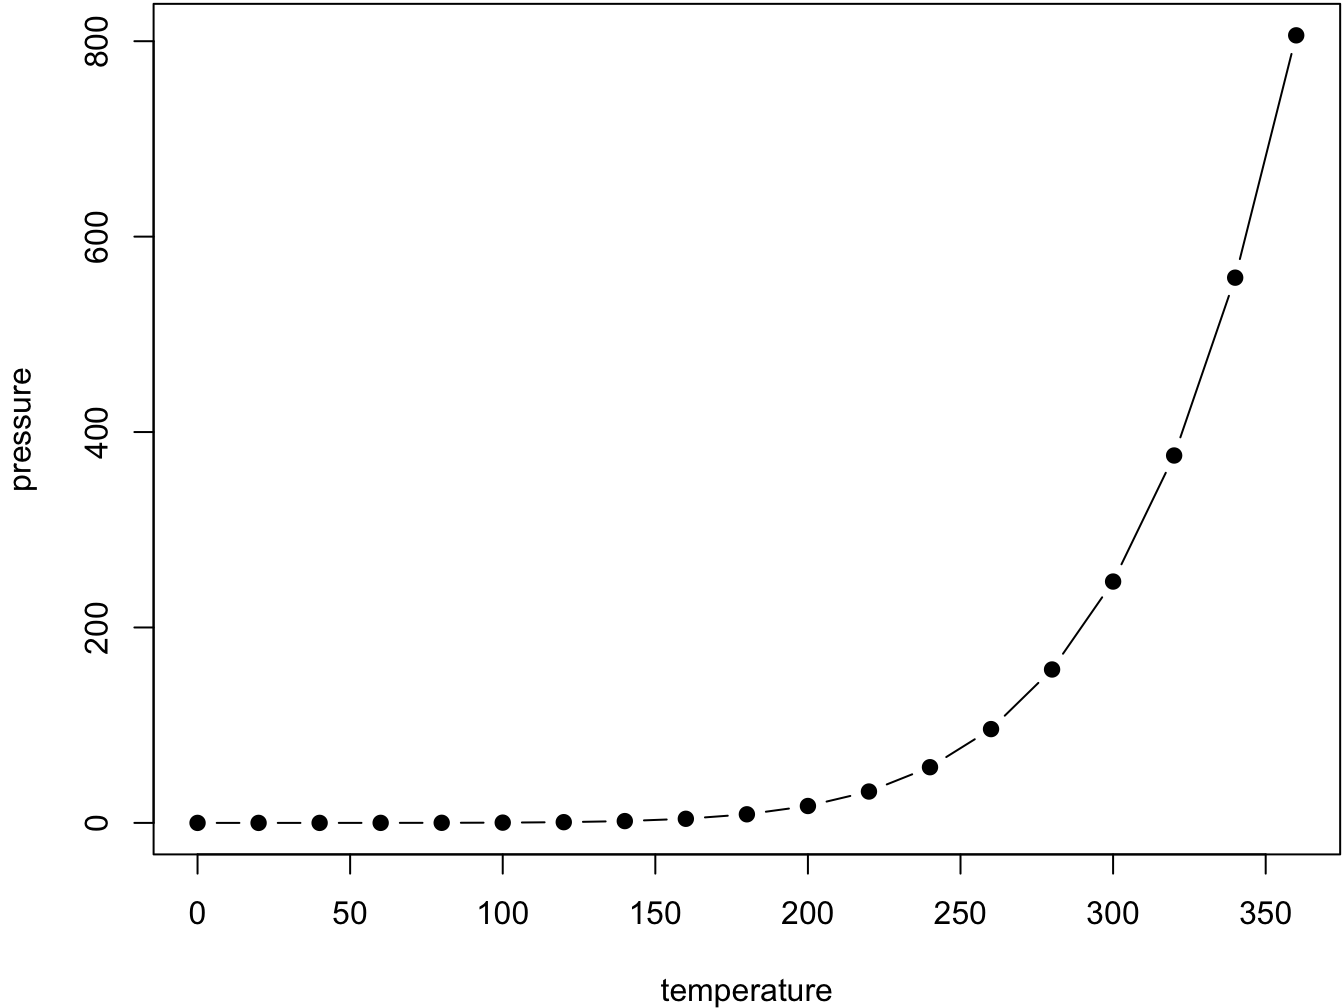
\includegraphics[width=0.8\linewidth]{Dinamica_poblacional_files/figure-latex/nice-fig-1} 

}

\caption{Here is a nice figure!}\label{fig:nice-fig}
\end{figure}

Don't miss Table \ref{tab:nice-table}.

\begin{Shaded}
\begin{Highlighting}[]
\NormalTok{knitr}\SpecialCharTok{::}\FunctionTok{kable}\NormalTok{(}
  \FunctionTok{head}\NormalTok{(pressure, }\DecValTok{10}\NormalTok{), }\AttributeTok{caption =} \StringTok{\textquotesingle{}Here is a nice table!\textquotesingle{}}\NormalTok{,}
  \AttributeTok{booktabs =} \ConstantTok{TRUE}
\NormalTok{)}
\end{Highlighting}
\end{Shaded}

\begin{table}

\caption{\label{tab:nice-table}Here is a nice table!}
\centering
\begin{tabular}[t]{rr}
\toprule
temperature & pressure\\
\midrule
0 & 0.0002\\
20 & 0.0012\\
40 & 0.0060\\
60 & 0.0300\\
80 & 0.0900\\
\addlinespace
100 & 0.2700\\
120 & 0.7500\\
140 & 1.8500\\
160 & 4.2000\\
180 & 8.8000\\
\bottomrule
\end{tabular}
\end{table}

\hypertarget{appendix-list-of-epiphyitc-species}{%
\chapter*{(Appendix) List of epiphyitc species}\label{appendix-list-of-epiphyitc-species}}
\addcontentsline{toc}{chapter}{(Appendix) List of epiphyitc species}

You can add parts to organize one or more book chapters together. Parts can be inserted at the top of an .Rmd file, before the first-level chapter heading in that same file.

Add a numbered part: \texttt{\#\ (PART)\ Act\ one\ \{-\}} (followed by \texttt{\#\ A\ chapter})

Add an unnumbered part: \texttt{\#\ (PART\textbackslash{}*)\ Act\ two\ \{-\}} (followed by \texttt{\#\ A\ chapter})

Add an appendix as a special kind of un-numbered part: \texttt{\#\ (APPENDIX)\ Other\ stuff\ \{-\}} (followed by \texttt{\#\ A\ chapter}). Chapters in an appendix are prepended with letters instead of numbers.

\hypertarget{appendix-list-of-terrestrial-species}{%
\chapter*{(Appendix) List of terrestrial species}\label{appendix-list-of-terrestrial-species}}
\addcontentsline{toc}{chapter}{(Appendix) List of terrestrial species}

\hypertarget{footnotes-and-citations}{%
\chapter{Footnotes and citations}\label{footnotes-and-citations}}

\hypertarget{footnotes}{%
\section{Footnotes}\label{footnotes}}

Footnotes are put inside the square brackets after a caret \texttt{\^{}{[}{]}}. Like this one \footnote{This is a footnote.}.

Let's add a second footnote. In this case we add information on the origin of matrix algebra \footnote{The term matrix was introduced by the 19th-century English mathematician James Sylvester, but it was his friend the mathematician Arthur Cayley who developed the algebraic aspect of matrices in two papers in the 1850s.}

Mi tercer footnote es filosofico \footnote{kgjljgljhggjlhgjhgljgjhl}

\hypertarget{citations}{%
\section{Citations}\label{citations}}

Reference items in your bibliography file(s) using \texttt{@key}.

For example, we are using the \textbf{bookdown} package \citep{R-bookdown} (check out the last code chunk in index.Rmd to see how this citation key was added) in this sample book, which was built on top of R Markdown and \textbf{knitr} \citep{xie2015} (this citation was added manually in an external file book.bib).
Note that the \texttt{.bib} files need to be listed in the index.Rmd with the YAML \texttt{bibliography} key.

\hypertarget{here-is-second-citation.}{%
\subsubsection{Here is second citation.}\label{here-is-second-citation.}}

Evolutionary processes in orchids are likely to be a interaction between natural selection and genetic drift \citep{tremblay2005variation}.

\hypertarget{here-is-a-third-citation}{%
\subsubsection{Here is a third citation}\label{here-is-a-third-citation}}

un articulo de Damon excepcional \citep{damon2000review}

\hypertarget{links-to-websites}{%
\section{Links to websites}\label{links-to-websites}}

The RStudio Visual Markdown Editor can also make it easier to insert citations: \url{https://rstudio.github.io/visual-markdown-editing/\#/citations}

\url{https://www.researchgate.net/profile/Raymond-Tremblay}

\hypertarget{blocks}{%
\chapter{Blocks}\label{blocks}}

\hypertarget{equations}{%
\section{Equations}\label{equations}}

Here is an equation.

\begin{equation} 
  f\left(k\right) = \binom{n}{k} p^k\left(1-p\right)^{n-k}
  \label{eq:binom} 
\end{equation}

You may refer to using \texttt{\textbackslash{}@ref(eq:binom)}, like see Equation \eqref{eq:binom}.

-- this is the script to make the equation connectable in the text

** that the \texttt{....} are to make the text visual

\hypertarget{theorems-and-proofs}{%
\section{Theorems and proofs}\label{theorems-and-proofs}}

Labeled theorems can be referenced in text using \texttt{\textbackslash{}@ref(thm:tri)}, for example, check out this smart theorem \ref{thm:tri}.

::: \{.theorem \#tri\}
For a right triangle, if \(c\) denotes the \emph{length} of the hypotenuse
and \(a\) and \(b\) denote the lengths of the \textbf{other} two sides, we have
\[a^2 + b^2 = c^2\]

A site to help create your equations \[\bar{x}=\frac{\sum x_{i}}{n}\]

\url{https://latex.codecogs.com/eqneditor/editor.php}

Ahora se enseña la formula del promedio \ref{thm:promedio}

\begin{theorem}
\protect\hypertarget{thm:promedio}{}\label{thm:promedio}\[\bar{x}= \frac{\sum x_{i}}{n}\]

Si quiere la ecuación en la linea usa solamente un ``\$'' antes y despues de la formula.
El promedio tiene la siguiente formula \(\bar{x}= \frac{\sum x_{i}}{n}\) y la varianza se estima tomando la diferencia entre los valores y el promedio.
\end{theorem}

Read more here \url{https://bookdown.org/yihui/bookdown/markdown-extensions-by-bookdown.html}.

\begin{center}\rule{0.5\linewidth}{0.5pt}\end{center}

\hypertarget{callout-blocks}{%
\section{Callout blocks}\label{callout-blocks}}

The R Markdown Cookbook provides more help on how to use custom blocks to design your own callouts: \url{https://bookdown.org/yihui/rmarkdown-cookbook/custom-blocks.html}

\hypertarget{sharing-your-book}{%
\chapter{Sharing your book}\label{sharing-your-book}}

\hypertarget{publishing}{%
\section{Publishing}\label{publishing}}

HTML books can be published online, see: \url{https://bookdown.org/yihui/bookdown/publishing.html}

\hypertarget{pages}{%
\section{404 pages}\label{pages}}

By default, users will be directed to a 404 page if they try to access a webpage that cannot be found. If you'd like to customize your 404 page instead of using the default, you may add either a \texttt{\_404.Rmd} or \texttt{\_404.md} file to your project root and use code and/or Markdown syntax.

\hypertarget{metadata-for-sharing}{%
\section{Metadata for sharing}\label{metadata-for-sharing}}

Bookdown HTML books will provide HTML metadata for social sharing on platforms like Twitter, Facebook, and LinkedIn, using information you provide in the \texttt{index.Rmd} YAML. To setup, set the \texttt{url} for your book and the path to your \texttt{cover-image} file. Your book's \texttt{title} and \texttt{description} are also used.

This \texttt{gitbook} uses the same social sharing data across all chapters in your book- all links shared will look the same.

Specify your book's source repository on GitHub using the \texttt{edit} key under the configuration options in the \texttt{\_output.yml} file, which allows users to suggest an edit by linking to a chapter's source file.

Read more about the features of this output format here:

\url{https://pkgs.rstudio.com/bookdown/reference/gitbook.html}

Or use:

\begin{Shaded}
\begin{Highlighting}[]
\NormalTok{?bookdown}\SpecialCharTok{::}\NormalTok{gitbook}
\end{Highlighting}
\end{Shaded}


  \bibliography{book.bib,packages.bib}

\end{document}
